% Punto decimal también en modo matemático (babel-spanish lo vuelve coma); vale desde aquí hasta el final.
\ifdefined\decimalpoint\decimalpoint\else\mathcode`\.="013A \fi


\chapter{Mezclas DDP para Series de Tiempo Funcionales}
\label{03_00_00_mezclas_ddp_series_tiempo_funcionales}

Este capítulo presenta el PSBPM-FD, el modelo propuesto en esta tesis, que estima la distribución condicional completa de la curva siguiente dado el pasado del proceso, de modo que no solo su nivel sino también su dispersión y su número de modos puedan cambiar con el estado reciente. Esa es la propiedad que un modelo de media lineal con ley de innovación fija no tiene, y el capítulo parte de ahí, la Sección~\ref{03_01_00_motivacion} muestra por qué los modelos funcionales lineales y los métodos de aprendizaje automático no la ofrecen, y la Sección~\ref{03_02_00_estado_arte} revisa la literatura bayesiana no paramétrica para series de tiempo y datos funcionales y delimita la brecha que el trabajo busca cubrir.\\

El modelo se construye en las Secciones~\ref{03_03_00_psbp} y~\ref{03_04_00_modelo_propuesto_psbpm_fd}. La primera presenta el Probit Stick-Breaking Process Mixture de \citet{03_02_chung2009nonparametric} con su esquema de inferencia, y la segunda lo lleva al caso en que las observaciones son curvas y los predictores son el pasado del propio proceso. Las curvas se representan mediante sus componentes principales funcionales y la dinámica de cada score se modela con una mezcla probit stick-breaking de regresiones normales cuyos pesos dependen de los scores rezagados, de manera que la forma de la ley cambia cuando cambia el estado del proceso. La Sección~\ref{03_05_00_reconstruccion_funcional} transporta la predictiva de los scores a la curva y define sobre ella los resúmenes con que se pronostica, los predictores puntuales y los intervalos de credibilidad, y la Sección~\ref{03_06_00_comportamientos} presenta los comportamientos predictivos, que distinguen en cada origen los desenlaces posibles de la curva siguiente y la probabilidad de cada uno.\\

El desempeño del modelo se analiza en las Secciones~\ref{03_07_00_diseno_estudio_simulacion} y~\ref{03_08_00_resultados} mediante un estudio de simulación, en el que se conoce el proceso que genera los datos y es posible contrastar lo estimado con lo verdadero. Los tres escenarios se construyen para que la ley condicional tenga un rasgo que un modelo de media lineal no representa, heterocedasticidad condicional, cambio de régimen por umbral o multimodalidad en la ley de los scores, y sobre ellos se evalúan, frente al FAR y a un Random Forest, la predicción puntual, los intervalos de credibilidad y, en el escenario con cambio de régimen, los comportamientos y el pronóstico que se construye con ellos. 

\section{Motivación}
\label{03_01_00_motivacion}
 
Al igual que en el contexto escalar y multivariado, donde la dependencia temporal se captura mediante la distribución condicional de $X_t$ dado su historia $\{X_{t-1}, X_{t-2}, \ldots\}$, en las series de tiempo funcionales el objetivo es análogo, es decir, caracterizar la ley condicional de la curva $X_t(\tau)$ dado el conjunto de curvas pasadas $\{X_{t-1}(\tau), X_{t-2}(\tau), \ldots\}$. Así como en el caso clásico existen múltiples metodologías para modelar dicha dependencia, en el contexto funcional el abanico de estrategias se amplía aún más, precisamente porque cada observación ya no es un escalar o un vector de dimensión finita sino una curva que vive en un espacio funcional de dimensión infinita.\\
 
La estrategia más común consiste en extender los modelos clásicos de series de tiempo al contexto funcional, es decir, utilizar los modelos funcionales FAR, FMA y FARMA, los cuales postulan una dinámica lineal gobernada por un operador acotado sobre el espacio de funciones, \citep{02_02_bosq2000linear}. Otra estrategia recurre a esquemas de reducción de dimensión, en los cuales se proyectan las curvas sobre una base de componentes principales funcionales y se modelan por separado las series de scores resultantes mediante técnicas clásicas univariadas, \citep{03_00_hyndman2007robust,03_00_hyndman2009forecasting}, o bien mediante un modelo vectorial autorregresivo sobre el vector de scores, \citep{02_02_aue2015prediction}. Ambos enfoques incorporan explícitamente la dependencia temporal entre observaciones funcionales y permiten cuantificar la incertidumbre predictiva; sin embargo, heredan limitaciones estructurales. En primer lugar, la dinámica se restringe a un operador lineal actuando sobre la curva (o el vector de scores) rezagado, de modo que la distribución condicional de $X_t$ dado su pasado queda completamente determinada por una única ley de innovación homogénea en el tiempo, es decir, el modelo podría no admitir multimodalidad condicional, asimetrías dependientes del estado, una dispersión que cambie con la historia reciente ni regímenes dinámicos cambiantes. En segundo lugar, la teoría de estimación y predicción descansa en supuestos de estacionariedad, \citep{03_00_hormann2010weakly,02_02_aue2015prediction} cuya violación ha sido documentada empíricamente en aplicaciones prácticas como las curvas de precios intradiarios, \citet{03_00_horvath2014testing}, y las curvas de temperatura, \citet{03_00_aue2018detecting}, donde la hipótesis de estacionariedad resulta rechazada y motiva por tanto el estudio de otras metodologías.\\
 
Paralelamente, los avances en aprendizaje automático han dado lugar a modelos altamente flexibles, como redes neuronales, Random Forest y máquinas de soporte vectorial, con aplicaciones directas al pronóstico de series de tiempo funcionales, típicamente operando sobre los scores de una descomposición en componentes principales funcionales, \citep{03_00_forecast4010022}. Estos métodos relajan la restricción de linealidad en la media condicional y exhiben, en general, un elevado poder predictivo puntual. No obstante, sus limitaciones para el problema que aquí interesa son de naturaleza distribucional. En primer lugar, estos métodos producen pronósticos puntuales sin medida de incertidumbre asociada, de modo que su cuantificación debe añadirse externamente al modelo, como ocurre con los intervalos de predicción construidos mediante remuestreo bootstrap de residuos, \citep{03_00_forecast4010022}. Ese remuestreo no impone una forma a la distribución del error, pero suma a cada predicción la misma población de residuos con independencia del estado del proceso, de manera que la forma y la amplitud del intervalo no pueden cambiar con la historia reciente, que es precisamente lo que una ley condicional heterogénea exige. En segundo lugar, los intentos de dotar a estas arquitecturas de un marco probabilístico, como las redes neuronales bayesianas, los deep ensembles y los procesos neuronales, enfrentan dificultades como inferencia exacta intratable, especificación problemática de distribuciones a priori sobre los pesos, subestimación sistemática de la incertidumbre y costos computacionales elevados, \citep{03_00_kamarthi2021doubt}. El esfuerzo más reciente en esta dirección, específico para series de tiempo funcionales, es la red neuronal probabilística de \citet{03_00_wang2025profnet}, que confirma el diagnóstico anterior pero lo resuelve dentro de una verosimilitud gaussiana paramétrica, la cual produce nuevamente una distribución predictiva unimodal y de forma fija, incapaz de representar heterogeneidad distribucional en la ley condicional de la curva.\\
 
Se configura así una disyuntiva entre dos familias de métodos que excede la simple oposición entre rigor y flexibilidad. Los enfoques funcionales de base estadística ofrecen un marco probabilístico coherente al precio de supuestos estructurales que la evidencia empírica contradice en los dominios de alta frecuencia que motivan esta tesis; los enfoques de aprendizaje automático flexibilizan la media condicional, pero su cuantificación de incertidumbre es ad hoc, en el sentido de ser externa al modelo, paramétrica de forma fija bajo verosimilitudes gaussianas, o mal calibrada por efecto de la inferencia variacional sobre pesos de redes. En ninguna de las dos familias el objeto de modelamiento es la distribución condicional completa de la observación funcional dada su historia, ya que ambas la reducen a una media condicional más una ley de error rígida. Queda así fuera de ambas lo que interesa en estos dominios, a saber, que la dinámica cambie de régimen según el estado reciente del proceso y que, con ella, cambie la ley completa de la curva siguiente, no solo su nivel sino también su dispersión y su número de modos.
 
\section{Estado del Arte}
\label{03_02_00_estado_arte}
 
La aplicación de métodos bayesianos no paramétricos al modelamiento de series de tiempo cuenta con una literatura consolidada para el caso univariado, organizada en torno al proceso de Dirichlet dependiente y sistematizada en la revisión de \citet{02_06_quintana2022dependent}.\\
 
Una primera línea introduce la dependencia temporal en los átomos de la mezcla, manteniendo los pesos fijos. \citet{03_01_rodriguez2008dynamic} definen la distribución en cada instante como una mezcla de gaussianas cuyos átomos evolucionan según un modelo dinámico lineal, lo que permite capturar colas pesadas, multimodalidad y clusters de volatilidad en fenómenos financieros con la maquinaria computacional de un DPM estándar, precisamente porque los pesos no requieren actualización. \citet{03_01_dilucca2013simple} dan un paso conceptual decisivo al indexar el DDP no por el tiempo sino por la covariable rezagada $y_{t-1}$, con átomos afines de la forma $\theta_h(y)=\beta_h+\gamma_h y$, demostrando que un DDP puede operar directamente como motor de un modelo autorregresivo de regresión de densidad. Estos trabajos aportan la plantilla de ``mezcla condicionada al estado del proceso'', pero con dos restricciones compartidas. Primero la covariable es escalar y la segunda es que la dependencia recae únicamente en los átomos, de modo que los pesos de mezcla permanecen constantes y no responden al estado rezagado.\\
 
Una segunda línea introduce la dependencia temporal en los pesos, de modo que lo que cambia en el tiempo no es la ubicación de los componentes sino cuánta probabilidad recibe cada uno. \citet{03_01_griffin2011stick} lo consiguen mediante una recursión estocástica sobre las fracciones stick-breaking que preserva, en cada instante, la distribución marginal del proceso stick-breaking. En la representación de particiones, donde los pesos quedan integrados y solo se modela la regla de asignación a grupos, se han propuesto urnas de Pólya variantes en el tiempo \citep{03_01_caron2007urna} y, en el caso multivariado, \citet{03_01_saad2018temporally} reponderan la asignación de un proceso de restaurante chino según la recencia de las observaciones de cada grupo, logrando pronosticar, imputar y agrupar simultáneamente cientos de series heterogéneas y no estacionarias. Frente al problema de esta tesis, estos mecanismos presentan dos limitaciones. Ninguno ha sido aplicado a datos funcionales y la recursión sobre fracciones no admite generalización natural a covariables en $\mathbb{R}^M$. Son de hecho notablemente escasos los trabajos que transitan del caso escalar al vectorial dentro de la familia DDP.\\
 
En el frente de los datos funcionales, la literatura bayesiana no paramétrica ha producido construcciones dependientes genuinas, pero con la dependencia orientada a ejes distintos del temporal. \citet{03_01_petrone2009hybrid} formalizan los priors Dirichlet híbridos, en los que cada curva se recombina localmente a partir de unas pocas curvas mediante un proceso de etiquetas oculto gobernado por una cópula gaussiana sobre el propio dominio funcional; el aporte es un mecanismo de heterogeneidad local dentro de la curva, pero no existe estructura temporal entre curvas sucesivas. \citet{03_01_rodriguez2009functional} estiman colecciones de curvas compartiendo información mediante mezclas DDP de gaussianas; la dependencia, sin embargo, es entre curvas de una muestra y no una estructura autorregresiva sobre la ley de mezcla. \citet{03_01_scarpa2014enriched} enriquecen el stick-breaking funcional con una jerarquía de dos niveles que agrupa las curvas primero por atributos globales conocidos y luego por características finas, mecanismo valioso para incorporar información previa sobre regímenes pero atemporal por construcción. Más cerca del objetivo de esta tesis, \citet{03_01_gamasaee2017mining} combinan un DDP con mezclas de regresión por tramos para clustering dinámico, segmentación y pronóstico de funciones, con clusters que nacen, persisten y transitan en el tiempo; no obstante, su representación por tramos no se articula con expansiones FPCA ni con una covariable de scores rezagados. El balance de esta literatura funcional es claro: existen mezclas dependientes para curvas, pero en ninguna de ellas la distribución de la curva presente está indexada por el estado funcional rezagado de la serie.\\
 
Finalmente, dentro de la familia stick-breaking dependiente, \citet{03_01_rodriguez2011probit} proponen el proceso probit stick-breaking, que sustituye las fracciones Beta de la representación de Sethuraman por transformaciones probit de procesos gaussianos; con ello, la dependencia de los pesos respecto de una covariable (escalar, vectorial, temporal o espacial) se obtiene especificando la estructura de covarianza del proceso subyacente, y la inferencia se reduce, vía la representación de razón de continuación, a una secuencia de regresiones probit resolubles con el aumento de datos de Albert y Chib, preservando esquemas de Gibbs estándar. En esta misma familia, \citet{03_02_chung2009nonparametric} habían empleado mezclas probit stick-breaking con pesos indexados por un vector de predictores para la estimación de distribuciones condicionales con selección de variables, demostrando la viabilidad del mecanismo con covariables escalares; su contexto, sin embargo, es el de regresión con observaciones intercambiables, donde los predictores son exógenos y no existe estructura temporal alguna. Las aplicaciones de \citet{03_01_rodriguez2011probit}, por su parte, se limitan a ilustraciones en finanzas y ecología con átomos euclidianos, y los desarrollos posteriores de la familia han avanzado hacia índices espacio-temporales conjuntos, incluyendo un test de separabilidad entre ambas fuentes de dependencia \citep{03_01_grazian2025spatiotemporal}, sin abordar hasta ahora observaciones funcionales ni covariables construidas a partir de la propia historia del proceso.
 
\subsection{Discusión y brecha de investigación}
\label{03_02_01_discusion_brecha}
La revisión anterior muestra que un modelo para el problema de esta tesis necesita que la ley de mezcla dependa del estado rezagado del proceso y que las observaciones sean funcionales.\\

La mezcla probit stick-breaking permite construir un modelo cuyos pesos dependen de covariables construidas con los rezagos del proceso, mientras que la parte funcional se puede ajustar con $M$ modelos univariados para los scores obtenidos de un análisis de componentes principales funcionales.\\

Por tanto, la brecha de investigación que este trabajo busca cubrir consiste en desarrollar un modelo bayesiano no paramétrico que combine modelos univariados para los scores con pesos de stick-breaking dependientes del estado funcional rezagado, y que permita predecir los scores para, a partir de ellos, reconstruir la curva $X_t(\tau)$.\\

Como la ley de la curva siguiente puede cambiar de régimen, de dispersión y de número de modos según el estado rezagado, la brecha incluye también que la predicción herede esos cambios, de modo que la curva predicha, sus intervalos de credibilidad y los regímenes que la mezcla distingue en cada origen respondan al estado del proceso y no a una ley de error fija.

\section{Probit Stick-Breaking Process Mixture}
\label{03_03_00_psbp}
Esta sección presenta el Probit Stick-Breaking Process (PSBP) y el modelo de mezcla construido sobre él, el PSBP Mixture (PSBPM), desarrollado por \citet{03_02_chung2009nonparametric}. Salvo indicación en contrario, las definiciones, resultados y el esquema de inferencia expuestos en esta sección provienen de dicho trabajo.\\

El PSBP define una colección de distribuciones dependientes del predictor $\mathcal{P}_{\mathcal{X}} = \{P_x : x \in \mathcal{X}\}$ mediante una modificación del proceso stick-breaking estándar en la que las variables de quiebre se construyen a través de un modelo probit. La motivación de esta construcción parte de la representación estándar del DP:
\begin{equation}
    P = \sum_{h=1}^{\infty} \pi_h \delta_{\theta_h},
    \qquad \pi_h = V_h \prod_{l < h}(1 - V_l),
    \qquad V_h \overset{\mathrm{iid}}{\sim} \mathrm{Beta}(1, c),
\end{equation}
y propone reemplazar las variables Beta por variables latentes normales transformadas mediante la función de distribución acumulada $\Phi(\cdot)$ de la normal estándar:
\begin{equation}\label{eq:psbp_base}
    \pi_h = \Phi(\eta_h) \prod_{l < h}\bigl\{1 - \Phi(\eta_l)\bigr\},
    \qquad \eta_h \overset{\mathrm{iid}}{\sim} \mathcal{N}(\mu_\alpha, 1).
\end{equation}
En el caso particular $c = 1$ y $\mu_\alpha = 0$, ambas formulaciones producen variables de quiebre con distribución $\mathrm{Uniform}(0,1)$, de modo que los dos priors son idénticos. En general, $\mu_\alpha$ controla la concentración de la mezcla del mismo modo que $c$ en el DP, pero en sentido inverso, pues valores grandes de $\mu_\alpha$ concentran la masa en los primeros componentes, como lo hace un $c$ pequeño, mientras que valores pequeños la dispersan sobre el espacio de componentes, como un $c$ grande.\\
 
Para construir una colección de distribuciones dependientes del predictor, la ecuación~\eqref{eq:psbp_base} se generaliza permitiendo que el predictor lineal $\eta_h$ dependa de $x$:
\begin{equation}\label{eq:psbp_dependiente}
    P_x = \sum_{h=1}^{\infty} \pi_h(x) \delta_{\theta_h},
    \qquad \pi_h(x) = \Phi\bigl(\eta_h(x)\bigr)
    \prod_{l < h}\bigl\{1 - \Phi\bigl(\eta_l(x)\bigr)\bigr\},
\end{equation}
donde los átomos $\theta_h \sim P_0$ son independientes del predictor y compartidos entre todas las distribuciones de la colección. El predictor lineal se especifica como $\eta_h(x) = \alpha_h + g_h(x)$, con $\alpha_h \sim \mathcal{N}(\mu_\alpha, 1)$ y $g_h : \mathbb{R}^d \to \mathbb{R}$ una función de regresión desconocida de los predictores. La notación compacta $\mathcal{P}_{\mathcal{X}} \sim \mathrm{PSBP}(\mu_\alpha, H, P_0)$ designa que la colección sigue esta distribución con hiperparámetros $\mu_\alpha$, $H$ y medida base $P_0$, donde $H$ caracteriza la distribución de los parámetros que definen $g_h(\cdot)$. El Lema~1 de \citet{03_02_chung2009nonparametric} establece que los pesos definidos en \eqref{eq:psbp_dependiente} satisfacen $\sum_{h=1}^{\infty}\pi_h(x) = 1$ casi seguramente para todo $x \in \mathcal{X}$, garantizando la coherencia del prior.\\
 
Para la función de regresión $g_h(\cdot)$, los autores proponen la forma basada en distancias absolutas ponderadas:
\begin{equation}\label{eq:fh_kernel}
    g_h(x) = -\sum_{j=1}^{d} \rho_{hj} |x_j - \Gamma_{hj}|,
\end{equation}
donde $\rho_{hj} \geq 0$ controla la tasa de decaimiento de la dependencia para el $j$-ésimo predictor en el $h$-ésimo componente, y $\Gamma_{hj}$ es una localización de referencia en el espacio del predictor. Las distribuciones a priori sobre los parámetros $\{\rho_{hj}, \Gamma_{hj}\}_{j=1}^{d}$ se especifican como:
\begin{equation}\label{eq:prior_phi}
    H \equiv \prod_{j=1}^{d} \left\{
        \mathcal{N}^+\!\left(\rho_{hj}; \mu_{\rho_j},
        \nu_{\rho_j}^{-1}\right)
        \times \sum_{l=1}^{L_j} \frac{1}{L_j}
        \delta_{\Gamma_{jl}^*}(\Gamma_{hj})
    \right\},
\end{equation}
donde $\mathcal{N}^+$ denota una distribución normal truncada en cero por abajo, garantizando $\rho_{hj} \geq 0$, y $\{\Gamma_{jl}^*\}_{l=1}^{L_j}$ es una grilla discreta de puntos de referencia para el $j$-ésimo predictor. La interpretación geométrica es directa, si $x$ se encuentra lejos del centro $\boldsymbol{\Gamma}_h = \{\Gamma_{hj}\}_{j=1}^{d}$, entonces $g_h(x)$ toma valores negativos de gran magnitud, $\Phi(\eta_h(x)) \approx 0$, y el $h$-ésimo componente contribuye con peso reducido en $x$, favoreciendo a los componentes cuyos centros son más próximos al punto de evaluación.
 
\subsection{Especificación del modelo de mezclas}
\label{03_03_01_especificacion_modelo_mezclas}
Para el modelamiento de la densidad condicional $f(y \mid x)$, el PSBP se emplea como prior sobre la distribución mezcladora en un modelo de mezcla infinita de regresiones normales lineales, denominado PSBP Mixture (PSBPM):
\begin{equation}\label{eq:psbpm}
    f(y \mid x) = \int \mathcal{N}(y; \mathbf{x}_0^\top \boldsymbol{\beta},
    \nu^{-1}) dP_x(\boldsymbol{\beta}, \nu),
    \qquad
    \mathcal{P}_{\mathcal{X}} \sim \mathrm{PSBP}(\mu_\alpha, H, P_0),
\end{equation}
donde $\mathbf{x}_0 = (1, x^\top)^\top$ es el vector predictor incluyendo un intercepto y $\boldsymbol{\beta} = (\beta_0, \dots, \beta_d)^\top$ es el vector de coeficientes de regresión. Aplicando la forma stick-breaking de la ecuación~\eqref{eq:dpm_sb}, y considerando además $\theta_h = (\boldsymbol{\beta}_h^*, \nu_h^*)$, se obtiene la representación equivalente como mezcla infinita:
\begin{equation}\label{eq:psbpm_mezcla}
    f(y \mid x) = \sum_{h=1}^{\infty}
    \pi_h(x) \mathcal{N}\!\left(y; \mathbf{x}_0^\top
    \boldsymbol{\beta}_h^*, \nu_h^{*-1}\right),
\end{equation}
que corresponde a una mezcla infinita de regresiones lineales normales con pesos dependientes de los predictores.\\
 
De forma análoga al modelo de Mezcla de Procesos de Dirichlet (Sección~\ref{02_05_01_dpm}), el PSBPM admite una representación jerárquica en tres niveles. La diferencia esencial reside en que la distribución de la cual se extraen los parámetros de cada observación depende ahora de su covariable, por lo que los parámetros dejan de ser idénticamente distribuidos:
\begin{equation}\label{eq:psbpm_jerarquico}
\begin{aligned}
    y_i \mid \theta_i, x_i &\overset{\mathrm{ind}}{\sim}
    \mathcal{N}\!\left(y_i; \mathbf{x}_{i0}^\top \boldsymbol{\beta}_i,
    \nu_i^{-1}\right),
    \qquad i = 1, \dots, n, \\
    \theta_i = (\boldsymbol{\beta}_i, \nu_i) \mid P_{x_i}
    &\overset{\mathrm{ind}}{\sim} P_{x_i}, \\
    \mathcal{P}_{\mathcal{X}} = \{P_x : x \in \mathcal{X}\}
    &\sim \mathrm{PSBP}(\mu_\alpha, H, P_0),
\end{aligned}
\end{equation}
donde, fijada la covariable $x_i$, cada $P_{x_i}$ es una medida stick-breaking con variables de quiebre $\Phi(\eta_h(x_i))$ independientes entre componentes, que no es un Proceso de Dirichlet salvo en el caso $\mu_\alpha = 0$ sin dependencia del predictor señalado tras \eqref{eq:psbp_base}. El esquema conserva así la estructura del DPM, con la medida mezcladora seleccionada por la covariable de cada observación.\\
 
Para incorporar selección de variables, se introduce un indicador $\gamma_{hj} \in \{0,1\}$ que controla la inclusión del $j$-ésimo predictor en el $h$-ésimo componente. Cuando $\gamma_{hj} = 0$, se tiene simultáneamente $\rho_{hj} = 0$ y $\beta_{hj}^* = 0$, de modo que el $j$-ésimo predictor queda excluido tanto de los pesos $\pi_h(x)$ como de la media condicional del componente. Si $\gamma_{hj} = 0$ para todo $h$, el $j$-ésimo predictor queda globalmente excluido del modelo. Para modelar la incertidumbre sobre la inclusión se especifica:
\begin{align}
    \gamma_{hj} &\sim \mathrm{Bernoulli}(\varpi_j), \label{eq:gamma_prior}\\
    \varpi_j &\sim (1 - \gamma_j)\delta_0
    + \gamma_j\mathrm{Beta}(a_{\varpi_j}, b_{\varpi_j}), \label{eq:kappa_prior}\\
    \gamma_j &\sim \mathrm{Bernoulli}(0.5), \label{eq:wj_prior}
\end{align}
donde $\gamma_j$ es un indicador global de inclusión del $j$-ésimo predictor en el modelo completo. Los priors sobre los parámetros de los átomos se especifican mediante:
\begin{equation}\label{eq:prior_theta}
    \boldsymbol{\beta}_{\gamma_h, h}^* \mid \nu_h^*
    \sim \mathcal{N}\!\left(\boldsymbol{\beta}_{\gamma_h,h}^*;
    \mathbf{0}, \boldsymbol{\Sigma}_{\gamma_h,h}\right),
    \qquad
    \nu_h^* \sim \mathrm{Gamma}(\nu_h^*; a_\nu, b_\nu),
\end{equation}
\begin{equation}\label{eq:sigma_gprior}
    \boldsymbol{\Sigma}_{\gamma_h,h} = n\varkappa^{-1}
    \left(\mathbf{X}_{\gamma_h,h}^\top
    \mathbf{X}_{\gamma_h,h}\right)^{-1}/\nu_h^*,
    \qquad
    \varkappa \sim \mathrm{Gamma}(\varkappa; a_\varkappa, b_\varkappa),
\end{equation}
donde la especificación de $\boldsymbol{\Sigma}_{\gamma_h,h}$ corresponde al g-prior de \citet{02_03_zellner1986gprior}, que ajusta la escala de los coeficientes en función de los predictores y la precisión residual del componente.
 
\subsection{Esquema de inferencia bayesiana}
\label{03_03_02_esquema_inferencia_bayesiana}
La inferencia en el PSBPM se realiza mediante un muestreador de Gibbs que combina aumento de datos con condicionales completas conjugadas. Para obtener una aproximación tratable, el proceso infinito se trunca al nivel $N$, fijando $\Phi(\eta_N(x)) = 1$ de modo que $\sum_{h=1}^{N}\pi_h(x) = 1$ para todo $x$.\\
 
El aumento de datos introduce variables latentes $Z_{il}^*$ que transforman el problema de actualización de los parámetros del predictor lineal en una regresión normal conjugada. Para cada observación $i$ con asignación $S_i = h$, se define:
\begin{equation}\label{eq:augmentation}
    Z_{il} = \mathbf{1}(Z_{il}^* > 0),
    \qquad
    Z_{il}^* \sim \mathcal{N}\!\left(Z_{il}^*;
    \alpha_h - \sum_{j=1}^{d}\rho_{hj}|x_{ij} - \Gamma_{hj}|,
    1\right),
\end{equation}
con $Z_{il} = 0$ para $l = 1, \dots, S_i - 1$ y $Z_{il} = 1$ para $l = S_i$. Dado $Z_{il}^*$, todos los parámetros de los pesos y de los átomos admiten distribuciones condicionales completas de forma cerrada. Los pasos de actualización del muestreador son los siguientes.
 
\begin{enumerate}
 
    \item \textbf{Actualización de asignaciones $S_i$:} Para cada
    $i = 1, \dots, n$,
    \begin{equation}
        \Pr(S_i = h) = \frac{\pi_h(x_i)
        \mathcal{N}(y_i; \mathbf{x}_{i0}^\top
        \boldsymbol{\beta}_h^*, \nu_h^{*-1})}
        {\sum_{h=1}^{N}\pi_h(x_i)
        \mathcal{N}(y_i; \mathbf{x}_{i0}^\top
        \boldsymbol{\beta}_h^*, \nu_h^{*-1})}.
    \end{equation}
 
    \item \textbf{Actualización de variables latentes $Z_{il}^*$:}
    Para cada $i$ con $S_i = h$, se muestrean variables normales
    truncadas:
    \begin{align*}
        Z_{il}^* &\sim \mathcal{N}\!\left(\eta_l(x_i), 1\right)
        \mathbf{1}_{(-\infty, 0)}, \quad l = 1, \dots, h-1,\\
        Z_{ih}^* &\sim \mathcal{N}\!\left(\eta_h(x_i), 1\right)
        \mathbf{1}_{(0, \infty)}.
    \end{align*}
 
    \item \textbf{Actualización de interceptos probit $\alpha_h$:}
    Para $h = 1, \dots, N-1$, con $n_h = \sum_{i=1}^n \mathbf{1}(S_i
    \geq h)$,
    \begin{equation}
        \alpha_h \sim \mathcal{N}\!\left(\alpha_h;
        [n_h + 1]^{-1}\!\left[\sum_{i: S_i \geq h} W_{ih}^*
        + \mu_\alpha\right], [n_h + 1]^{-1}\right),
    \end{equation}
    donde $W_{ih}^* = Z_{ih}^* + \sum_{j=1}^{d}\rho_{hj}
    |x_{ij} - \Gamma_{hj}|$.
 
    \item \textbf{Actualización de coeficientes de decaimiento $\rho_{hj}$:}
    Para $j = 1, \dots, d$ y $h = 1, \dots, N-1$: si $\gamma_{hj} = 0$,
    entonces $\rho_{hj} = 0$; si $\gamma_{hj} = 1$, definiendo
    $U_{ih}^* = \alpha_h - Z_{ih}^* - \sum_{j' \neq j}\rho_{hj'}
    |x_{ij'} - \Gamma_{hj'}|$ y $D_{ihj} = |x_{ij} - \Gamma_{hj}|$,
    \begin{align}
    \rho_{hj} &\sim \mathcal{N}^+\!\left(m_{\rho_{hj}},
    v_{\rho_{hj}}\right), \notag\\
    v_{\rho_{hj}} &= \left[\nu_{\rho_j}
    + \sum_{i:S_i \geq h} D_{ihj}^2\right]^{-1}, \notag\\
    m_{\rho_{hj}} &= v_{\rho_{hj}}\left[\nu_{\rho_j}\mu_{\rho_j}
    + \sum_{i:S_i \geq h} D_{ihj} U_{ih}^*\right].
    \end{align}
 
    \item \textbf{Actualización de centros de referencia $\Gamma_{hj}$:}
    Para $j = 1, \dots, d$ y $h = 1, \dots, N-1$: si $\gamma_{hj} = 0$,
    no se actualiza; si $\gamma_{hj} = 1$, definiendo
    $R_{ih}^{(j)} = \alpha_h - \sum_{j' \neq j}\rho_{hj'}|x_{ij'} - \Gamma_{hj'}|$,
    \begin{equation}
        \Pr(\Gamma_{hj} = \Gamma_{jl}^*) \propto
        \frac{1}{L_j} \prod_{i:S_i \geq h}
        \mathcal{N}\!\left(Z_{ih}^*;
        R_{ih}^{(j)} - \rho_{hj}|x_{ij} - \Gamma_{jl}^*|, 1\right).
    \end{equation}
 
    \item \textbf{Actualización de coeficientes de regresión
    $\boldsymbol{\beta}_h^*$:} Para $h = 1, \dots, N$, con
    $\boldsymbol{\beta}_{\bar{\gamma}_h,h}^* = \mathbf{0}$,
    \begin{align}
        \boldsymbol{\beta}_{\gamma_h,h}^* &\sim
        \mathcal{N}\!\left(\mathbf{m}_{\beta_h},
        \mathbf{V}_{\beta_h}\right), \notag\\
        \mathbf{V}_{\beta_h} &= \left[\nu_h^*
        \mathbf{X}_{\gamma_h,h}^\top \mathbf{X}_{\gamma_h,h}
        + \boldsymbol{\Sigma}_{\gamma_h,h}^{-1}\right]^{-1}, \notag\\
        \mathbf{m}_{\beta_h} &= \mathbf{V}_{\beta_h}
        \nu_h^* \mathbf{X}_{\gamma_h,h}^\top \mathbf{y}_h.
    \end{align}
 
    \item \textbf{Actualización de precisiones $\nu_h^*$:} Para
    $h = 1, \dots, N$, con $\tilde{n}_h = \sum_{i=1}^n \mathbf{1}(S_i = h)$,
    $d_{\gamma_h} = \sum_{j=1}^d \gamma_{hj}$,
    $\mathbf{r}_h = \mathbf{y}_h -
    \mathbf{X}_{\gamma_h,h}\boldsymbol{\beta}_{\gamma_h,h}^*$ y
    $Q_h = \boldsymbol{\beta}_{\gamma_h,h}^{*\top}
    (\mathbf{X}_{\gamma_h,h}^\top\mathbf{X}_{\gamma_h,h})
    \boldsymbol{\beta}_{\gamma_h,h}^*$,
    \begin{align}
        \nu_h^* &\sim \mathrm{Gamma}\!\left(a_\nu^*, b_\nu^*\right),
        \notag\\
        a_\nu^* &= a_\nu + \frac{\tilde{n}_h}{2} +
        \frac{d_{\gamma_h}+1}{2}, \notag\\
        b_\nu^* &= b_\nu + \frac{1}{2}\mathbf{r}_h^\top\mathbf{r}_h
        + \frac{\varkappa}{2n}Q_h.
    \end{align}
 
    \item \textbf{Actualización de $\varkappa$, $\varpi_j$, $\gamma_j$ y $\mu_\alpha$:}
    Estos hiperparámetros se actualizan desde sus distribuciones
    condicionales completas conjugadas. En particular, $\mu_\alpha$ se
    actualiza como:
    \begin{equation}
        \mu_\alpha \sim \mathcal{N}\!\left(\mu_\alpha;
        [N - 1 + \nu_\alpha]^{-1}\!
        \left[\sum_{h=1}^{N-1}\alpha_h +
        \nu_\alpha m_\alpha\right],
        [N - 1 + \nu_\alpha]^{-1}\right).
    \end{equation}
 
    \item \textbf{Actualización de indicadores de inclusión
    $\gamma_{hj}$:} Para $j = 1, \dots, d$ y $h = 1, \dots, N$,
    \begin{equation}
        \Pr(\gamma_{hj} = 1) = \frac{a_{hj}}{a_{hj} + b_{hj}},
    \end{equation}
    donde $a_{hj}$ y $b_{hj}$ se calculan marginalizando $\rho_{hj}$
    y $\beta_{hj}^*$ de la verosimilitud conjunta de $(y, S)$. Esta
    marginalización es posible gracias a la conjugación obtenida por
    la estructura probit de los pesos, y generaliza el paso de
    búsqueda estocástica para selección de variables (SSVS, por sus
    siglas en inglés) propio de la regresión lineal.
 
\end{enumerate}
 
 
\subsection{Propiedades}
\label{03_03_03_propiedades}
El PSBP y el modelo de mezcla construido sobre él presentan un conjunto de propiedades que los distinguen de otras formulaciones de procesos stick-breaking dependientes y que justifican su adopción en problemas de modelamiento de distribuciones condicionales.\\
 
La primera propiedad es la conjugación del PSBPM. La estructura probit de las variables de quiebre, combinada con el aumento de datos mediante las variables latentes $Z_{il}^*$, produce condicionales completas de forma cerrada para todos los parámetros del modelo. Esto contrasta con formulaciones alternativas como el KSBP \citep{02_06_dunson2008kernel}, cuya inferencia requiere pasos de Metropolis--Hastings, de modo que el PSBPM admite un muestreador de Gibbs más eficiente.\\

La segunda propiedad es la adaptación local del PSBP al espacio de predictores. Los pesos $\pi_h(x)$ concentran su masa en torno al centro $\boldsymbol{\Gamma}_h$, de modo que cada componente de la mezcla domina en una región distinta del espacio $\mathcal{X}$. La tasa de decaimiento $\rho_{hj}$ controla cuán rápidamente decrece la influencia del $h$-ésimo componente al alejarse de su centro, permitiendo que la estructura de mezcla se adapte a la heterogeneidad local de los datos sin imponer una forma global paramétrica.\\
 
La tercera propiedad es la selección de variables en dos niveles del PSBPM. El indicador $\gamma_{hj}$ actúa simultáneamente sobre los pesos $\pi_h(x)$ ---a través de $\rho_{hj}$--- y sobre la media condicional del componente a través de $\beta_{hj}^*$. Esto permite distinguir entre predictores que afectan la forma de la distribución condicional de manera local (en ciertas regiones de $\mathcal{X}$) y predictores con efectos globales sobre toda la distribución, mediante el indicador de inclusión global $\gamma_j$.\\
 
La cuarta y última propiedad de interés es la coherencia del prior. El Lema~1 de \citet{03_02_chung2009nonparametric} garantiza que $\sum_{h=1}^{\infty}\pi_h(x) = 1$ casi seguramente para todo $x \in \mathcal{X}$, condición necesaria para que $P_x$ sea una distribución de probabilidad válida para cada valor del predictor. Esta propiedad no es automática en procesos stick-breaking dependientes y requiere verificación explícita para cada elección del proceso de quiebre en la ecuación~\eqref{eq:ddp_sb_general}.
 
\section{Modelo PSBPM-FD}
\label{03_04_00_modelo_propuesto_psbpm_fd}

El modelo PSBPM-FD traslada la construcción de la Sección~\ref{03_03_00_psbp} al espacio de los scores funcionales obtenidos mediante la descomposición de FPCA descrita en el Capítulo~2.\\

Sea $\{X_t\}$ una serie de tiempo funcional con valores en $L^2(\mathcal{T})$ y sea
\begin{equation}\label{eq:expansion_kl_truncada}
    X_t^{(M)}(\tau) = \mu(\tau)
    + \sum_{m=1}^{M} \xi_{tm}v_m(\tau),
    \qquad \tau \in \mathcal{T},
\end{equation}
su expansión truncada en $M$ términos, donde $\mu(\tau)$ denota la función media, $\{v_m\}_{m=1}^{J}$ las autofunciones del operador de covarianza ordenadas según sus autovalores $\lambda_1 \geq \dots \geq \lambda_J$, de las que se retienen las $M \leq J$ primeras, y $\xi_{tm} = \langle X_t - \mu, v_m\rangle$ el $m$-ésimo score de la curva observada en el instante $t$, en la notación de la Sección~\ref{02_01_04_fpca} con el índice temporal $t$ en lugar de $i$. Las cantidades $\mu(\tau)$ y $\{v_m\}$ se obtienen del bloque de entrenamiento y se tratan como conocidas en lo sucesivo, de modo que la totalidad de la aleatoriedad del proceso reside en la sucesión de vectores de scores $\{\boldsymbol{\xi}_t\}$, con $\boldsymbol{\xi}_t = (\xi_{t1},\dots,\xi_{tM})^\top \in \mathbb{R}^{M}$.\\

Se adopta un supuesto markoviano de orden $q$, de modo que la historia relevante queda resumida en el vector $\mathbf{z}_t = (\boldsymbol{\xi}_{t-1}^\top, \dots, \boldsymbol{\xi}_{t-q}^\top)^\top$, de dimensión $d = qM$, y se postula sobre él la independencia condicional entre componentes,
\begin{equation}\label{eq:factorizacion}
    f\bigl(\boldsymbol{\xi}_t \mid \mathbf{z}_t\bigr)
    = \prod_{m=1}^{M} f\bigl(\xi_{tm} \mid \mathbf{z}_t\bigr).
\end{equation}
La factorización no restringe el condicionante sino solo la dependencia contemporánea entre componentes. Cada factor admite la historia completa del proceso, de manera que el rezago de cualquier componente puede influir sobre la ley de cualquier otra, e incluso permite incorporar covariables exógenas a $\mathbf{z}_t$ sin alterar la estructura de \eqref{eq:factorizacion}.\\

Bajo este supuesto cada factor de \eqref{eq:factorizacion} puede especificarse por separado. Se emplea para ello un proceso de Dirichlet dependiente indexado por $\mathbf{z}_t$, esto es, una colección de medidas de probabilidad aleatorias $\{P_{\mathbf{z}}\}$ con representación stick-breaking
\begin{equation}\label{eq:ddp_autoregresivo}
    P_{\mathbf{z}} = \sum_{h=1}^{\infty} \pi_h(\mathbf{z})\delta_{\theta_h},
    \qquad \theta_h \overset{\mathrm{iid}}{\sim} P_0,
\end{equation}
cuyos pesos se construyen según el mecanismo probit de la ecuación~\eqref{eq:psbp_dependiente} y cuyos átomos son independientes del índice y compartidos por toda la colección. El carácter autorregresivo de orden $q$ reside en que dicho índice no es una covariable exógena sino el estado rezagado del propio proceso, de manera que la medida que gobierna la distribución de $\boldsymbol{\xi}_t$ queda seleccionada por la historia reciente de la serie. Esta es la diferencia esencial respecto del uso original del PSBP en \citet{03_02_chung2009nonparametric}, donde las observaciones son intercambiables y los predictores externos, y la que permite que no solo la ubicación de cada régimen sino su probabilidad de ocurrencia responda al estado del sistema.\\

La construcción anterior se instancia por separado para cada componente, con átomos $\theta_{hm} = (\beta_{0,hm}^*, \boldsymbol{\beta}_{hm}^*, \nu_{hm}^*)$ y núcleo de regresión lineal normal, de donde cada factor de \eqref{eq:factorizacion} resulta una mezcla de regresiones normales con pesos dependientes del estado rezagado,
\begin{equation}\label{eq:psbpm_fd_componente}
    f(\xi_{tm} \mid \mathbf{z}_{t}) = \sum_{h=1}^{N}
    \pi_{hm}(\mathbf{z}_{t})
    \mathcal{N}\!\left(\xi_{tm};
    \beta_{0,hm}^* + \mathbf{z}_{t}^\top \boldsymbol{\beta}_{hm}^*,
    \nu_{hm}^{*-1}\right),
    \qquad m = 1, \dots, M,
\end{equation}
donde el score presente juega el rol de la variable respuesta $y$ de la Sección~\ref{03_03_01_especificacion_modelo_mezclas} y el vector $\mathbf{z}_t$ el del predictor $x$, y los pesos se obtienen del predictor lineal
\begin{equation}\label{eq:eta_psbpm_fd}
    \eta_{hm}(\mathbf{z}_t) = \alpha_{hm}
    - \sum_{j=1}^{d} \rho_{hmj}\bigl|z_{tj} - \Gamma_{hmj}\bigr|,
\end{equation}
donde $\alpha_{hm}$ denota el intercepto probit del $h$-ésimo componente de la $m$-ésima mezcla, en la notación de la Sección~\ref{03_03_00_psbp}. El nivel de truncamiento $N$ reemplaza a la suma infinita de \eqref{eq:ddp_autoregresivo}, en los mismos términos descritos en la Sección~\ref{03_03_02_esquema_inferencia_bayesiana}.\\

La variabilidad del proceso queda así contenida en la propia mezcla, tanto en la precisión $\nu_{hm}^*$ de cada componente como en la dispersión de sus medias, sin que la especificación requiera un término de error aditivo externo como el de una formulación autorregresiva lineal. Como los pesos varían con $\mathbf{z}_t$, la densidad condicional puede alterar su número de modos, su asimetría y su dispersión al desplazarse el estado del proceso, sin que ninguno de esos rasgos deba fijarse de antemano. El mecanismo de selección de variables de la ecuación~\eqref{eq:gamma_prior} determina además, mediante las probabilidades posteriores de inclusión, cuáles de los $d$ rezagos resultan relevantes para cada componente, lo que permite identificar qué modos de variación anteceden a cuáles.

\subsection{Esquema de inferencia}
\label{03_04_01_esquema_inferencia}

La implementación opera directamente sobre los scores tal como los entrega la descomposición, sin transformarlos. La grilla de referencia $\{\Gamma_{jl}^*\}$ de la Sección~\ref{03_03_02_esquema_inferencia_bayesiana} se construye por predictor, sobre el rango que cada uno toma en el bloque de entrenamiento ampliado en los extremos, de modo que no presupone una escala común. El prior sobre los coeficientes de decaimiento $\rho_{hj}$ y el prior sobre la precisión de los átomos sí dependen de la escala, ya que $\mathrm{Var}(\xi_{tm}) = \lambda_m$ decrece con el orden de la componente. Esa dependencia no se elimina reescalando los datos, sino expresando los hiperparámetros de escala relativos a la dispersión de cada serie, si $\mathrm{sd}_m$ es la desviación estándar de $\xi_{tm}$ en el bloque de entrenamiento y $\mathrm{sd}_j$ la del predictor $j$, el hiperparámetro de escala del prior de los átomos se fija proporcional a $\mathrm{sd}_m^{2}$ y el de los coeficientes de decaimiento proporcional a $\mathrm{sd}_j^{2}$, con las constantes de proporcionalidad de \citet{03_02_chung2009nonparametric}. Así el prior conserva el significado que esa calibración le asigna sobre variables de escala unitaria, sin modificar los datos. Las desviaciones $\mathrm{sd}_m$ y $\mathrm{sd}_j$ se calculan únicamente con el bloque de entrenamiento, de modo que la evaluación fuera de muestra no incorpora información del período evaluado.\\

Por lo tanto el modelo se ajusta sobre $\xi_{tm}$ y sobre el predictor $\mathbf{z}_t = (\boldsymbol{\xi}_{t-1}^\top, \dots, \boldsymbol{\xi}_{t-q}^\top)^\top$, común a las $M$ mezclas, según ilustra la Figura~\ref{fig:esquema_inferencia_psbpm_fd}. La curva se reconstruye directamente a partir de los scores.\\

\begin{figure}[H]
    \centering
    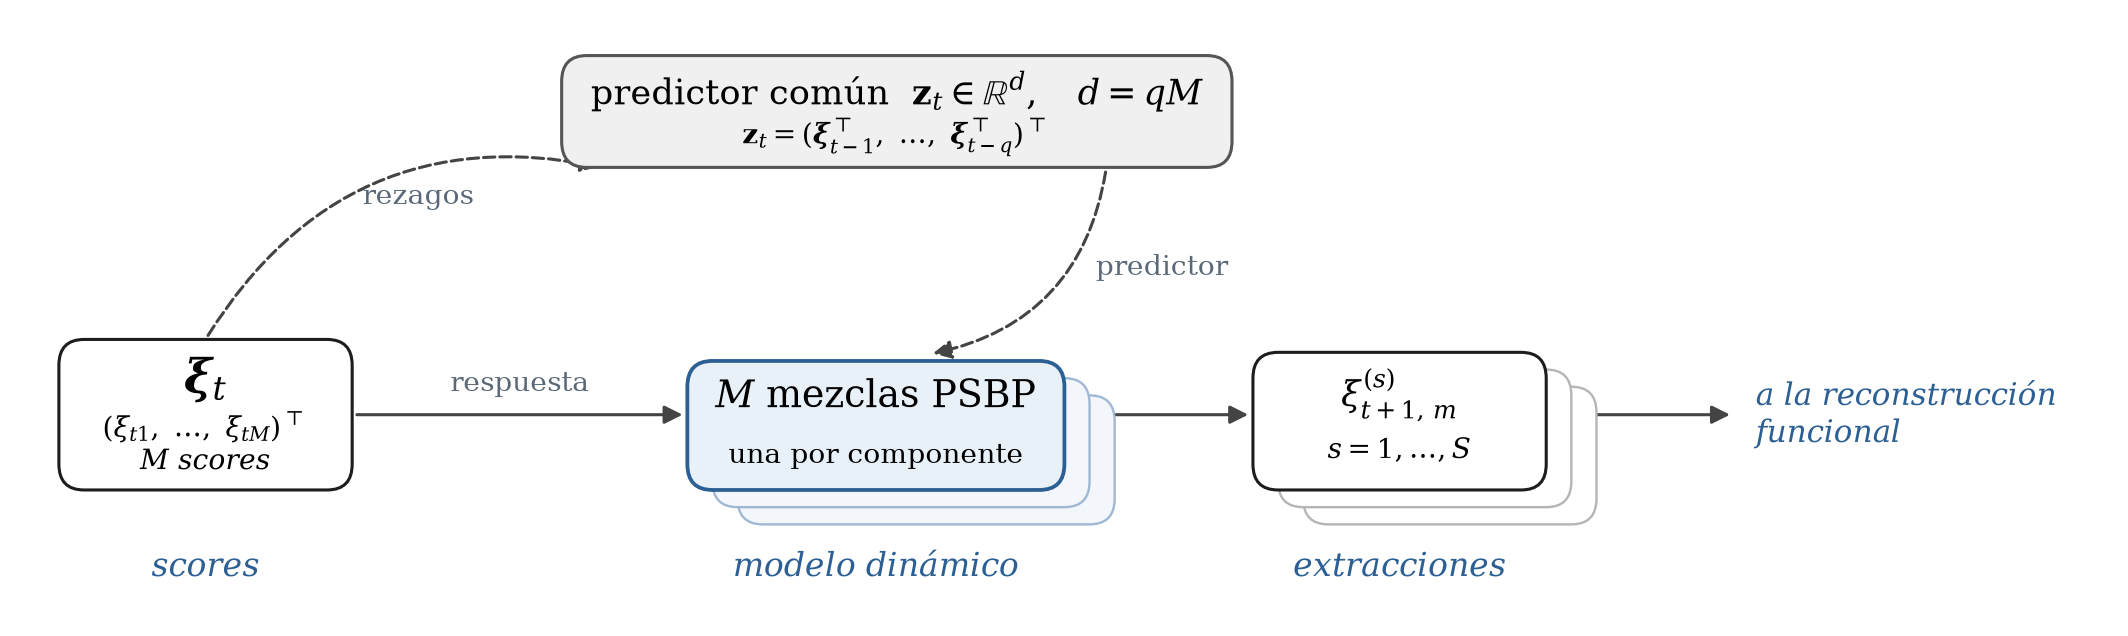
\includegraphics[width=\textwidth]{IMG/03_04/esquema_inferencia_psbpm_fd.png}
    \caption[Esquema de inferencia del PSBPM-FD]{Esquema de inferencia del
    PSBPM-FD. Cada mezcla toma como respuesta el score $\xi_{tm}$ de su
    componente y como predictor el vector común $\mathbf{z}_t$, de modo que el
    rezago de cualquier componente puede influir sobre la ley de cualquier otra.
    Su salida son $S$ extracciones de la predictiva a posteriori.}
    \label{fig:esquema_inferencia_psbpm_fd}
\end{figure}

Sobre estos datos se aplica sin modificación el muestreador de Gibbs descrito en la Sección~\ref{03_03_02_esquema_inferencia_bayesiana}, sustituyendo $y_i$ por $\xi_{tm}$ y $x_i$ por $\mathbf{z}_t$, sobre los $T_0 - q$ pares disponibles en un bloque de entrenamiento de longitud $T_0$. La factorización \eqref{eq:factorizacion} descompone la verosimilitud en el producto de las $M$ verosimilitudes individuales, de manera que los muestreadores son mutuamente independientes.\\

Cada uno entrega una colección de extracciones $\boldsymbol{\Omega}_m^{(s)}$, con $s = 1, \dots, S$, provenientes de la distribución a posteriori $p(\boldsymbol{\Omega}_m \mid \mathcal{D})$ tras descartar el período de calentamiento, donde $\boldsymbol{\Omega}_m$ agrupa los parámetros de pesos y átomos de la $m$-ésima mezcla y $\mathcal{D}$ denota el bloque de entrenamiento. Las extracciones de varias cadenas se agrupan por concatenación. Estas colecciones constituyen la única representación disponible del posterior y son, en consecuencia, el insumo del que se derivan todas las cantidades desconocidas del análisis, que quedan así definidas como funcionales de las extracciones y no como estimaciones puntuales.\\

La primera de dichas cantidades es la distribución predictiva del score, obtenida marginalizando la incertidumbre sobre los parámetros,
\begin{equation}\label{eq:predictiva_posteriori_score}
    f\bigl(\xi_{tm} \mid \mathbf{z}_t, \mathcal{D}\bigr)
    = \int f\bigl(\xi_{tm} \mid \mathbf{z}_t, \boldsymbol{\Omega}_m\bigr)
      p\bigl(\boldsymbol{\Omega}_m \mid \mathcal{D}\bigr) d\boldsymbol{\Omega}_m
    \;\approx\; \frac{1}{S} \sum_{s=1}^{S}
      f\bigl(\xi_{tm} \mid \mathbf{z}_t, \boldsymbol{\Omega}_m^{(s)}\bigr),
\end{equation}
donde el integrando es la mezcla \eqref{eq:psbpm_fd_componente} evaluada en cada extracción. La predictiva es una mezcla de mezclas y no la evaluación de \eqref{eq:psbpm_fd_componente} en una estimación puntual de $\boldsymbol{\Omega}_m$, distinción que resulta determinante para la incertidumbre reportada.\\

La aproximación~\eqref{eq:predictiva_posteriori_score} entrega la densidad predictiva en forma cerrada sobre una grilla, además su versión muestral se obtiene simulando en cada iteración el índice de componente desde la ley de pesos y a continuación la respuesta desde el átomo seleccionado, procedimiento cuya marginal es precisamente~\eqref{eq:predictiva_posteriori_score} y que basta ejecutar una vez por iteración retenida.


\section{Reconstrucción Funcional}
\label{03_05_00_reconstruccion_funcional}

El objeto de interés del estudio no es el score sino la curva, de modo que la predictiva de $\boldsymbol{\xi}_t$ dado $\mathbf{z}_t$, obtenida en $\mathbb{R}^{M}$, debe transportarse al espacio funcional. La descomposición que dio origen a los scores provee esa transformación, ya que la expansión \eqref{eq:expansion_kl_truncada} es un mapa lineal que asigna a cada vector de $\mathbb{R}^{M}$ una curva del subespacio generado por las autofunciones retenidas, y basta recorrerla en sentido inverso al empleado para construir la representación. Proyectando el vector de scores sobre dichas autofunciones, la curva queda escrita como
\begin{equation}\label{eq:reconstruccion_fpca}
    X_t^{(M)}(\tau_g) = \mu(\tau_g)
    + \sum_{m=1}^{M} \xi_{tm}v_m(\tau_g),
    \qquad g = 1, \dots, G,
\end{equation}
donde $\mu(\tau_g)$ y $v_m(\tau_g)$ denotan la función media y las autofunciones evaluadas en la grilla del dominio.\\

La expresión \eqref{eq:reconstruccion_fpca} es una identidad entre el vector de scores y la curva que representa, y adquiere carácter predictivo al evaluarla en el vector aleatorio cuya ley es la predictiva del modelo. Sustituyendo en ella $\boldsymbol{\xi}_t \mid \mathbf{z}_t, \mathcal{D}$ se induce la distribución predictiva de $X_t^{(M)}$ dado el estado rezagado, que es el objeto de interés del pronóstico. Como $\mu(\tau_g)$ y $\{v_m\}$ se tratan como conocidas, el mapa es determinista y afín, propiedad de la que se sigue que los momentos condicionales de la curva se obtengan en forma cerrada a partir de los momentos condicionales de los scores y que cada extracción predictiva de los scores, transportada por el mapa, sea una extracción exacta de la predictiva funcional condicional.\\


La predictiva funcional es por tanto una mezcla, y puede ser multimodal cuando los pesos $\pi_{hm}(\mathbf{z}_t)$ reparten la masa entre átomos de medias separadas; cuántos modos llegan a la curva no se lee de los pesos sino de las extracciones (Sección~\ref{03_06_00_comportamientos}).

\subsection{Esperanza predictiva}
\label{03_05_01_esperanza}

Aplicando el operador esperanza condicional a \eqref{eq:reconstruccion_fpca}, y observando que $\mu(\tau_g)$ y $v_m(\tau_g)$ son constantes que salen del operador, su linealidad entrega
\begin{equation}\label{eq:esperanza_curva}
    \mathbb{E}\bigl[X_t^{(M)}(\tau_g) \mid \mathbf{z}_t, \mathcal{D}\bigr]
    = \mu(\tau_g)
    + \sum_{m=1}^{M} \mathbb{E}\bigl[\xi_{tm} \mid \mathbf{z}_t, \mathcal{D}\bigr]v_m(\tau_g).
\end{equation}
La esperanza predictiva de la curva queda determinada por las $M$ esperanzas predictivas de los scores, sin aproximación adicional.\\

La esperanza de cada score se obtiene de \eqref{eq:predictiva_posteriori_score}. Para una extracción $\boldsymbol{\Omega}_m^{(s)}$, la media de la mezcla es la suma de las medias de sus átomos ponderada por los pesos,
\begin{equation}\label{eq:momento1_iteracion}
    \bar{\mu}_{tm}^{(s)} = \sum_{h=1}^{N} \pi_{hm}^{(s)}\mu_{hm}^{(s)},
    \qquad
    \pi_{hm}^{(s)} = \pi_{hm}\bigl(\mathbf{z}_t; \boldsymbol{\Omega}_m^{(s)}\bigr),
    \quad
    \mu_{hm}^{(s)} = \beta_{0,hm}^{*(s)} + \mathbf{z}_t^\top\boldsymbol{\beta}_{hm}^{*(s)},
\end{equation}
y la esperanza predictiva es el promedio de dichas medias sobre las $S$ extracciones,
\begin{equation}\label{eq:esperanza_score_estimada}
    \widehat{\mathbb{E}}\bigl[\xi_{tm} \mid \mathbf{z}_t, \mathcal{D}\bigr]
    = \frac{1}{S}\sum_{s=1}^{S} \bar{\mu}_{tm}^{(s)}.
\end{equation}
El orden de las operaciones no es intercambiable, ya que $\bar{\mu}_{tm}^{(s)}$ es un funcional de la mezcla completa e invariante a permutaciones de las etiquetas $h$, mientras que los parámetros individuales de cada átomo no lo son.\\


\subsection{Extracciones de la predictiva funcional}
\label{03_05_03_extracciones}

Para cada extracción $s$ de los parámetros y cada componente $m$ se obtiene una extracción del score en dos pasos, primero el índice del átomo, con los pesos evaluados en $\mathbf{z}_t$, y a continuación la respuesta desde el átomo seleccionado,
\begin{equation}\label{eq:extraccion_score}
    h_m^{(s)} \sim \text{Categórica}\Bigl(\pi_{1m}^{(s)}, \dots, \pi_{Nm}^{(s)}\Bigr),
    \qquad
    \xi_{tm}^{(s)} \sim \mathcal{N}\Bigl(\mu_{h_m^{(s)}m}^{(s)},
    \bigl(\nu_{h_m^{(s)}m}^{*(s)}\bigr)^{-1}\Bigr).
\end{equation}
Las $M$ extracciones de una misma iteración $s$ se apilan en un vector, lo que es legítimo bajo la factorización \eqref{eq:factorizacion}, y se transportan a la curva mediante \eqref{eq:reconstruccion_fpca},
\begin{equation}\label{eq:extraccion_curva}
    \widehat{X}_{t}^{(s)}(\tau_g) = \mu(\tau_g)
    + \sum_{m=1}^{M} \xi_{tm}^{(s)}v_m(\tau_g),
    \qquad s = 1, \dots, S.
\end{equation}
Al ser \eqref{eq:reconstruccion_fpca} un mapa determinista, las curvas así construidas son extracciones exactas de la predictiva funcional y la muestra $\{\widehat{X}_t^{(s)}\}_{s=1}^{S}$ es la representación de esa ley. Las curvas se extraen sobre una submuestra equiespaciada de las iteraciones del posterior, una por iteración retenida; en esta sección y en la siguiente, $S$ denota el tamaño de esa submuestra.\\

Al muestrear de este modo, cada extracción elige primero un átomo y luego extrae de él, de manera que la muestra mezcla las extracciones de todos los átomos con peso en $\mathbf{z}_t$ sin registrar de cuál proviene cada una. Si dos o más átomos reciben peso apreciable y sus medias condicionales están separadas, la muestra resulta multimodal y por tanto las extracciones se agrupan en torno a la media de cada átomo. Esa multimodalidad es una propiedad de la mezcla en $\mathbf{z}_t$, no del muestreo, y existiría aunque los parámetros fuesen conocidos. 

\subsection{Predictores puntuales de la curva}
\label{03_05_04_predictores_puntuales}

La esperanza de la Sección~\ref{03_05_01_esperanza} es el predictor puntual óptimo bajo pérdida cuadrática cualquiera sea la forma de la predictiva, y describe bien lo que el modelo espera cuando esta es unimodal y simétrica, por ejemplo cuando los pesos $\pi_{hm}(\mathbf{z}_t)$ concentran la masa en un solo átomo. Cuando la predictiva resulta multimodal o asimétrica, lo que suele indicar que el estado rezagado $\mathbf{z}_t$ no separa por completo los regímenes de la mezcla, la esperanza pasa a ser un promedio de comportamientos posibles que no coincide con ninguno de ellos. Por eso se presentan dos predictores menos sensibles a esos efectos, calculados sobre las extracciones de la Sección~\ref{03_05_03_extracciones}.
 

\subsubsection{Mediana puntual}
\label{03_05_04_01_mediana_puntual}

Denotando por $\widehat{F}_{t,g}$ la función de distribución empírica de la muestra en el punto $\tau_g$,
\begin{equation}\label{eq:fdist_empirica}
    \widehat{F}_{t,g}(y) = \frac{1}{S}\sum_{s=1}^{S}
    \mathbf{1}\bigl\{\widehat{X}_{t}^{(s)}(\tau_g) \leq y\bigr\},
\end{equation}
la mediana puntual es la curva $\widehat{X}_t^{\mathrm{med}}(\tau_g) = \widehat{F}_{t,g}^{-1}(1/2)$. Como el error absoluto funcional es una integral de errores absolutos en cada punto, la mediana puntual lo minimiza punto a punto y es el predictor consistente con esa métrica. Su limitación es que no es necesariamente una curva que el modelo genere, ya que en cada punto del dominio toma la mediana de las extracciones, y si en una parte del dominio domina un grupo de extracciones y en otra parte domina otro, el resultado junta tramos de curvas distintas. 

\subsubsection{Átomo más probable}
\label{03_05_04_02_atomo_modal}
 En cada iteración $s$ y componente $m$ se toma el átomo de mayor peso en $\mathbf{z}_t$ y su media condicional,
\begin{equation}\label{eq:atomo_modal}
    h_m^{\star(s)} = \operatorname*{argmax}_{h} \pi_{hm}^{(s)},
    \qquad
    \xi_{tm}^{\mathrm{mod}} = \operatorname{mediana}_{s}\mu_{h_m^{\star(s)} m}^{(s)},
\end{equation}
y la curva modal se obtiene transportando el vector $\boldsymbol{\xi}_t^{\mathrm{mod}}$ por \eqref{eq:reconstruccion_fpca}. Se trata, en cada iteración, del predictor óptimo bajo pérdida cero-uno sobre la asignación de régimen de cada componente, y su cálculo es exacto, ya que la ley conjunta de los $M$ scores es una mezcla sobre configuraciones $(h_1, \dots, h_M)$ con pesos $\prod_m \pi_{h_m m}^{(s)}$, de modo que, al maximizarse un producto de factores independientes factor a factor, la configuración más probable es la que toma el átomo más probable de cada componente. La agregación sobre $s$ se realiza mediante la mediana y no mediante el promedio, con el fin de evitar que las iteraciones en que los pesos $\pi_{hm}^{(s)}$ se reparten casi por igual entre dos átomos desplacen el predictor hacia la región entre ambos. Este predictor responde a cómo sería la curva si se realizara el régimen más probable y acompaña de modo natural a la probabilidad de ese régimen.\\

Los tres predictores coinciden aproximadamente cuando la predictiva es unimodal y simétrica, y se separan en la medida en que no lo es. 

\subsection{Intervalos de credibilidad predictivos}
\label{03_05_05_intervalos_predictivos}

Los intervalos se construyen a partir de los cuantiles empíricos de las extracciones y no como intervalos simétricos en torno a la esperanza, que impondrían por construcción la simetría y unimodalidad que el modelo existe para no suponer.\\


\subsubsection{Intervalo puntual equi-colas}
\label{03_05_05_01_equicolas}
Con la distribución empírica \eqref{eq:fdist_empirica}, el intervalo de credibilidad de nivel $1-\zeta$ en cada punto del dominio es
\begin{equation}\label{eq:intervalo_puntual}
    \Bigl[\widehat{F}_{t,g}^{-1}(\zeta/2),\;
    \widehat{F}_{t,g}^{-1}(1-\zeta/2)\Bigr],
    \qquad g = 1, \dots, G.
\end{equation}
El intervalo así construido es puntual y no simultáneo.

\subsubsection{Banda simultánea}
\label{03_05_05_02_banda_simultanea}
Cuando el objeto de interés es la curva completa, la banda debe calibrarse para que contenga la curva entera con probabilidad $1-\zeta$. Con la mediana puntual como centro $\widehat{X}_t^{\mathrm{med}}(\tau_g)$ y como escala $\widehat{\sigma}_t(\tau_g)$ el rango intercuartílico de la muestra dividido por $1.349$, ambos robustos frente a las colas no acotadas de los átomos cuando $a_\nu \le 1$, se define la desviación máxima normalizada de cada extracción,
\begin{equation}\label{eq:supnorma}
    D^{(s)} = \max_{g}\;\frac{\bigl|\widehat{X}_t^{(s)}(\tau_g) - \widehat{X}_t^{\mathrm{med}}(\tau_g)\bigr|}{\widehat{\sigma}_t(\tau_g)},
\end{equation}
y la banda $\widehat{X}_t^{\mathrm{med}}(\tau_g) \pm q_{1-\zeta}(D)\widehat{\sigma}_t(\tau_g)$, con $q_{1-\zeta}(D)$ el cuantil empírico de $\{D^{(s)}\}$, contiene por construcción a una fracción $1-\zeta$ de las extracciones en toda su extensión. Es la banda de tipo supremo de \citet{03_05_degras2011bands} evaluada sobre la predictiva. Esta banda tiene una limitación cuando la predictiva es multimodal, porque al ser una región conexa cubre también el valle entre las cumbres.

\subsubsection{Región de máxima densidad}
\label{03_05_05_03_hdr}

La región de máxima densidad de nivel $1-\zeta$ \citep{03_05_hyndman1996hdr} es el conjunto de menor medida que acumula probabilidad $1-\zeta$,
\begin{equation}\label{eq:hdr}
    \mathcal{R}_{1-\zeta} = \bigl\{y : f(y) \geq f_{\zeta}\bigr\},
    \qquad
    \Pr\bigl(Y \in \mathcal{R}_{1-\zeta}\bigr) = 1-\zeta,
\end{equation}
con $f$ la densidad predictiva. Con una predictiva unimodal y simétrica coincide con el intervalo equi-colas, mientras que con dos modos separados por un valle cuya densidad cae bajo $f_\zeta$ es la unión de dos intervalos, uno por modo, cuya longitud total es menor que la del intervalo central al mismo nivel porque excluye el valle. Es la contraparte, para intervalos, de la observación de la Sección~\ref{03_05_04_predictores_puntuales} sobre la esperanza.\\

En el caso funcional la región se construye punto a punto sobre el dominio, del mismo modo que el intervalo \eqref{eq:intervalo_puntual}. En cada $\tau_g$ se estima por núcleo la densidad de la muestra $\{\widehat{X}_t^{(s)}(\tau_g)\}_{s=1}^{S}$ y se toma el conjunto \eqref{eq:hdr}, que donde la predictiva es unimodal y simétrica coincide con el intervalo equi-colas y donde es multimodal puede descomponerse en varios tramos.\\

El puntaje de Winkler se extiende a una región de este tipo sumando las longitudes de sus tramos y penalizando por la distancia de la observación al tramo más cercano, y del mismo modo el MPIW suma las longitudes de los tramos y el PICP cuenta si la observación cae en alguno de ellos, de manera que las tres construcciones se comparan con las métricas de la Sección~\ref{02_02_03_criterios_evaluacion}. Cabe tener presente que el funcional que el puntaje de Winkler elicita es el intervalo central, de modo que la región de máxima densidad no tiene por qué mejorarlo aun cuando sea más angosta.

\section{Comportamientos predictivos}
\label{03_06_00_comportamientos}
En cada iteración, la predictiva conjunta de los scores es una mezcla sobre configuraciones de átomos $(h_1, \dots, h_M)$ con pesos $\prod_m \pi_{h_m m}^{(s)}$, y la forma que toma depende de cuánto informa el estado rezagado $\mathbf{z}_t$ sobre el régimen. Si lo determina, los pesos concentran la masa en átomos de un mismo régimen y la predictiva tiene un solo modo, si no lo determina, la masa se reparte entre átomos de regímenes distintos, y por tanto la predictiva tiene un modo por cada uno. A cada uno de esos modos se le llama comportamiento predictivo.\\

Los comportamientos se identifican origen por origen, como parte de la predicción de cada curva, y de cada uno se obtienen su probabilidad, su curva típica y su dispersión. Así pueden contrastarse con los regímenes del proceso cuando se conocen, o con una variable que los represente cuando no. Los modelos de referencia, cuya predictiva es unimodal, no admiten esta descomposición.\\

Los comportamientos no pueden leerse de los parámetros, ya que los átomos de componentes distintas no se corresponden entre sí, un mismo régimen puede repartirse en varios átomos equivalentes y el peso de una configuración completa, al ser un producto de $M$ pesos, no se interpreta como la probabilidad de un comportamiento. Lo único que vincula a las $M$ mezclas es $\mathbf{z}_t$, de modo que los comportamientos se identifican sobre las extracciones, que son extracciones de la predictiva conjunta en ese $\mathbf{z}_t$. 
 
\subsection{Agrupamiento de las extracciones}
\label{03_06_01_agrupamiento}

Como las autofunciones son ortonormales en $L^2$, la distancia euclídea entre dos vectores de scores coincide con la distancia $L^2$ entre las curvas que representan, de modo que basta agrupar las extracciones en $\mathbb{R}^{M}$ con los scores. Para cada origen $t$ se agrupan las $S$ extracciones $\{\boldsymbol{\xi}_t^{(s)}\}$ mediante $k$-medias, esto es, se busca la partición en $K$ grupos $\mathcal{G}_1, \dots, \mathcal{G}_K$ que minimiza la suma de cuadrados dentro de los grupos,
\begin{equation}\label{eq:kmedias}
    \min_{\mathcal{G}_1, \dots, \mathcal{G}_K}\ \sum_{k=1}^{K}\ \sum_{s \in \mathcal{G}_k} \bigl\lVert \boldsymbol{\xi}_t^{(s)} - \bar{\boldsymbol{\xi}}_{t,k} \bigr\rVert^{2},
    \qquad
    \bar{\boldsymbol{\xi}}_{t,k} = \frac{1}{\lvert \mathcal{G}_k \rvert}\sum_{s \in \mathcal{G}_k} \boldsymbol{\xi}_t^{(s)},
\end{equation}
resuelta alternando la asignación de cada extracción al centroide más cercano con el recálculo de los centroides como medias de sus grupos, desde varios inicios aleatorios.\\

La fracción de varianza explicada por la partición, $R^2_K = 1 - \mathrm{SCD}_K / \mathrm{SCD}_1$ con $\mathrm{SCD}_K$ el mínimo de \eqref{eq:kmedias}, crece con $K$ aunque no exista estructura, de manera que el número de comportamientos no puede fijarse por un umbral sobre ella y se decide con las tres reglas de la Sección~\ref{03_06_02_numero}. Cuando la distribución a priori de las precisiones admite átomos de varianza no acotada, las extracciones se recortan a los cuantiles extremos de cada score antes del agrupamiento.

\subsection{Número de comportamientos}
\label{03_06_02_numero}

La primera regla decide si existe más de un comportamiento. Con $K = 2$, las extracciones se proyectan sobre el eje que une los dos centroides, $\mathbf{d}_t = (\bar{\boldsymbol{\xi}}_{t,2} - \bar{\boldsymbol{\xi}}_{t,1}) / \lVert \bar{\boldsymbol{\xi}}_{t,2} - \bar{\boldsymbol{\xi}}_{t,1} \rVert$, y sobre la proyección se estima por núcleo la densidad $\widehat{f}$. Se declara que hay dos modos si la densidad entre los centroides desciende por debajo de la mitad de la menor de las densidades evaluadas en ellos,
\begin{equation}\label{eq:valle}
    \frac{\min_{x_1 \le x \le x_2} \widehat{f}(x)}{\min\bigl\{\widehat{f}(x_1), \widehat{f}(x_2)\bigr\}} < \tfrac{1}{2},
    \qquad x_1 = \bar{\boldsymbol{\xi}}_{t,1}^\top \mathbf{d}_t,\ \ x_2 = \bar{\boldsymbol{\xi}}_{t,2}^\top \mathbf{d}_t,
\end{equation}
y en caso contrario se declara un único comportamiento. Esta regla es una versión operativa del contraste de unimodalidad de \citet{03_05_hartigan1985dip}, y es la que distingue una predictiva con dos modos de una unimodal alargada o asimétrica, que $k$-medias también parte en dos pero sin que la densidad presente un valle.\\

La segunda regla acota el número de comportamientos. A partir de $K = 2$ se acepta la partición en $K + 1$ grupos solo si el grupo adicional explica al menos tanto como explica en promedio cada uno de los existentes,
\begin{equation}\label{eq:crecimiento}
    R^2_{K+1} \;\geq\; R^2_K + \frac{R^2_K}{K},
\end{equation}
condición equivalente a que la varianza explicada por comportamiento no disminuya, y el barrido se detiene en el primer $K$ que la incumple.\\

La tercera regla exige que cada comportamiento reúna una masa de al menos $\zeta$, el nivel de la banda de credibilidad, de manera que un comportamiento sea un grupo de extracciones que la banda al nivel $1-\zeta$ tendría que cubrir; un grupo de masa menor es una cola y no un comportamiento, y la partición que lo produce se descarta. Las tres reglas dependen de dos constantes, el cociente de valle y $\zeta$.

\subsection{Probabilidad, curva típica, pronóstico por comportamiento y su cota}
\label{03_06_03_descripcion}

El resultado por origen es un conjunto de $K_t$ comportamientos. Cada uno tiene probabilidad $p_{t,k} = \lvert \mathcal{G}_k \rvert / S$, igual a la fracción de extracciones del grupo, curva típica $\widehat{X}_{t,k}$ igual al centroide $\bar{\boldsymbol{\xi}}_{t,k}$ transportado por \eqref{eq:reconstruccion_fpca}, que por linealidad del mapa es la esperanza predictiva condicional a ese comportamiento, e intervalo condicional dado por los cuantiles equi-colas \eqref{eq:intervalo_puntual} calculados solo sobre las extracciones del grupo. La mezcla de las curvas típicas ponderada por sus probabilidades es la media de las extracciones recortadas, que aproxima a la esperanza predictiva de la Sección~\ref{03_05_01_esperanza},
\begin{equation}\label{eq:esperanza_por_comportamientos}
    \widehat{\mathbb{E}}\bigl[X_t^{(M)}(\tau_g) \mid \mathbf{z}_t, \mathcal{D}\bigr]
    \approx \sum_{k=1}^{K_t} p_{t,k}\widehat{X}_{t,k}(\tau_g),
\end{equation}
relación que muestra por qué, con más de un comportamiento, la esperanza se sitúa entre ellos. El contraste entre dos comportamientos es la diferencia de sus curvas típicas, $\Delta_{t,kk'}(\tau_g) = \widehat{X}_{t,k}(\tau_g) - \widehat{X}_{t,k'}(\tau_g)$, que localiza en qué parte del dominio difieren y en cuánto.\\

Los comportamientos permiten un predictor puntual distinto de los de la Sección~\ref{03_05_04_predictores_puntuales}. Aquellos resumen la predictiva completa, y por \eqref{eq:esperanza_por_comportamientos} la esperanza queda entre los comportamientos cuando hay más de uno, mientras que la mediana puntual elige entre modos de forma indirecta y el átomo más probable lo hace componente a componente en el espacio de los scores. El pronóstico por comportamiento elige de forma explícita un modo de la predictiva conjunta, ya que se toma el comportamiento de mayor probabilidad y se predice con su curva típica,
\begin{equation}\label{eq:pronostico_comportamiento}
    \widehat{X}_t^{\mathrm{mp}}(\tau_g) = \widehat{X}_{t,k_t^{*}}(\tau_g),
    \qquad
    k_t^{*} = \arg\max_{k = 1, \ldots, K_t} p_{t,k}.
\end{equation}
Con $K_t = 1$ se toma la esperanza predictiva de la Sección~\ref{03_05_01_esperanza}, de modo que el predictor solo se aparta de ella en los orígenes en que la predictiva tiene más de un modo, y ahí lo hace comprometiéndose con uno de ellos en lugar de promediarlos. Del mismo modo, es natural extender a cada comportamiento los otros dos predictores de la Sección~\ref{03_05_04_predictores_puntuales}, la mediana puntual y el átomo más probable, calculados solo sobre las extracciones del comportamiento elegido (y, con $K_t = 1$, sobre la predictiva completa); la mediana puntual es la variante del mismo predictor para una condicional asimétrica.\\

El pronóstico \eqref{eq:pronostico_comportamiento} es una regla de elección entre los $K_t$ comportamientos, y conviene separar lo que pierde por elegir de lo que la predictiva no contiene. Para eso se define su cota, el mejor comportamiento, como la curva típica del comportamiento más cercano en $L^2$ a la curva observada,
\begin{equation}\label{eq:mejor_comportamiento}
    \widehat{X}_t^{\mathrm{cota}}(\tau_g) = \widehat{X}_{t,k_t^{\circ}}(\tau_g),
    \qquad
    k_t^{\circ} = \arg\min_{k = 1, \ldots, K_t} \bigl\lVert X_t - \widehat{X}_{t,k} \bigr\rVert,
\end{equation}
que con $K_t = 1$ coincide con el pronóstico. No es un predictor, porque elige con la observación, sino una cota, el menor error que puede alcanzar cualquier regla que pronostique con uno de los comportamientos. La distancia entre el pronóstico y su cota mide lo que cuesta elegir con la probabilidad en vez de con la curva observada, y la distancia entre la cota y la esperanza, cuánto hay que ganar si se eligiera bien. Además permite ver si la curva que ocurre está entre las opciones que la predictiva entrega, de modo que, cuando la cota queda por debajo de las referencias y el pronóstico no, la desventaja está en resumir la predictiva en una curva y no en la información que contiene.


\section{Diseño del Estudio de Simulación}
\label{03_07_00_diseno_estudio_simulacion}

El estudio aborda tres preguntas de evaluación: ¿en cuáles de los tres escenarios la predicción puntual del PSBPM-FD supera a la de los modelos de referencia?, ¿en cuáles sus intervalos de credibilidad ofrecen un mejor desempeño? y, en el escenario con cambio de régimen, ¿en qué medida los comportamientos de su distribución predictiva reproducen los regímenes del proceso y permiten generar pronósticos a partir de ellos? La evaluación se realiza mediante las métricas definidas en la Sección~\ref{02_02_03_criterios_evaluacion}.\\

En los tres escenarios el procedimiento es el mismo, las curvas se generan con el esquema común del Anexo~\ref{ane_00_01_esquema_comun} y se parten en orden cronológico en un bloque de entrenamiento ($70\%$) y uno de prueba. Las predicciones a un paso sobre el segundo usan los rezagos observados, sin reestimar.\\

Las métricas de la Sección~\ref{02_02_03_criterios_evaluacion} se calculan sobre la ventana móvil de ancho $w_{\mathrm{ref}} = 30$, contra la curva ajustada por la representación (Sección~\ref{03_05_00_reconstruccion_funcional}), para cada $M$ del barrido. El PSBPM-FD se ajusta con los hiperparámetros de \citet{03_02_chung2009nonparametric} llevados a la escala de cada score.\\

Las referencias son el FAR, con orden fijo igual al número de rezagos del escenario e intervalo gaussiano, y el Random Forest con la misma especificación que el PSBPM-FD. Se reportan el MAE y el RMSE de los tres predictores puntuales, del pronóstico por comportamiento (Sección~\ref{03_06_03_descripcion}) y de su cota \eqref{eq:mejor_comportamiento}, estos dos solo en C-2, cada uno contra el FAR y el Random Forest; y el Winkler, el MPIW y el PICP de las tres construcciones de intervalo contra el FAR.\\

Los comportamientos predictivos y el pronóstico que se construye con ellos se evalúan solo en C-2, el escenario cuya ley condicional reparte su masa entre regímenes separados. En C-1 la media condicional es única y en C-3 la multimodalidad queda en la ley conjunta de los scores y no llega a la marginal de cada score ni a la de la curva, de modo que en ambos se espera que la predictiva tenga un solo comportamiento y el pronóstico por comportamiento coincida con la esperanza, lo que la Sección~\ref{03_08_03_comportamientos} confirma. En C-2 los comportamientos se resumen por la distribución de $K_t$ en el bloque de prueba y, origen a origen, en una ventana de detalle de $N_{\mathrm{det}} = 10$ orígenes consecutivos, la de más cambios de régimen verdadero, elegida con lo que el generador registra y nunca con lo predicho. La configuración completa está en el Anexo~\ref{ane_00_03_configuracion} y las métricas restantes y los otros anchos de ventana, en el Anexo~\ref{aneB_00_00_resultados_simulacion}.

\subsection{Escenarios}
\label{03_07_02_escenarios}

Cada escenario introduce un rasgo de la ley condicional del score que un modelo de media lineal no representa; los algoritmos y sus valores están en el Anexo~\ref{ane_00_00_anexo}. En los tres la dinámica vive en los $J_a = 4$ primeros scores y los restantes son autorregresivos de primer orden, de modo que $M = 4$ es la primera dimensión que observa toda la dinámica.\\

El régimen o mecanismo que sortea el generador se registra pero no se entrega a ningún método. El Cuadro~\ref{tab:dis_escenarios} resume la configuración de cada escenario, con $q$ el número de rezagos. Con rezagos propios, la mezcla de la componente $m$ recibe solo $(\xi_{t-1,m}, \dots, \xi_{t-q,m})^\top$, la restricción de $\mathbf{z}_t$ a sus propios rezagos, de modo que $d = q$; con los rezagos de todas las componentes, $d = qM$.

\begin{table}[H]
\centering\small
\setlength{\tabcolsep}{4pt}
\caption{Escenarios del estudio y configuración de los métodos en cada uno.}
\label{tab:dis_escenarios}
\begin{tabular}{p{0.07\textwidth} p{0.30\textwidth} p{0.14\textwidth} p{0.05\textwidth} p{0.20\textwidth} p{0.10\textwidth}}
\hline
 & Rasgo & Algoritmo & $q$ & Covariables & $M$ \\
\hline
C-1 & Heterocedasticidad condicional        & Anexo~\ref{ane_00_02_01_alg_c1} & $4$ & Rezagos propios                       & $1,\ldots,10$ \\
C-2 & Cambio de régimen por umbral          & Anexo~\ref{ane_00_02_02_alg_c2} & $4$ & Rezagos propios                       & $1,\ldots,10$ \\
C-3 & Multimodalidad en la ley conjunta de los scores & Anexo~\ref{ane_00_02_03_alg_c3} & $2$ & Rezagos de todas las componentes & $3,\ldots,6$ \\
\hline
\end{tabular}
\end{table}

\begin{itemize}
    \item \textbf{C-1.} Los scores activos son autorregresivos con innovaciones GARCH$(1,1)$. La media condicional es lineal y la no linealidad está únicamente en la varianza, con una memoria de unas siete curvas. Como la señal de volatilidad depende de los dos rezagos propios más próximos, el modelo puede aprenderla, por lo que la ventaja esperable del PSBPM-FD está en los intervalos de credibilidad y no en la predicción puntual.

    \item \textbf{C-2.} Cada score activo alterna, mediante una transición probit dependiente de su propio rezago, entre un régimen persistente de escala pequeña y otro más volátil y con reversión. La media condicional es no lineal y la varianza depende del estado. La calibración favorece deliberadamente la separación entre regímenes, por lo que las conclusiones se limitan a esta configuración.

       \item \textbf{C-3.} Un softmax sobre los dos rezagos de los dos primeros scores selecciona entre tres mecanismos lineales, uno central y dos con niveles distintos, cuyas localizaciones difieren en más que la escala de la innovación. Esto genera una ley condicional multimodal en el espacio conjunto de los scores, aunque la media condicional sea casi lineal y la marginal de cada score quede casi unimodal. Como el mecanismo depende de los rezagos de $\xi_1$ y $\xi_2$, las covariables incluyen los rezagos de todas las componentes y el muestreador se ejecuta para cada valor de $M$.
\end{itemize}


\section{Resultados}
\label{03_08_00_resultados}

Cada apartado de esta sección responde a una de las preguntas del diseño con la misma lectura en tres niveles, el promedio sobre las ventanas de prueba para cada $M$ del barrido, la fracción de ventanas que gana cada modelo en $M_{\mathrm{ref}}$, y la trayectoria de la métrica a lo largo del bloque de prueba, de modo que una diferencia en el promedio pueda atribuirse a una ventaja sostenida o a unos pocos tramos.\\

Todas las cifras son contra la curva ajustada por la representación, con la ventana de ancho $w_{\mathrm{ref}} = 30$ y, salvo indicación, con $M_{\mathrm{ref}} = 10$ en C-1 y C-2 y $M_{\mathrm{ref}} = 6$ en C-3. La Sección~\ref{03_08_01_error_puntual} compara los tres predictores puntuales del PSBPM-FD con el FAR y el Random Forest, la Sección~\ref{03_08_02_intervalos} hace lo propio con las tres construcciones de intervalo frente a la banda gaussiana del FAR, y las Secciones~\ref{03_08_03_comportamientos} y~\ref{03_08_04_pronostico}, restringidas a C-2, examinan cuántos comportamientos declara la predictiva, cómo se comparan con los de la ley verdadera y qué se gana y se pierde al pronosticar con el más probable.


\subsection{Error puntual}
\label{03_08_01_error_puntual}

Los Cuadros~\ref{tab:res_bloqueA} y~\ref{tab:res_bloqueA_rmse} resumen el MAE y el RMSE promedio sobre las ventanas de prueba, contra la curva ajustada, de los tres predictores puntuales del PSBPM-FD y de las dos referencias, para cada $M$ del barrido. Las Figuras~\ref{fig:res_bloqueA_vs_M_C1} a~\ref{fig:res_bloqueA_vs_M_C3} muestran las mismas cifras contra $M$ y el Cuadro~\ref{tab:res_bloqueA_ventanas}, en $M_{\mathrm{ref}}$, cómo se reparten las ventanas entre los modelos.

\begin{table}[H]
\centering\small
\setlength{\tabcolsep}{3.5pt}
\caption{MAE en el bloque de prueba por escenario y $M$. En negrita el menor en $M_{\mathrm{ref}}$.}
\label{tab:res_bloqueA}
\begin{tabular}{c cccc cccc cccc}
\hline
 & \multicolumn{4}{c}{C-1} & \multicolumn{4}{c}{C-2} & \multicolumn{4}{c}{C-3} \\
$M$ & Esp. & Med. & Modal & RF & Esp. & Med. & Modal & RF & Esp. & Med. & Modal & RF \\
\hline
$1$  & 0.754 & 0.755 & 0.755 & 0.764 & 0.714 & 0.720 & 0.725 & 0.710 & --- & --- & --- & --- \\
$2$  & 0.739 & 0.739 & 0.739 & 0.753 & 0.673 & 0.675 & 0.691 & 0.658 & --- & --- & --- & --- \\
$3$  & 0.724 & 0.724 & 0.726 & 0.740 & 0.635 & 0.633 & 0.652 & 0.617 & 0.694 & 0.695 & 0.703 & 0.699 \\
$4$  & 0.716 & 0.717 & 0.722 & 0.734 & 0.612 & 0.605 & 0.635 & 0.591 & 0.689 & 0.691 & 0.700 & 0.699 \\
$5$  & 0.714 & 0.714 & 0.719 & 0.733 & 0.610 & 0.603 & 0.633 & 0.591 & 0.684 & 0.685 & 0.693 & 0.693 \\
$6$  & 0.713 & 0.713 & 0.718 & 0.732 & 0.609 & 0.602 & 0.632 & 0.592 & \textbf{0.689} & 0.689 & 0.698 & 0.700 \\
$7$  & 0.712 & 0.713 & 0.718 & 0.733 & 0.609 & 0.601 & 0.631 & 0.592 & --- & --- & --- & --- \\
$8$  & 0.712 & 0.712 & 0.717 & 0.733 & 0.609 & 0.601 & 0.631 & 0.592 & --- & --- & --- & --- \\
$9$  & 0.711 & 0.712 & 0.717 & 0.734 & 0.609 & 0.601 & 0.631 & 0.591 & --- & --- & --- & --- \\
$10$ & \textbf{0.711} & 0.712 & 0.717 & 0.734 & 0.609 & 0.601 & 0.631 & \textbf{0.591} & --- & --- & --- & --- \\
\hline
FAR & \multicolumn{4}{c}{0.723} & \multicolumn{4}{c}{0.770} & \multicolumn{4}{c}{0.700} \\
\hline
\end{tabular}
\end{table}

% Fuente: 98_resumen_bloqueA_min_max_prom.csv del _05 (test, rmse_f).
\begin{table}[H]
\centering\small
\setlength{\tabcolsep}{3.5pt}
\caption{RMSE en el bloque de prueba por escenario y $M$. En negrita el menor en $M_{\mathrm{ref}}$.}
\label{tab:res_bloqueA_rmse}
\begin{tabular}{c cccc cccc cccc}
\hline
 & \multicolumn{4}{c}{C-1} & \multicolumn{4}{c}{C-2} & \multicolumn{4}{c}{C-3} \\
$M$ & Esp. & Med. & Modal & RF & Esp. & Med. & Modal & RF & Esp. & Med. & Modal & RF \\
\hline
$1$  & 0.951 & 0.953 & 0.953 & 0.967 & 0.906 & 0.920 & 0.927 & 0.906 & --- & --- & --- & --- \\
$2$  & 0.923 & 0.924 & 0.925 & 0.943 & 0.854 & 0.865 & 0.889 & 0.843 & --- & --- & --- & --- \\
$3$  & 0.903 & 0.904 & 0.908 & 0.927 & 0.808 & 0.816 & 0.849 & 0.793 & 0.870 & 0.872 & 0.880 & 0.878 \\
$4$  & 0.895 & 0.897 & 0.905 & 0.922 & 0.783 & 0.787 & 0.839 & 0.767 & 0.866 & 0.868 & 0.882 & 0.877 \\
$5$  & 0.893 & 0.894 & 0.903 & 0.921 & 0.781 & 0.783 & 0.837 & 0.766 & 0.860 & 0.861 & 0.872 & 0.870 \\
$6$  & 0.891 & 0.892 & 0.902 & 0.920 & 0.779 & 0.781 & 0.835 & 0.766 & \textbf{0.866} & 0.866 & 0.879 & 0.877 \\
$7$  & 0.891 & 0.892 & 0.901 & 0.920 & 0.778 & 0.780 & 0.834 & 0.766 & --- & --- & --- & --- \\
$8$  & 0.890 & 0.891 & 0.901 & 0.920 & 0.777 & 0.779 & 0.834 & 0.766 & --- & --- & --- & --- \\
$9$  & 0.890 & 0.891 & 0.901 & 0.920 & 0.777 & 0.779 & 0.833 & 0.766 & --- & --- & --- & --- \\
$10$ & \textbf{0.890} & 0.891 & 0.901 & 0.920 & 0.777 & 0.779 & 0.833 & \textbf{0.766} & --- & --- & --- & --- \\
\hline
FAR & \multicolumn{4}{c}{0.906} & \multicolumn{4}{c}{0.980} & \multicolumn{4}{c}{0.880} \\
\hline
\end{tabular}
\end{table}

% Figura Bloque A contra M: MAE y RMSE de los tres predictores, FAR y RF. Fuente: 98_* del _05.
\begin{figure}[H]
\centering
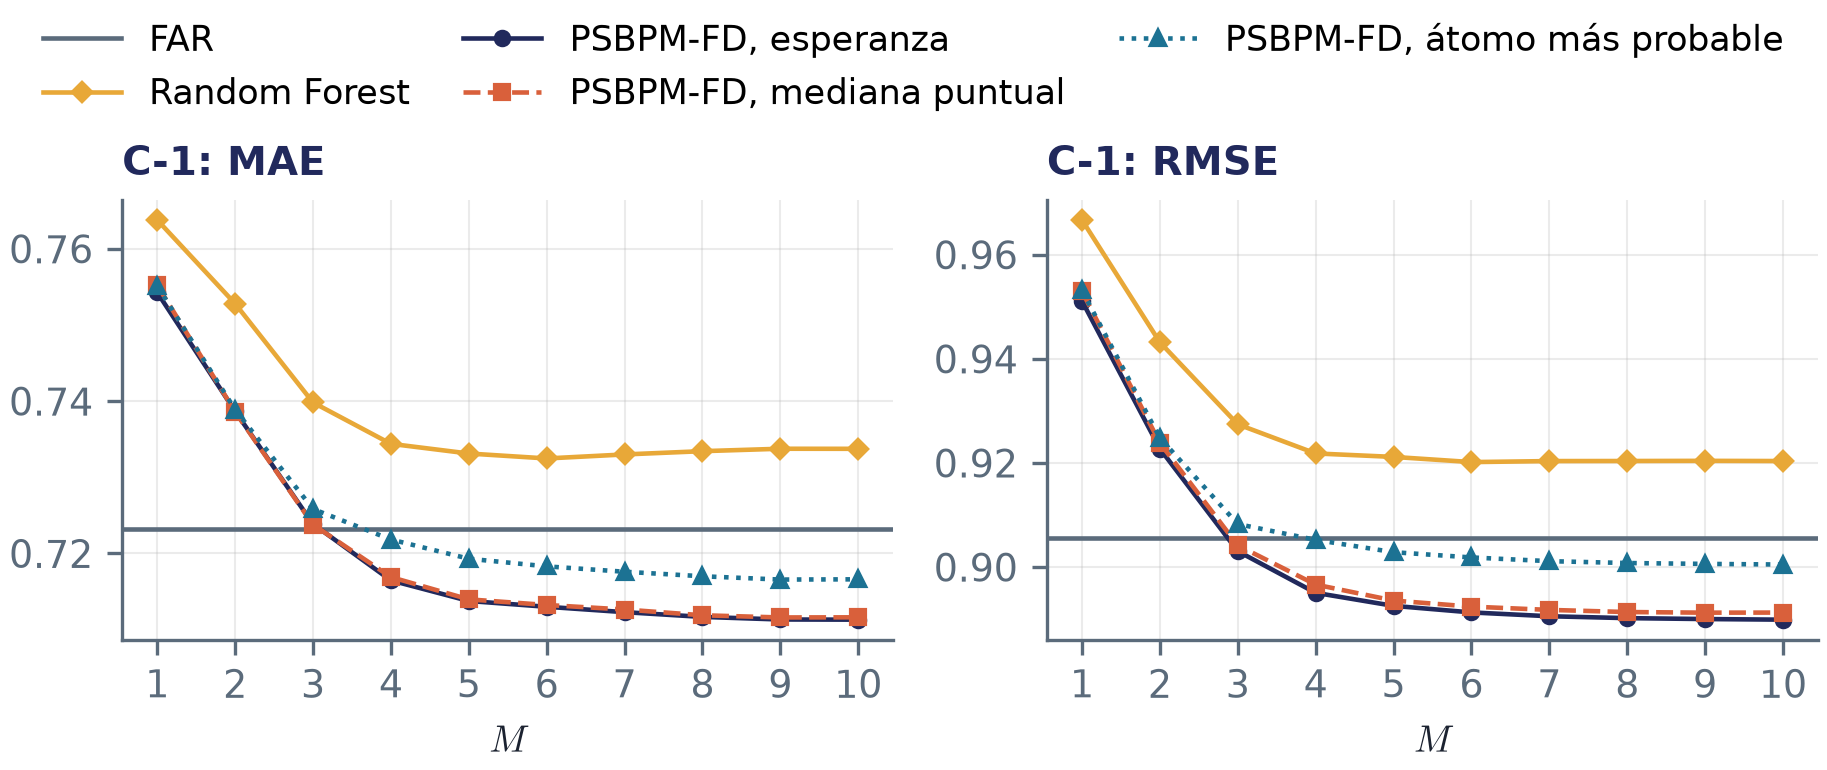
\includegraphics[width=\textwidth]{IMG/03_08/03_08_bloqueA_vs_M_C1.png}
\caption{C-1. MAE y RMSE en el bloque de prueba contra $M$.}
\label{fig:res_bloqueA_vs_M_C1}
\end{figure}

\begin{figure}[H]
\centering
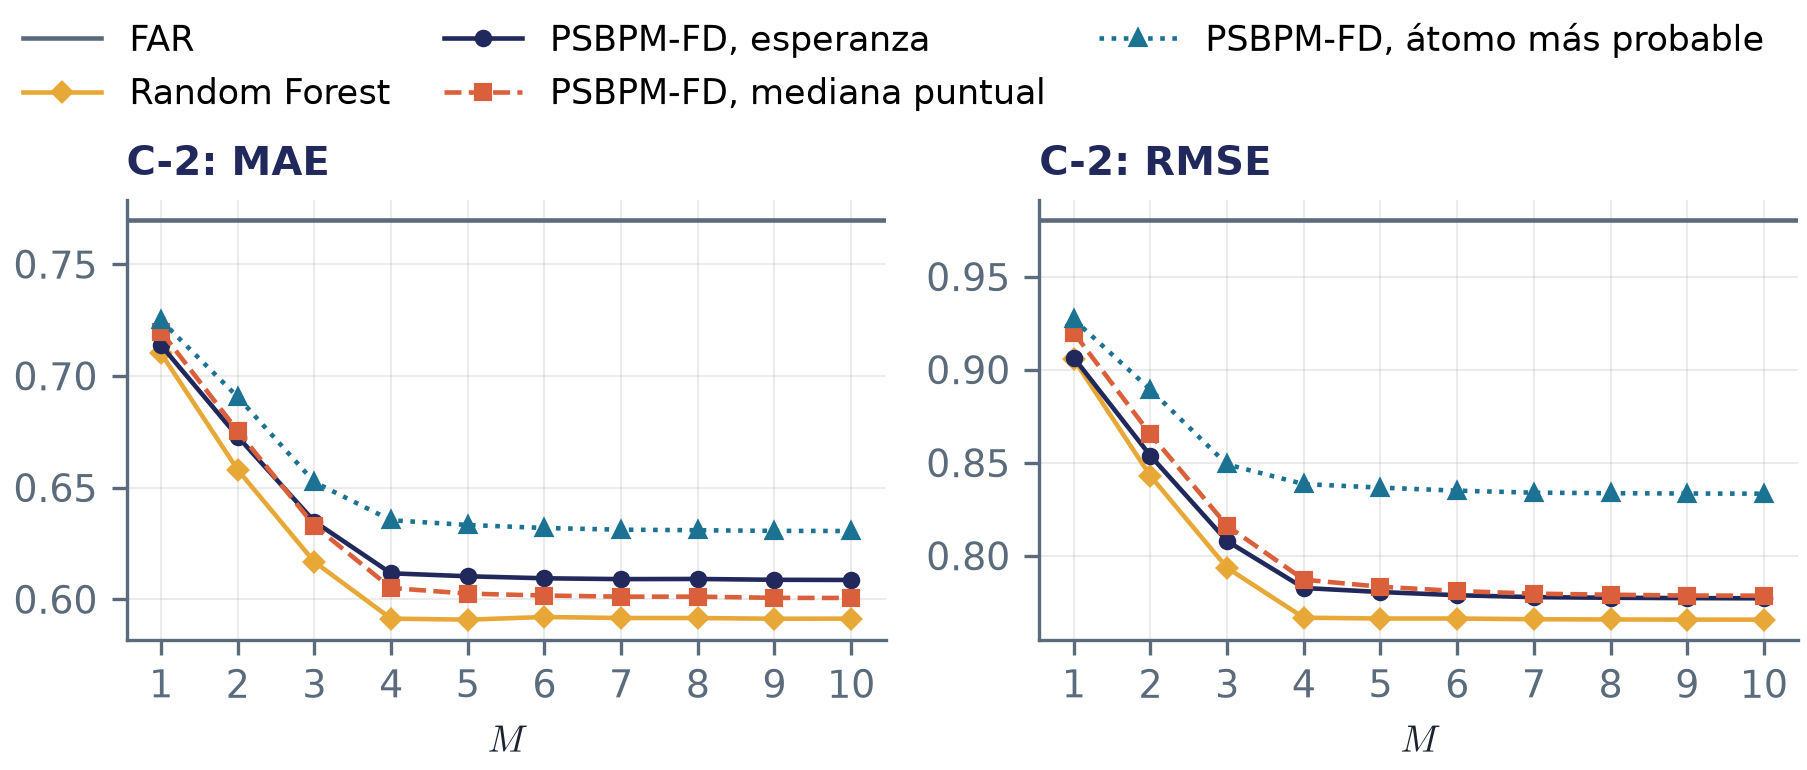
\includegraphics[width=\textwidth]{IMG/03_08/03_08_bloqueA_vs_M_C2.png}
\caption{C-2. MAE y RMSE en el bloque de prueba contra $M$.}
\label{fig:res_bloqueA_vs_M_C2}
\end{figure}

\begin{figure}[H]
\centering
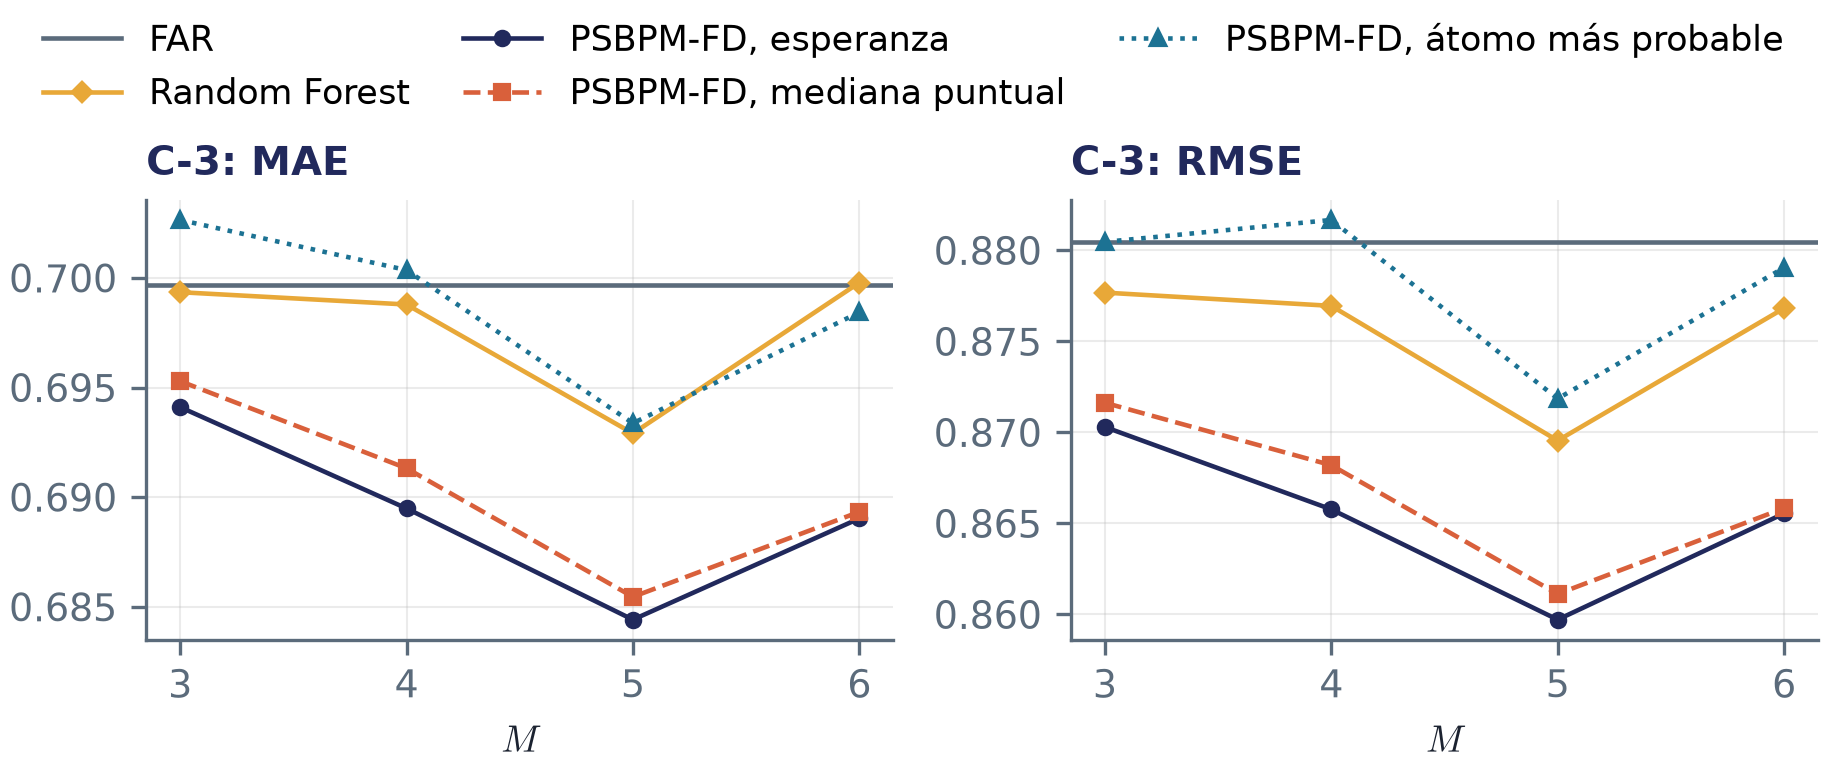
\includegraphics[width=\textwidth]{IMG/03_08/03_08_bloqueA_vs_M_C3.png}
\caption{C-3. MAE y RMSE en el bloque de prueba contra $M$.}
\label{fig:res_bloqueA_vs_M_C3}
\end{figure}
% Lectura M: el error decae hasta M = 4 (los J_a = 4 scores activos del generador) y después queda plano.
En las Figuras~\ref{fig:res_bloqueA_vs_M_C1} a~\ref{fig:res_bloqueA_vs_M_C3}, el error de todos los métodos que operan sobre los scores disminuye a medida que aumenta $M$, y lo hace de forma consistente en ambas métricas y en los tres escenarios. Se observa una caída pronunciada entre $M = 1$ y $M = 4$, seguida de un tramo plano en el que los valores solo varían en la tercera cifra. Esta caída se explica porque el error se mide contra la curva completa, por tanto la representación con $M$ scores omite la varianza de los $J - M$ restantes, y cada score adicional la recupera. El quiebre en $M = 4$ coincide con el diseño del generador. La dinámica de cada escenario reside en los $J_a = 4$ primeros scores, mientras que los seis restantes son autorregresivos débiles, casi impredecibles; incluirlos devuelve su varianza a la curva, pero no aporta información útil para la predicción. El FAR, que utiliza los $J$ coeficientes, sirve como referencia del truncamiento. Con $M \le 2$ gana en C-1 por construcción; la mezcla lo alcanza en $M = 3$ y lo supera desde $M = 4$. En C-2 lo supera ya con $M = 1$, porque el primer score concentra la mayor parte de la varianza y es el que más cambia de régimen. En C-3, donde las covariables son los rezagos de todos los scores y la dimensión del estado crece con $M$, el mínimo se alcanza en $M = 5$, mientras que $M = 6$ empeora, porque el sexto score es pasivo y lo que aporta como covariable a los pesos de la mezcla es ruido. El Random Forest sigue la misma trayectoria que el PSBPM-FD, ya que ve los mismos scores, y la distancia entre ambos se abre hasta $M = 4$ y después queda fija.

% Fuente: 98_resumen_bloqueA_min_max_prom.csv del _05 (test, M_ref); cambio relativo del promedio respecto del FAR.
\begin{table}[H]
\centering\footnotesize
\setlength{\tabcolsep}{4pt}
\caption{Cambio relativo del MAE y del RMSE respecto del FAR en $M_{\mathrm{ref}}$, por predictor y escenario. Negativo es mejor que el FAR.}
\label{tab:res_bloqueA_ganancia}
\begin{tabular}{l cc cc cc}
\hline
 & \multicolumn{2}{c}{C-1} & \multicolumn{2}{c}{C-2} & \multicolumn{2}{c}{C-3} \\
 & MAE & RMSE & MAE & RMSE & MAE & RMSE \\
\hline
PSBPM-FD, esperanza & $-1.7\%$ & $-1.7\%$ & $-20.9\%$ & $-20.7\%$ & $-1.5\%$ & $-1.7\%$ \\
PSBPM-FD, mediana puntual & $-1.6\%$ & $-1.6\%$ & $-22.0\%$ & $-20.6\%$ & $-1.5\%$ & $-1.7\%$ \\
PSBPM-FD, átomo más probable & $-0.9\%$ & $-0.6\%$ & $-18.1\%$ & $-15.0\%$ & $-0.2\%$ & $-0.2\%$ \\
Random Forest & $+1.5\%$ & $+1.6\%$ & $-23.2\%$ & $-21.9\%$ & $+0.0\%$ & $-0.4\%$ \\
\hline
\end{tabular}
\end{table}

% Lectura ganancia: el promedio dice cuánto se gana por estimador y en general.
El Cuadro~\ref{tab:res_bloqueA_ganancia} resume cuánto se gana en promedio respecto del FAR con cada estimador. En C-2 la ganancia es grande, en torno a un quinto del error en las dos métricas, y en C-1 y C-3 es pequeña, del orden del $2\%$. En los tres escenarios la esperanza y la mediana puntual ganan prácticamente lo mismo y el átomo más probable gana menos, porque se queda con un solo átomo por score y descarta la masa de los otros. La mediana puntual es el mejor estimador bajo MAE en C-2, donde la predictiva es bimodal en parte de los orígenes, y la esperanza lo es bajo RMSE en los tres escenarios, que es el reparto que corresponde a lo que cada métrica mide. El Random Forest, con las mismas covariables, gana más que el PSBPM-FD en C-2 y tiene un error mayor que el del FAR en C-1.

% Fuente: 72_ventana_modelos_w30.csv del _05 (test, M_ref, w = 30, sin el medoide); porcentaje de las 271 ventanas.
% Abajo: el predictor consistente con cada métrica (mediana puntual en C-2 y esperanza en C-1 y C-3 para el MAE; esperanza para el RMSE) contra cada referencia.
\begin{table}[H]
\centering\footnotesize
\caption{Ventanas de prueba ganadas en $M_{\mathrm{ref}}$. Arriba, fracción en que cada modelo es el mejor, abajo, fracción en que el predictor del PSBPM-FD supera a cada referencia.}
\label{tab:res_bloqueA_ventanas}
\begin{tabular}{l cc cc cc}
\hline
 & \multicolumn{2}{c}{C-1} & \multicolumn{2}{c}{C-2} & \multicolumn{2}{c}{C-3} \\
 & MAE & RMSE & MAE & RMSE & MAE & RMSE \\
\hline
FAR & 12\% & 7\% & 0\% & 0\% & 13\% & 7\% \\
Random Forest & 6\% & 3\% & 64\% & 60\% & 14\% & 15\% \\
PSBPM-FD, esperanza & 28\% & 56\% & 4\% & 21\% & 31\% & 36\% \\
PSBPM-FD, mediana puntual & 35\% & 25\% & 31\% & 19\% & 23\% & 30\% \\
PSBPM-FD, átomo más probable & 19\% & 9\% & 0\% & 0\% & 20\% & 11\% \\
\hline
PSBPM-FD gana al FAR & 87\% & 93\% & 100\% & 100\% & 85\% & 89\% \\
PSBPM-FD gana al Random Forest & 92\% & 96\% & 35\% & 31\% & 82\% & 83\% \\
\hline
\end{tabular}
\end{table}



% Lectura 2b: las ventanas. Una diferencia grande en el promedio se traduce en ganar casi todas las ventanas; una pequeña, en una mayoría.
Los promedios reflejan el comportamiento anteriormente descrito, porque los predictores puntuales del PSBPM-FD ganan la mayoría de las ventanas de prueba, cerca de nueve de cada diez frente al FAR y frente al Random Forest en C-1 y C-3, aunque ahí los promedios queden cerca, y todas las ventanas frente al FAR en C-2. La ventaja del Cuadro~\ref{tab:res_bloqueA_ganancia} no viene de un tramo particular del bloque de prueba sino que se repite a lo largo de él. Entre los predictores del PSBPM-FD el reparto sigue a la métrica, con la mediana puntual ganando más ventanas bajo MAE y la esperanza bajo RMSE, y el Random Forest gana dos de cada tres ventanas en C-2 por lo mismo que gana el promedio.


\begin{figure}[H]
\centering
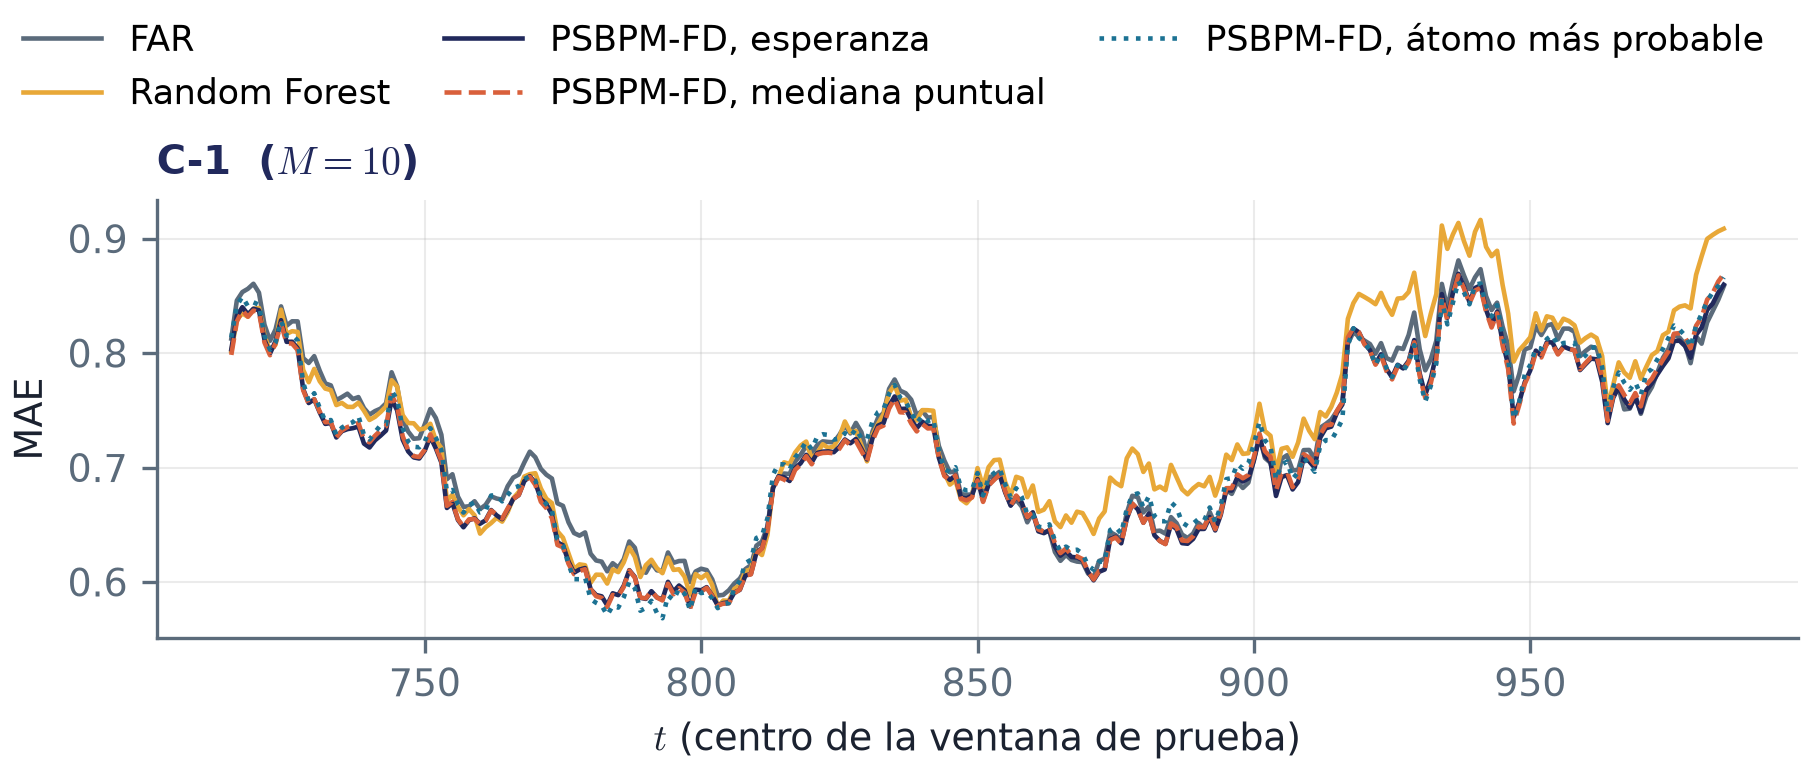
\includegraphics[width=\textwidth]{IMG/03_08/03_08_bloqueA_ventana_w30_C1.png}
\caption{C-1. MAE sobre la ventana móvil del bloque de prueba ($M_{\mathrm{ref}}$).}
\label{fig:res_bloqueA_ventana_C1}
\end{figure}

\begin{figure}[H]
\centering
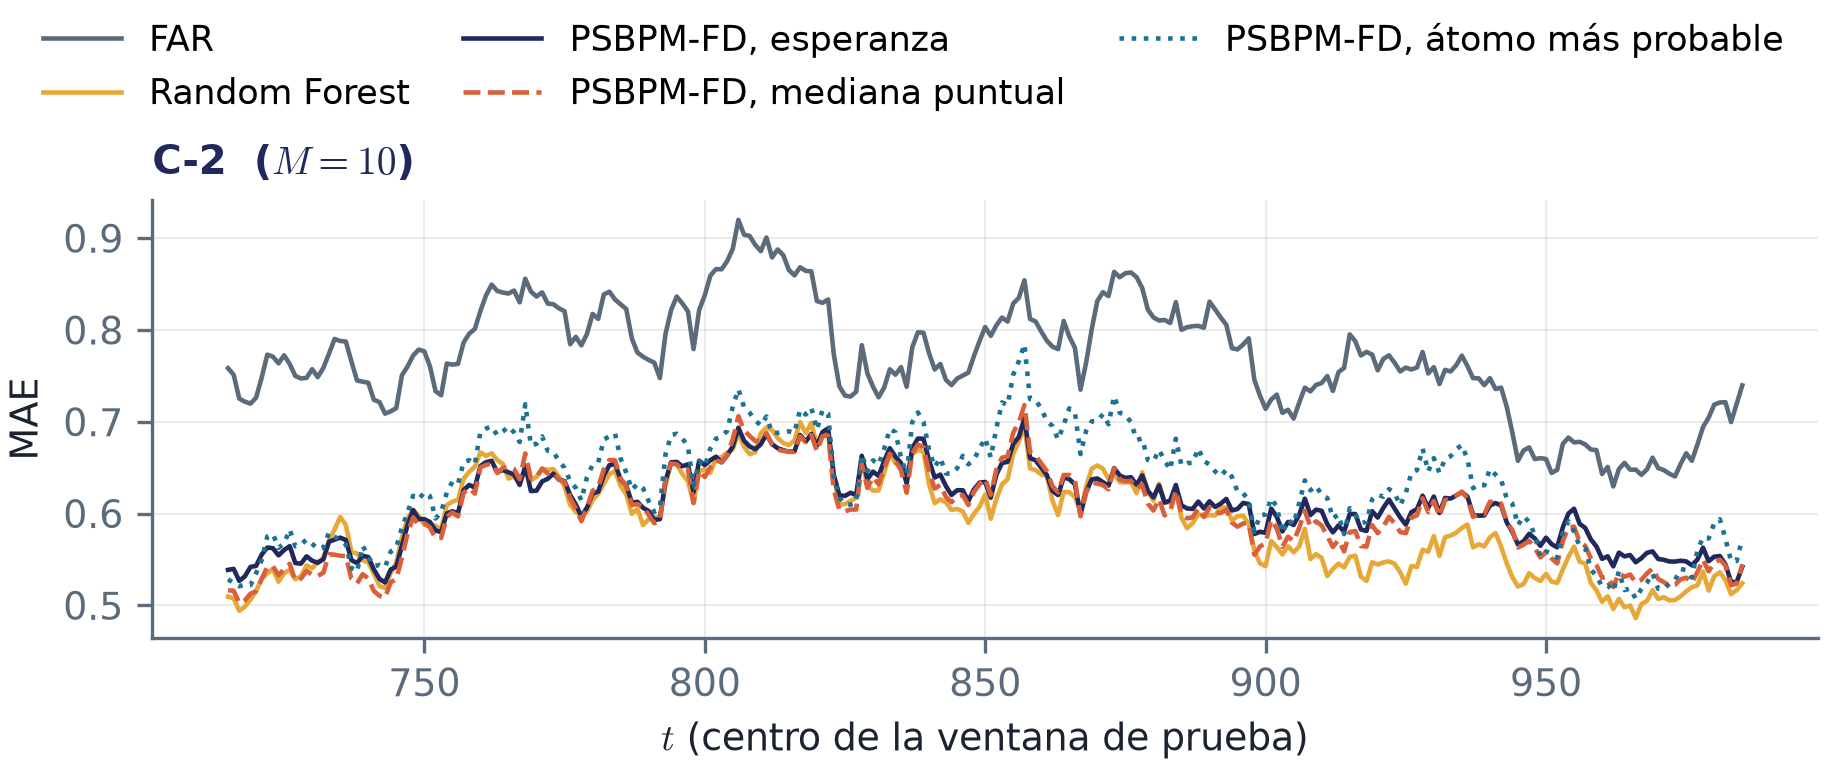
\includegraphics[width=\textwidth]{IMG/03_08/03_08_bloqueA_ventana_w30_C2.png}
\caption{C-2. MAE sobre la ventana móvil del bloque de prueba ($M_{\mathrm{ref}}$).}
\label{fig:res_bloqueA_ventana_C2}
\end{figure}

\begin{figure}[H]
\centering
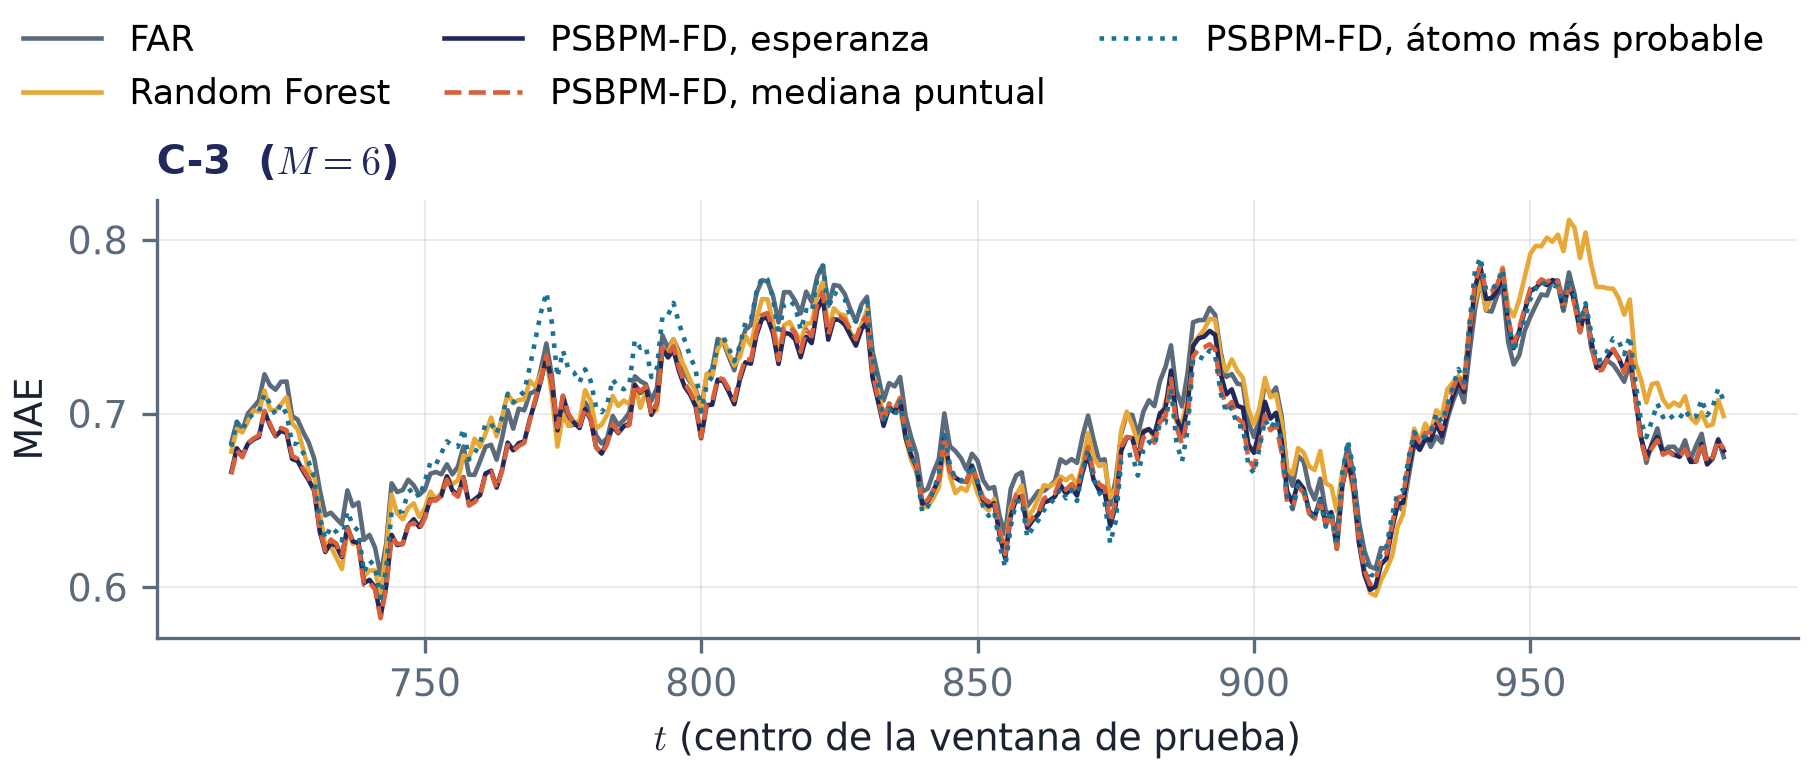
\includegraphics[width=\textwidth]{IMG/03_08/03_08_bloqueA_ventana_w30_C3.png}
\caption{C-3. MAE sobre la ventana móvil del bloque de prueba ($M_{\mathrm{ref}}$).}
\label{fig:res_bloqueA_ventana_C3}
\end{figure}
% Lectura 4: dónde gana a lo largo del test (tramos, no promedio).
Las Figuras~\ref{fig:res_bloqueA_ventana_C1} a~\ref{fig:res_bloqueA_ventana_C3} muestran que en C-2 la brecha con el FAR es uniforme, porque los regímenes cambian cada pocas curvas y toda ventana contiene ambos. En C-1 y C-3 todos los modelos suben y bajan juntos, porque el error está dominado por la innovación, que ningún modelo predice, y en C-1 su varianza cambia con el tiempo. Lo que distingue a los modelos es pequeño frente a eso, y se ve solo en los tramos tranquilos, donde el FAR queda por encima, y en el tramo final de C-1 y C-3, donde el Random Forest se despega hacia arriba.

\subsection{Intervalos de predicción}
\label{03_08_02_intervalos}

Los Cuadros~\ref{tab:res_bloqueB_por_M} a~\ref{tab:res_bloqueB_picp_por_M} resumen el Winkler, el MPIW y el PICP promedio sobre las ventanas de prueba, contra la curva ajustada, de las tres construcciones de intervalo del PSBPM-FD y de la banda gaussiana del FAR, para cada $M$ del barrido. Las Figuras~\ref{fig:res_bloqueB_vs_M_C1} a~\ref{fig:res_bloqueB_vs_M_C3} muestran las mismas cifras contra $M$, el Cuadro~\ref{tab:res_bloqueB_ganancia} cuánto cambia cada métrica respecto del FAR en $M_{\mathrm{ref}}$ y el Cuadro~\ref{tab:res_bloqueB_ventanas} cómo se reparten las ventanas entre las bandas.

% Fuente: 99_resumen_bloqueB_min_max_prom.csv del _05 (test, promedio sobre las ventanas, todas las bandas y M).
\begin{table}[H]
\centering\footnotesize
\setlength{\tabcolsep}{4pt}
\caption{Winkler en el bloque de prueba por escenario y $M$. En negrita el menor entre las construcciones en $M_{\mathrm{ref}}$, menor es mejor.}
\label{tab:res_bloqueB_por_M}
\begin{tabular}{c ccc ccc ccc}
\hline
 & \multicolumn{3}{c}{C-1} & \multicolumn{3}{c}{C-2} & \multicolumn{3}{c}{C-3} \\
$M$ & Equi-colas & HDR & Simult. & Equi-colas & HDR & Simult. & Equi-colas & HDR & Simult. \\
\hline
$1$ & 9.94 & 9.93 & 9.92 & 11.95 & 12.09 & 10.74 & --- & --- & --- \\
$2$ & 4.98 & 4.94 & 4.44 & 5.69 & 5.29 & 6.54 & --- & --- & --- \\
$3$ & 4.49 & 4.46 & 4.68 & 4.61 & 4.31 & 7.91 & 4.31 & 4.31 & 4.42 \\
$4$ & 4.32 & 4.30 & 4.92 & 3.97 & 3.75 & 6.73 & 4.15 & 4.16 & 4.71 \\
$5$ & 4.27 & 4.26 & 5.11 & 3.91 & 3.75 & 6.57 & 4.08 & 4.09 & 4.89 \\
$6$ & 4.24 & 4.24 & 5.19 & 3.90 & 3.76 & 6.32 & \textbf{4.11} & \textbf{4.11} & 4.99 \\
$7$ & 4.23 & 4.23 & 5.26 & 3.90 & 3.77 & 6.41 & --- & --- & --- \\
$8$ & 4.23 & 4.23 & 5.29 & 3.91 & 3.78 & 6.36 & --- & --- & --- \\
$9$ & 4.23 & 4.23 & 5.32 & 3.91 & 3.79 & 6.37 & --- & --- & --- \\
$10$ & \textbf{4.23} & \textbf{4.23} & 5.33 & 3.91 & \textbf{3.79} & 6.36 & --- & --- & --- \\
\hline
FAR & \multicolumn{3}{c}{4.35} & \multicolumn{3}{c}{4.86} & \multicolumn{3}{c}{4.23} \\
\hline
\end{tabular}
\end{table}

\begin{table}[H]
\centering\footnotesize
\setlength{\tabcolsep}{4pt}
\caption{MPIW en el bloque de prueba por escenario y $M$.}
\label{tab:res_bloqueB_mpiw_por_M}
\begin{tabular}{c ccc ccc ccc}
\hline
 & \multicolumn{3}{c}{C-1} & \multicolumn{3}{c}{C-2} & \multicolumn{3}{c}{C-3} \\
$M$ & Equi-colas & HDR & Simult. & Equi-colas & HDR & Simult. & Equi-colas & HDR & Simult. \\
\hline
$1$ & 1.95 & 1.95 & 1.96 & 1.76 & 1.46 & 2.01 & --- & --- & --- \\
$2$ & 2.82 & 2.82 & 3.70 & 2.79 & 2.56 & 6.08 & --- & --- & --- \\
$3$ & 3.09 & 3.10 & 4.39 & 3.14 & 2.97 & 7.79 & 2.98 & 2.98 & 4.16 \\
$4$ & 3.26 & 3.27 & 4.78 & 3.35 & 3.23 & 6.71 & 3.16 & 3.17 & 4.59 \\
$5$ & 3.37 & 3.37 & 5.01 & 3.45 & 3.35 & 6.55 & 3.26 & 3.27 & 4.80 \\
$6$ & 3.43 & 3.43 & 5.12 & 3.51 & 3.42 & 6.31 & 3.33 & 3.33 & 4.93 \\
$7$ & 3.45 & 3.46 & 5.19 & 3.54 & 3.45 & 6.40 & --- & --- & --- \\
$8$ & 3.47 & 3.48 & 5.23 & 3.56 & 3.47 & 6.34 & --- & --- & --- \\
$9$ & 3.48 & 3.49 & 5.25 & 3.57 & 3.49 & 6.35 & --- & --- & --- \\
$10$ & 3.49 & 3.49 & 5.26 & 3.58 & 3.49 & 6.35 & --- & --- & --- \\
\hline
FAR & \multicolumn{3}{c}{3.42} & \multicolumn{3}{c}{3.98} & \multicolumn{3}{c}{3.28} \\
\hline
\end{tabular}
\end{table}

\begin{table}[H]
\centering\footnotesize
\setlength{\tabcolsep}{4pt}
\caption{PICP en el bloque de prueba por escenario y $M$.}
\label{tab:res_bloqueB_picp_por_M}
\begin{tabular}{c ccc ccc ccc}
\hline
 & \multicolumn{3}{c}{C-1} & \multicolumn{3}{c}{C-2} & \multicolumn{3}{c}{C-3} \\
$M$ & Equi-colas & HDR & Simult. & Equi-colas & HDR & Simult. & Equi-colas & HDR & Simult. \\
\hline
$1$ & 0.640 & 0.640 & 0.641 & 0.541 & 0.493 & 0.604 & --- & --- & --- \\
$2$ & 0.869 & 0.872 & 0.953 & 0.817 & 0.813 & 0.968 & --- & --- & --- \\
$3$ & 0.910 & 0.911 & 0.979 & 0.891 & 0.899 & 0.992 & 0.908 & 0.910 & 0.980 \\
$4$ & 0.932 & 0.932 & 0.990 & 0.945 & 0.955 & 0.998 & 0.931 & 0.931 & 0.991 \\
$5$ & 0.939 & 0.942 & 0.993 & 0.957 & 0.965 & 0.999 & 0.943 & 0.942 & 0.993 \\
$6$ & 0.943 & 0.945 & 0.994 & 0.964 & 0.971 & 0.999 & 0.944 & 0.945 & 0.995 \\
$7$ & 0.945 & 0.947 & 0.995 & 0.967 & 0.974 & 0.999 & --- & --- & --- \\
$8$ & 0.946 & 0.948 & 0.995 & 0.968 & 0.974 & 0.999 & --- & --- & --- \\
$9$ & 0.946 & 0.948 & 0.995 & 0.968 & 0.975 & 0.999 & --- & --- & --- \\
$10$ & 0.947 & 0.948 & 0.995 & 0.969 & 0.975 & 0.999 & --- & --- & --- \\
\hline
FAR & \multicolumn{3}{c}{0.940} & \multicolumn{3}{c}{0.952} & \multicolumn{3}{c}{0.937} \\
\hline
\end{tabular}
\end{table}

% Figura Bloque B contra M: Winkler, MPIW y PICP de las tres construcciones y del FAR. Fuente: 99_* del _05.
\begin{figure}[H]
\centering
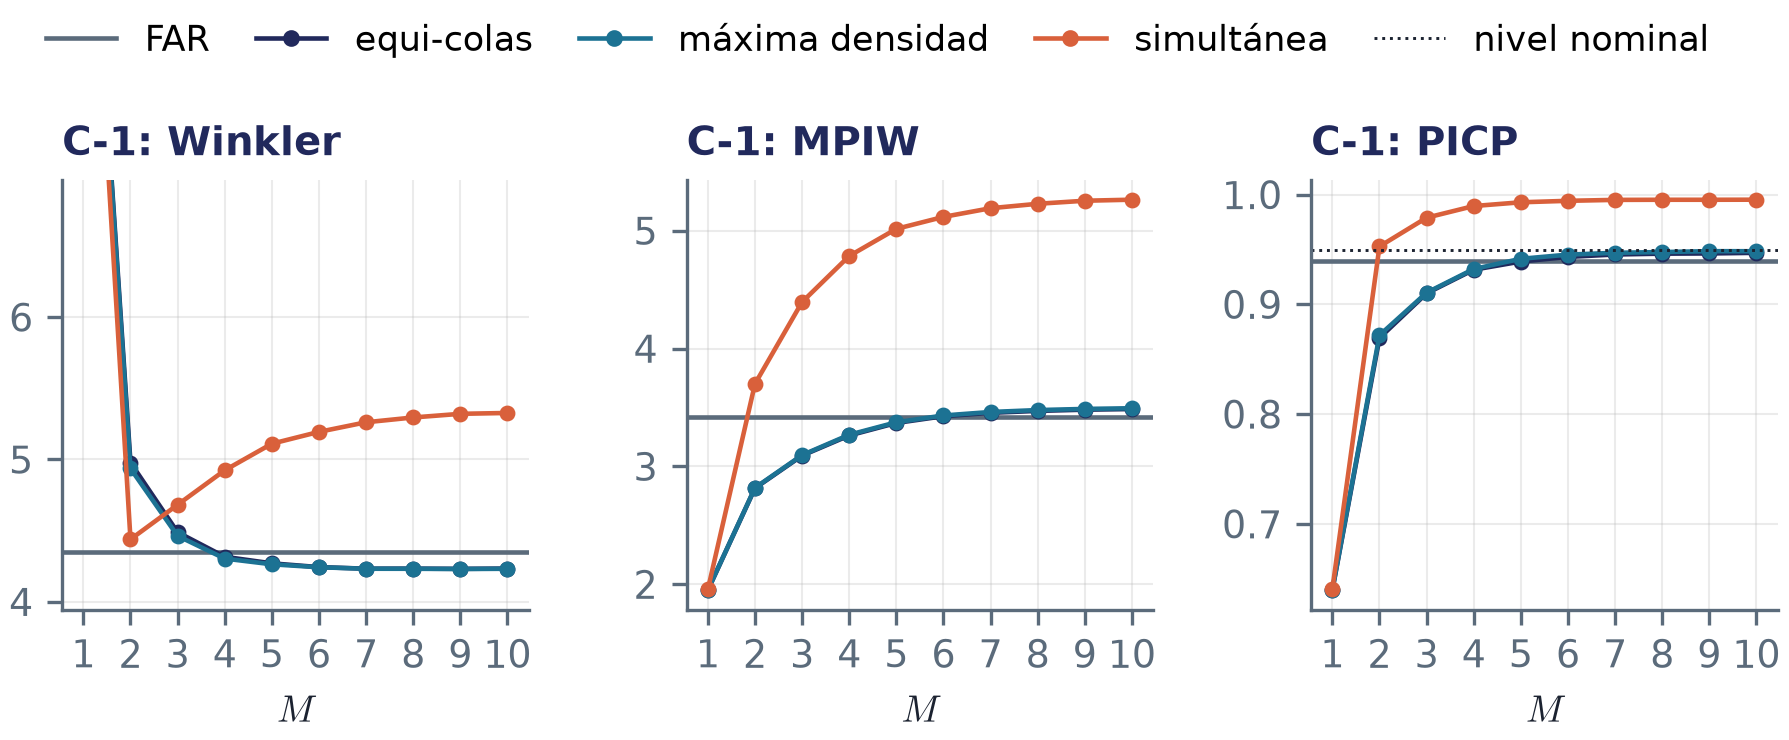
\includegraphics[width=\textwidth]{IMG/03_08/03_08_bloqueB_vs_M_C1.png}
\caption{C-1. Winkler, MPIW y PICP en el bloque de prueba contra $M$. El eje del Winkler se corta para que $M = 1$ no aplaste el resto.}
\label{fig:res_bloqueB_vs_M_C1}
\end{figure}

\begin{figure}[H]
\centering
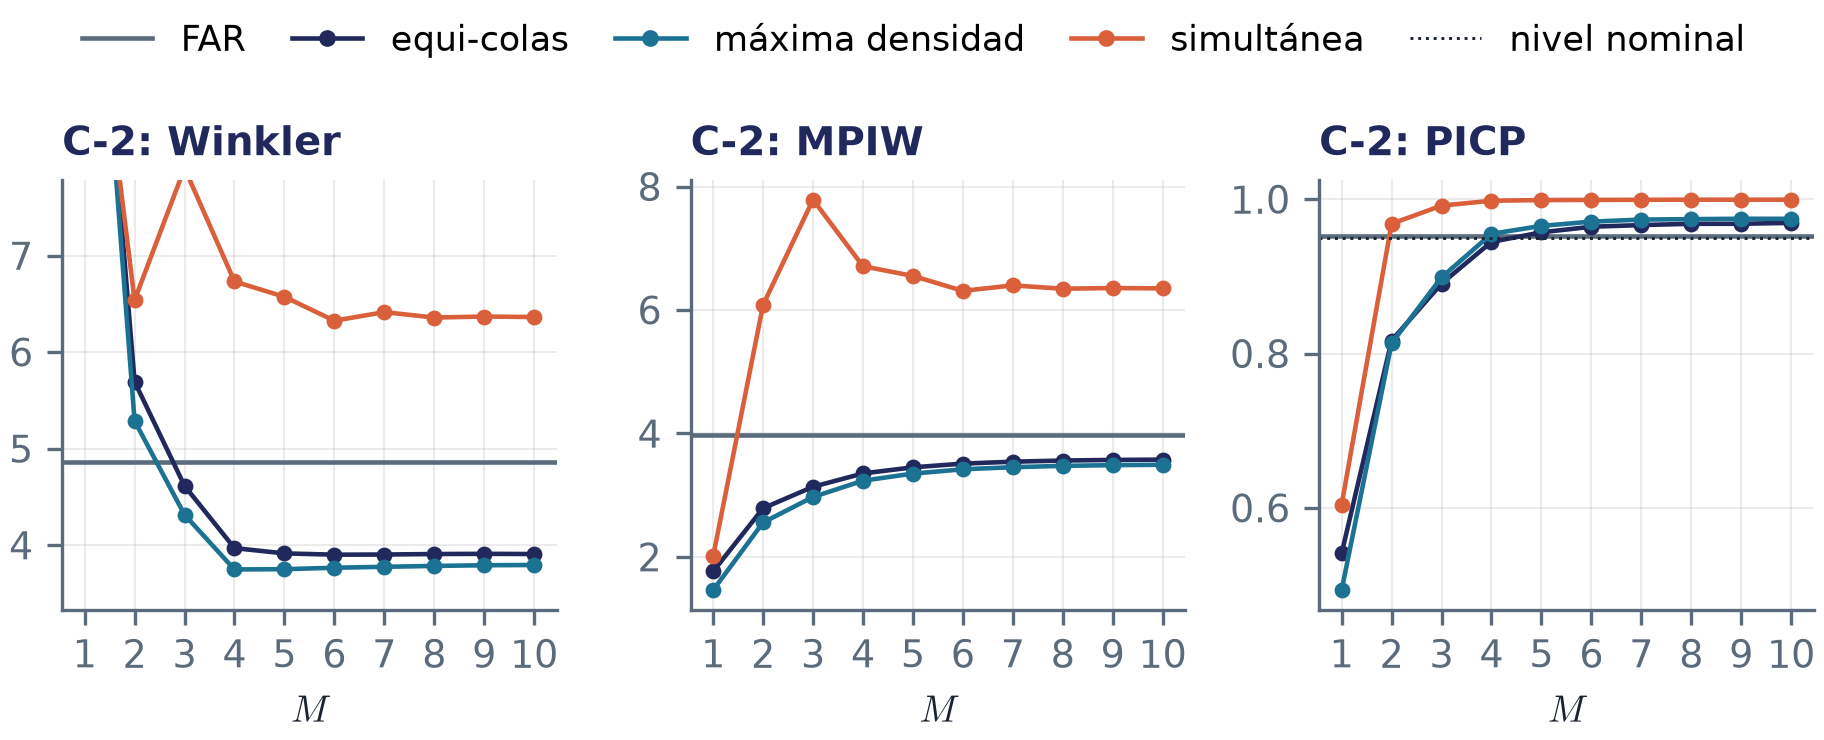
\includegraphics[width=\textwidth]{IMG/03_08/03_08_bloqueB_vs_M_C2.png}
\caption{C-2. Winkler, MPIW y PICP en el bloque de prueba contra $M$. El eje del Winkler se corta para que $M = 1$ no aplaste el resto.}
\label{fig:res_bloqueB_vs_M_C2}
\end{figure}

\begin{figure}[H]
\centering
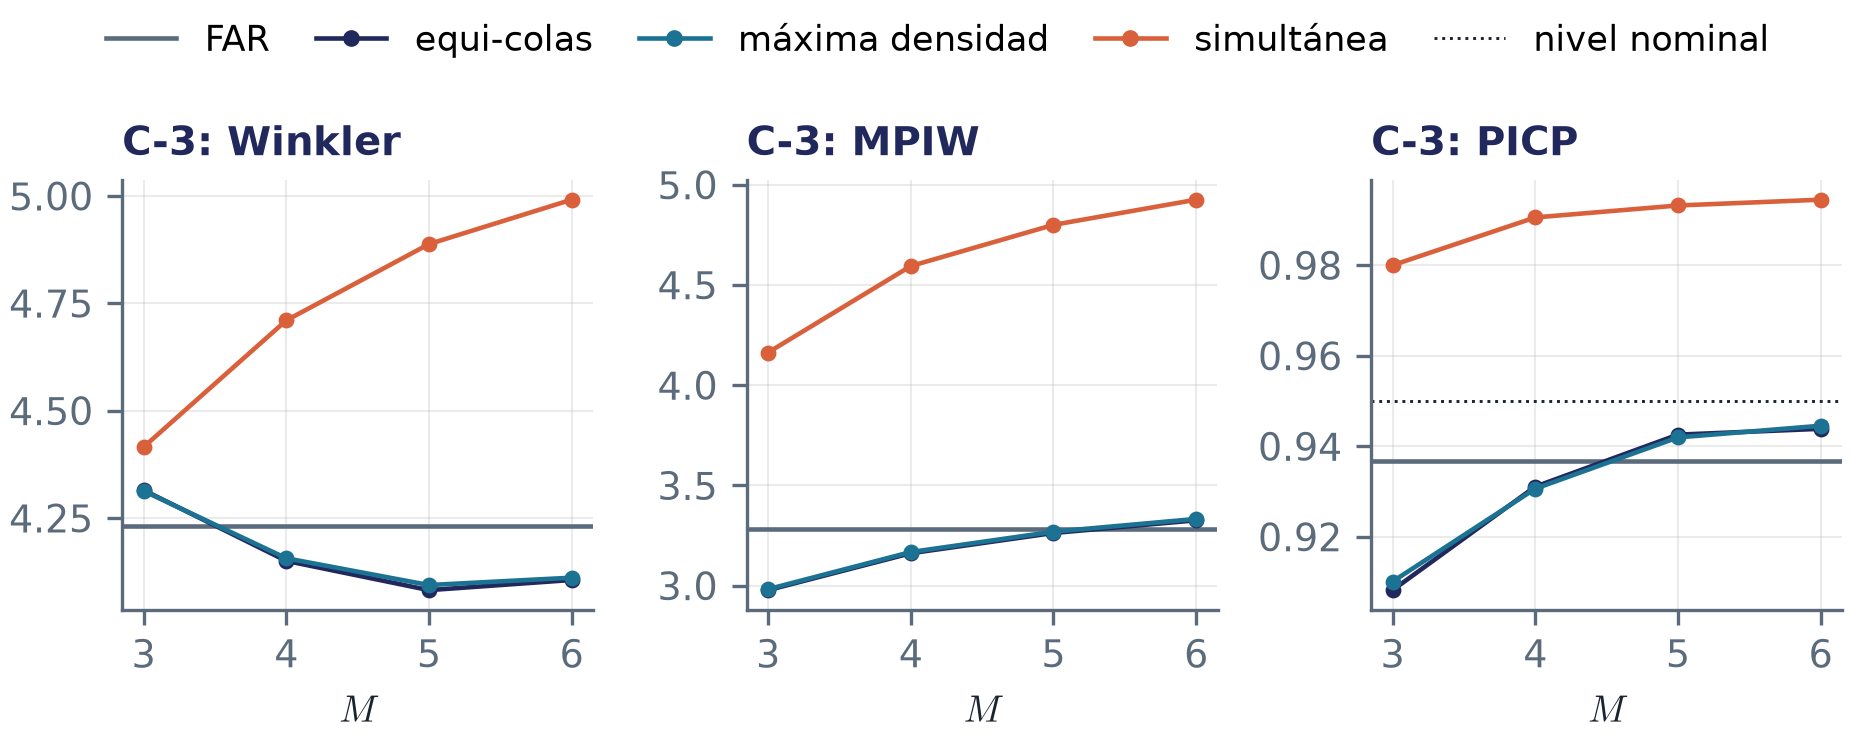
\includegraphics[width=\textwidth]{IMG/03_08/03_08_bloqueB_vs_M_C3.png}
\caption{C-3. Winkler, MPIW y PICP en el bloque de prueba contra $M$. El eje del Winkler se corta para que $M = 1$ no aplaste el resto.}
\label{fig:res_bloqueB_vs_M_C3}
\end{figure}

% Lectura M: las bandas mejoran hasta M = 4 por la misma razón que el error puntual, y la simultánea es la única que sigue ensanchándose.
En las Figuras~\ref{fig:res_bloqueB_vs_M_C1} a~\ref{fig:res_bloqueB_vs_M_C3} las tres métricas se mueven con $M$ de la misma forma en los tres escenarios. Con $M = 1$ la banda cubre solo la variabilidad del primer score y deja fuera la de los demás, que sí están en la curva contra la que se mide, por eso es angosta, su PICP queda muy por debajo del nominal y su Winkler es más del doble del FAR. Cada score que entra agrega su dispersión a la banda, el MPIW crece, el PICP sube hacia el nominal y el Winkler baja, y desde $M = 4$ las tres quedan planas, igual que el error puntual y por la misma razón, porque los seis scores restantes son pasivos. Las bandas puntuales, equi-colas y máxima densidad, se estabilizan en un PICP cercano al nominal con un ancho parecido al del FAR. En C-1 y C-3 la simultánea es la única que sigue ensanchándose con $M$, porque debe contener la curva entera y el supremo sobre el dominio crece con cada score que se agrega aunque este aporte poco a cada punto; en C-2 su ancho baja desde $M = 3$. Solo es la mejor de las tres con $M \le 2$ en C-1 y con $M = 1$ en C-2, cuando las otras dos todavía quedan cortas.

% Fuente: 99_resumen_bloqueB_min_max_prom.csv del _05 (test, M_ref); cambio relativo del promedio respecto del FAR.
\begin{table}[H]
\centering\small
\caption{Cambio relativo del Winkler, el MPIW y el PICP respecto del FAR en $M_{\mathrm{ref}}$, por escenario y construcción. En el Winkler y el MPIW negativo es mejor que el FAR, en el PICP positivo es más cobertura.}
\label{tab:res_bloqueB_ganancia}
\begin{tabular}{l l ccc}
\hline
Escenario & Banda & Winkler & MPIW & PICP \\
\hline
C-1 & Equi-colas & $-2.7\%$ & $+1.9\%$ & $+0.7\%$ \\
 & Máxima densidad & $-2.8\%$ & $+2.1\%$ & $+0.9\%$ \\
 & Simultánea & $+22.4\%$ & $+53.7\%$ & $+5.9\%$ \\
\hline
C-2 & Equi-colas & $-19.7\%$ & $-10.1\%$ & $+1.8\%$ \\
 & Máxima densidad & $-22.0\%$ & $-12.2\%$ & $+2.4\%$ \\
 & Simultánea & $+30.8\%$ & $+59.7\%$ & $+5.0\%$ \\
\hline
C-3 & Equi-colas & $-3.0\%$ & $+1.3\%$ & $+0.8\%$ \\
 & Máxima densidad & $-2.8\%$ & $+1.5\%$ & $+0.8\%$ \\
 & Simultánea & $+18.0\%$ & $+50.0\%$ & $+6.2\%$ \\
\hline
\end{tabular}
\end{table}

% Lectura ganancia: cuánto se gana por construcción y de dónde viene (ancho o cobertura).
El Cuadro~\ref{tab:res_bloqueB_ganancia} dice cuánto se gana respecto del FAR con cada construcción y de dónde viene la ganancia, porque el Winkler suma el ancho y una penalización por los puntos no cubiertos. En C-2 las bandas puntuales bajan el Winkler en un quinto y lo hacen por las dos vías a la vez, una banda un $10\%$ más angosta que además cubre más. Eso solo es posible porque el ancho de la banda del PSBPM-FD sigue el régimen en que está cada score, mientras que el del FAR hereda una varianza residual fija y es el mismo en todos los orígenes. En C-1 y C-3 la ganancia es del orden del $3\%$ y tiene otra composición, la banda del PSBPM-FD es apenas más ancha y su PICP queda más cerca del nominal, de modo que gana por calibración y no por ancho. Esa ganancia pequeña se explica igual que en el error puntual, la referencia gaussiana está casi bien especificada cuando la media es lineal y la varianza cambia poco. La máxima densidad coincide con la equi-colas en C-1 y C-3, porque con una predictiva unimodal y simétrica ambas son el mismo intervalo central, y solo en C-2 la mejora, reasignando a los modos la masa que la equi-colas gasta en el valle entre ellos. La simultánea pierde el Winkler en los tres escenarios porque es entre $1.5$ y $1.6$ veces más ancha, que es lo que cuesta contener la curva entera y no cada punto por separado, y es la única construcción calibrada para esa cobertura. Queda por ver si estos promedios reflejan el comportamiento a lo largo del bloque de prueba.

% Fuente: 81_ventana_bloqueB_w30.csv del _05 (test, M_ref, w = 30); porcentaje de las 271 ventanas, por Winkler.
\begin{table}[H]
\centering\small
\caption{Ventanas de prueba ganadas en $M_{\mathrm{ref}}$ por Winkler. Arriba, fracción en que cada banda es la mejor, abajo, fracción en que cada construcción del PSBPM-FD supera al FAR.}
\label{tab:res_bloqueB_ventanas}
\begin{tabular}{l ccc}
\hline
 & C-1 & C-2 & C-3 \\
\hline
FAR & 11\% & 0\% & 18\% \\
Equi-colas & 35\% & 9\% & 46\% \\
Máxima densidad & 54\% & 91\% & 36\% \\
Simultánea & 0\% & 0\% & 0\% \\
\hline
Equi-colas gana al FAR & 81\% & 100\% & 81\% \\
Máxima densidad gana al FAR & 88\% & 100\% & 73\% \\
Simultánea gana al FAR & 5\% & 0\% & 1\% \\
\hline
\end{tabular}
\end{table}

% Lectura ventanas: los promedios reflejan el comportamiento.
 Las bandas puntuales del PSBPM-FD ganan al FAR en todas las ventanas de C-2 y en cuatro de cada cinco de C-1 y C-3, aunque ahí los promedios queden a un $3\%$, de modo que la ventaja se repite a lo largo del bloque de prueba y no viene de unos pocos tramos. Entre las construcciones, la máxima densidad es la mejor en nueve de cada diez ventanas de C-2, donde la predictiva tiene valles, y en C-1 y C-3 se reparte con la equi-colas porque son casi la misma banda. La simultánea no gana ninguna ventana por Winkler, que es lo esperable de una banda que ensancha el intervalo.

% Figura: Winkler sobre la ventana móvil de prueba, w_ref, M_ref. Fuente: 81_ventana_bloqueB_w30.csv del _05.
\begin{figure}[H]
\centering
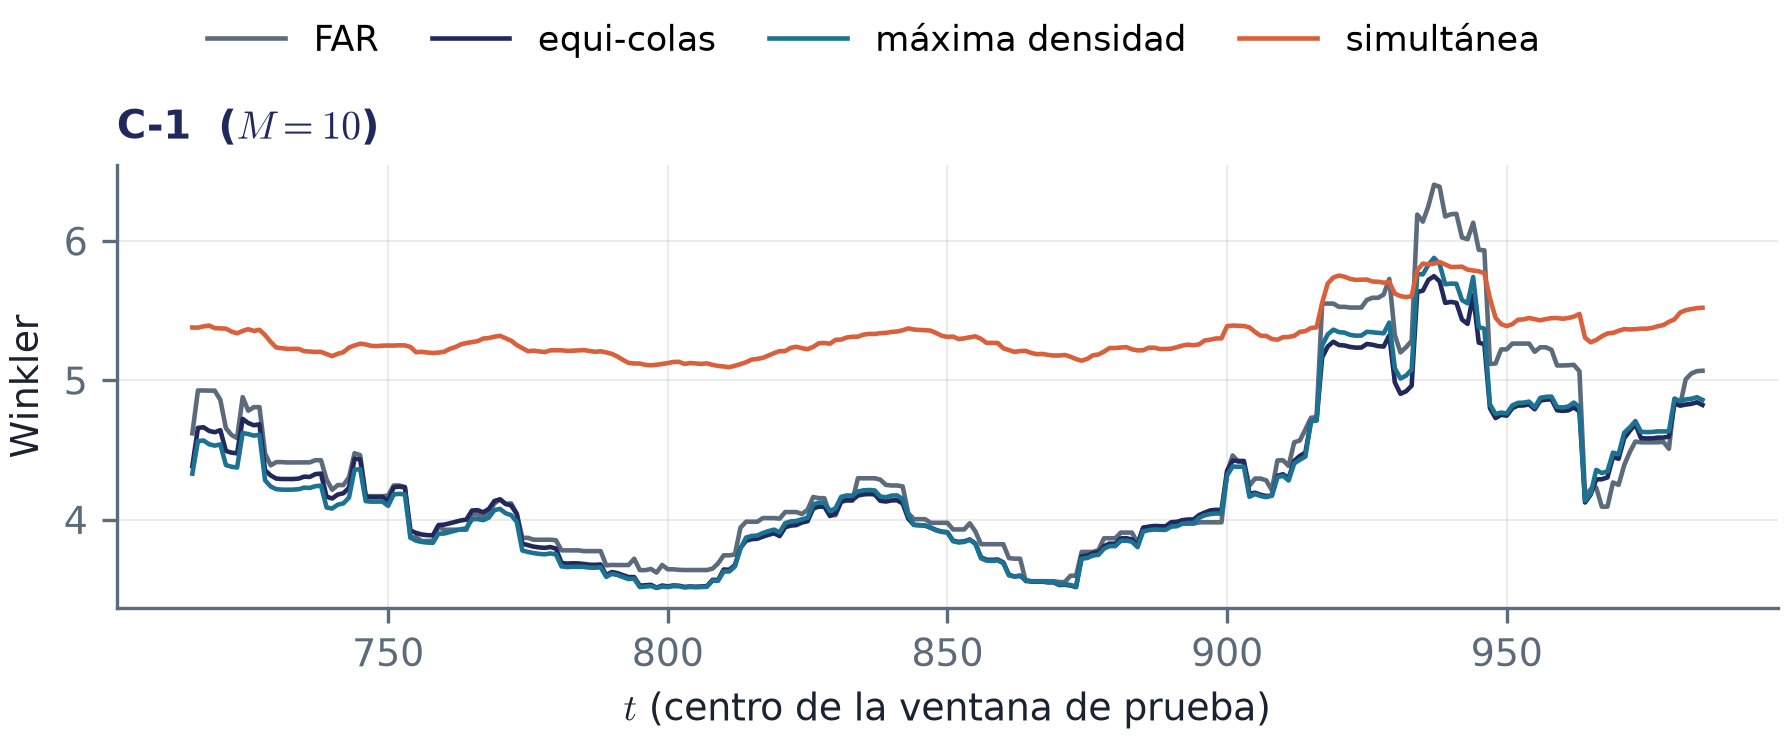
\includegraphics[width=\textwidth]{IMG/03_08/03_08_bloqueB_ventana_w30_C1.png}
\caption{C-1. Winkler sobre la ventana móvil del bloque de prueba ($M_{\mathrm{ref}}$).}
\label{fig:res_bloqueB_ventana_C1}
\end{figure}

\begin{figure}[H]
\centering
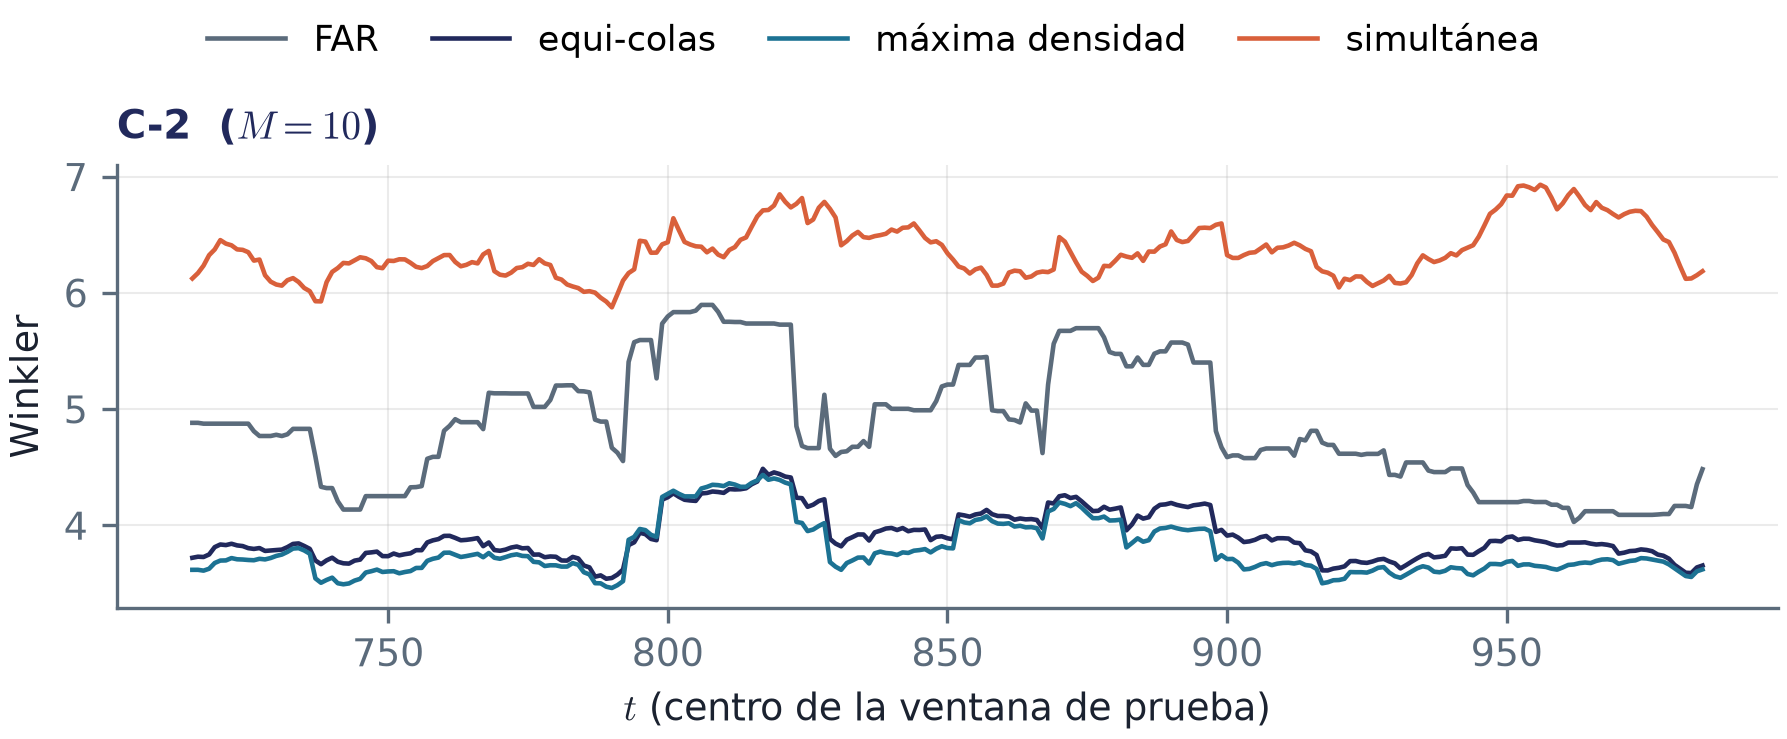
\includegraphics[width=\textwidth]{IMG/03_08/03_08_bloqueB_ventana_w30_C2.png}
\caption{C-2. Winkler sobre la ventana móvil del bloque de prueba ($M_{\mathrm{ref}}$).}
\label{fig:res_bloqueB_ventana_C2}
\end{figure}

\begin{figure}[H]
\centering
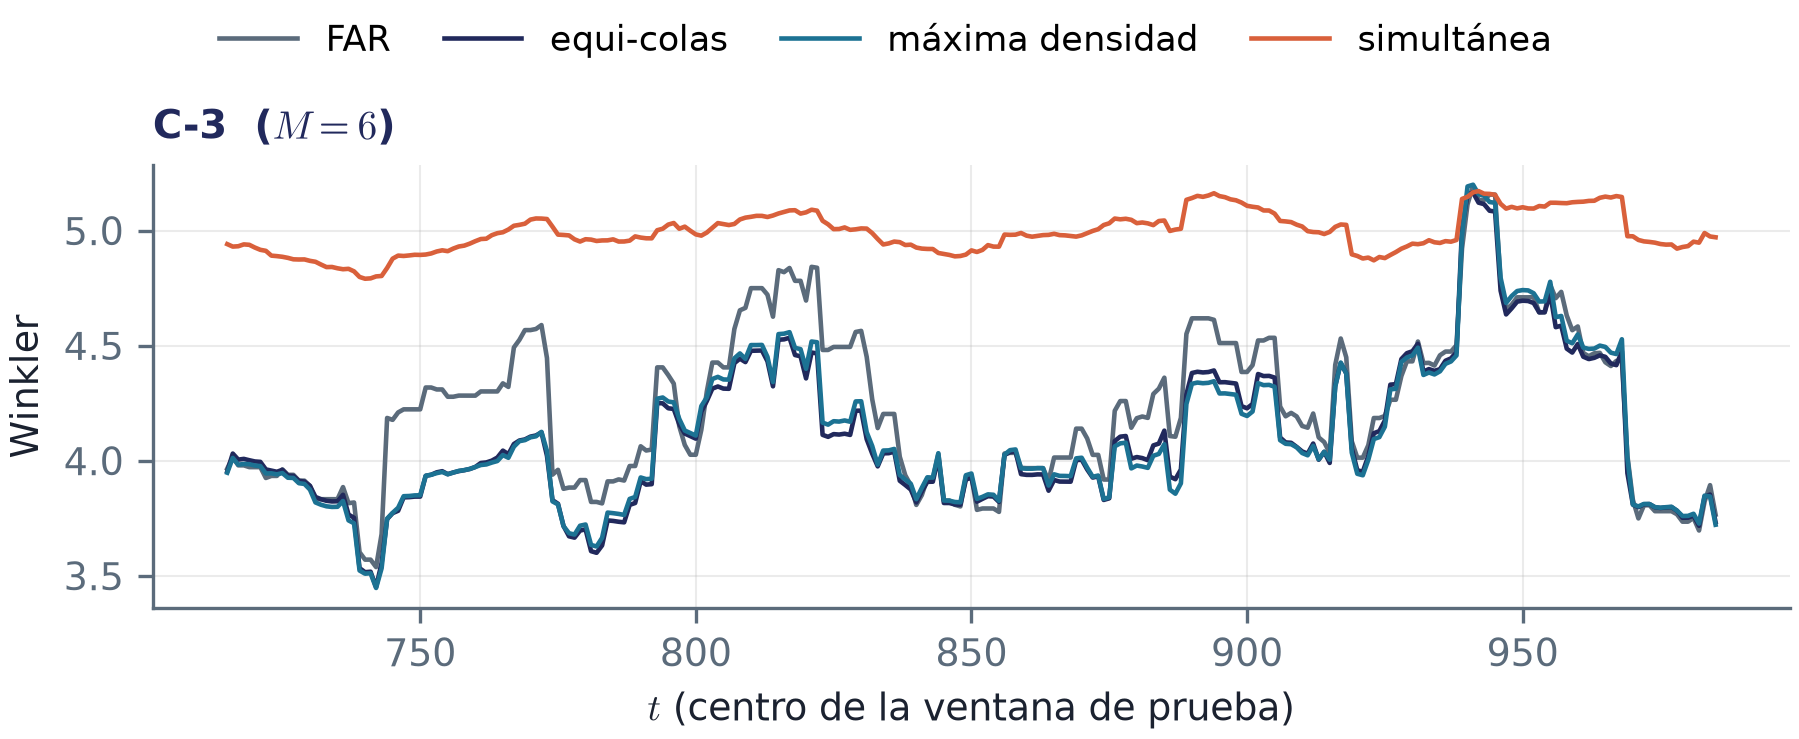
\includegraphics[width=\textwidth]{IMG/03_08/03_08_bloqueB_ventana_w30_C3.png}
\caption{C-3. Winkler sobre la ventana móvil del bloque de prueba ($M_{\mathrm{ref}}$).}
\label{fig:res_bloqueB_ventana_C3}
\end{figure}

% Lectura trayectoria: el ancho del FAR no depende del origen y el del PSBPM-FD sí. Ésa es la diferencia clave.
Las Figuras~\ref{fig:res_bloqueB_ventana_C1} a~\ref{fig:res_bloqueB_ventana_C3} muestran de dónde sale la diferencia. Con una cantidad suficiente de componentes para contener la dinámica, el PSBPM-FD adapta el ancho de su banda al estado del proceso en cada origen, mientras que la banda del FAR tiene el mismo ancho en todos los orígenes y su Winkler solo se mueve por la penalización de los puntos que deja fuera. Por eso en C-2 el Winkler del FAR sube cada vez que la ventana contiene episodios del régimen volátil y el del PSBPM-FD se mantiene estable y por debajo en todas las ventanas, porque la banda se ensancha en esos episodios y se angosta en los tranquilos. En C-1 las curvas suben juntas en el episodio de volatilidad del tramo final, alrededor de $t = 930$, donde la banda del PSBPM-FD se ensancha y acompaña al proceso, y la ventaja aparece en los tramos tranquilos, donde la banda gaussiana es más ancha de lo necesario. En C-3 las curvas se superponen y el FAR se despega hacia arriba en las ventanas con los peores errores. El modelo no es conservador por regla, es angosto donde el proceso está tranquilo y ancho donde cambia de régimen, y esa es la diferencia que una banda de ancho fijo no puede dar. Las Figuras~\ref{fig:res_bloqueB_ancho_C1} a~\ref{fig:res_bloqueB_ancho_C3} lo muestran de forma directa con el ancho medio de la banda en cada origen de prueba. El del FAR es una línea horizontal y el del PSBPM-FD se mueve con el estado del proceso, por debajo del FAR en los tramos tranquilos y por encima en los episodios en que la varianza condicional sube, en C-1, o en que algún score está en el régimen volátil, en C-2. En C-3 el ancho también cambia de origen en origen, aunque con menos amplitud, porque la dispersión de la mezcla depende de los rezagos aun cuando la media condicional sea casi lineal.

% Figura: ancho medio de la banda por origen de prueba. Fuente: banda_funcional_psbp.npz del _04 (li, ls, hdr_L, hdr_U, li/ls_simultanea) y el MPIW del FAR de 81_*.
\begin{figure}[H]
\centering
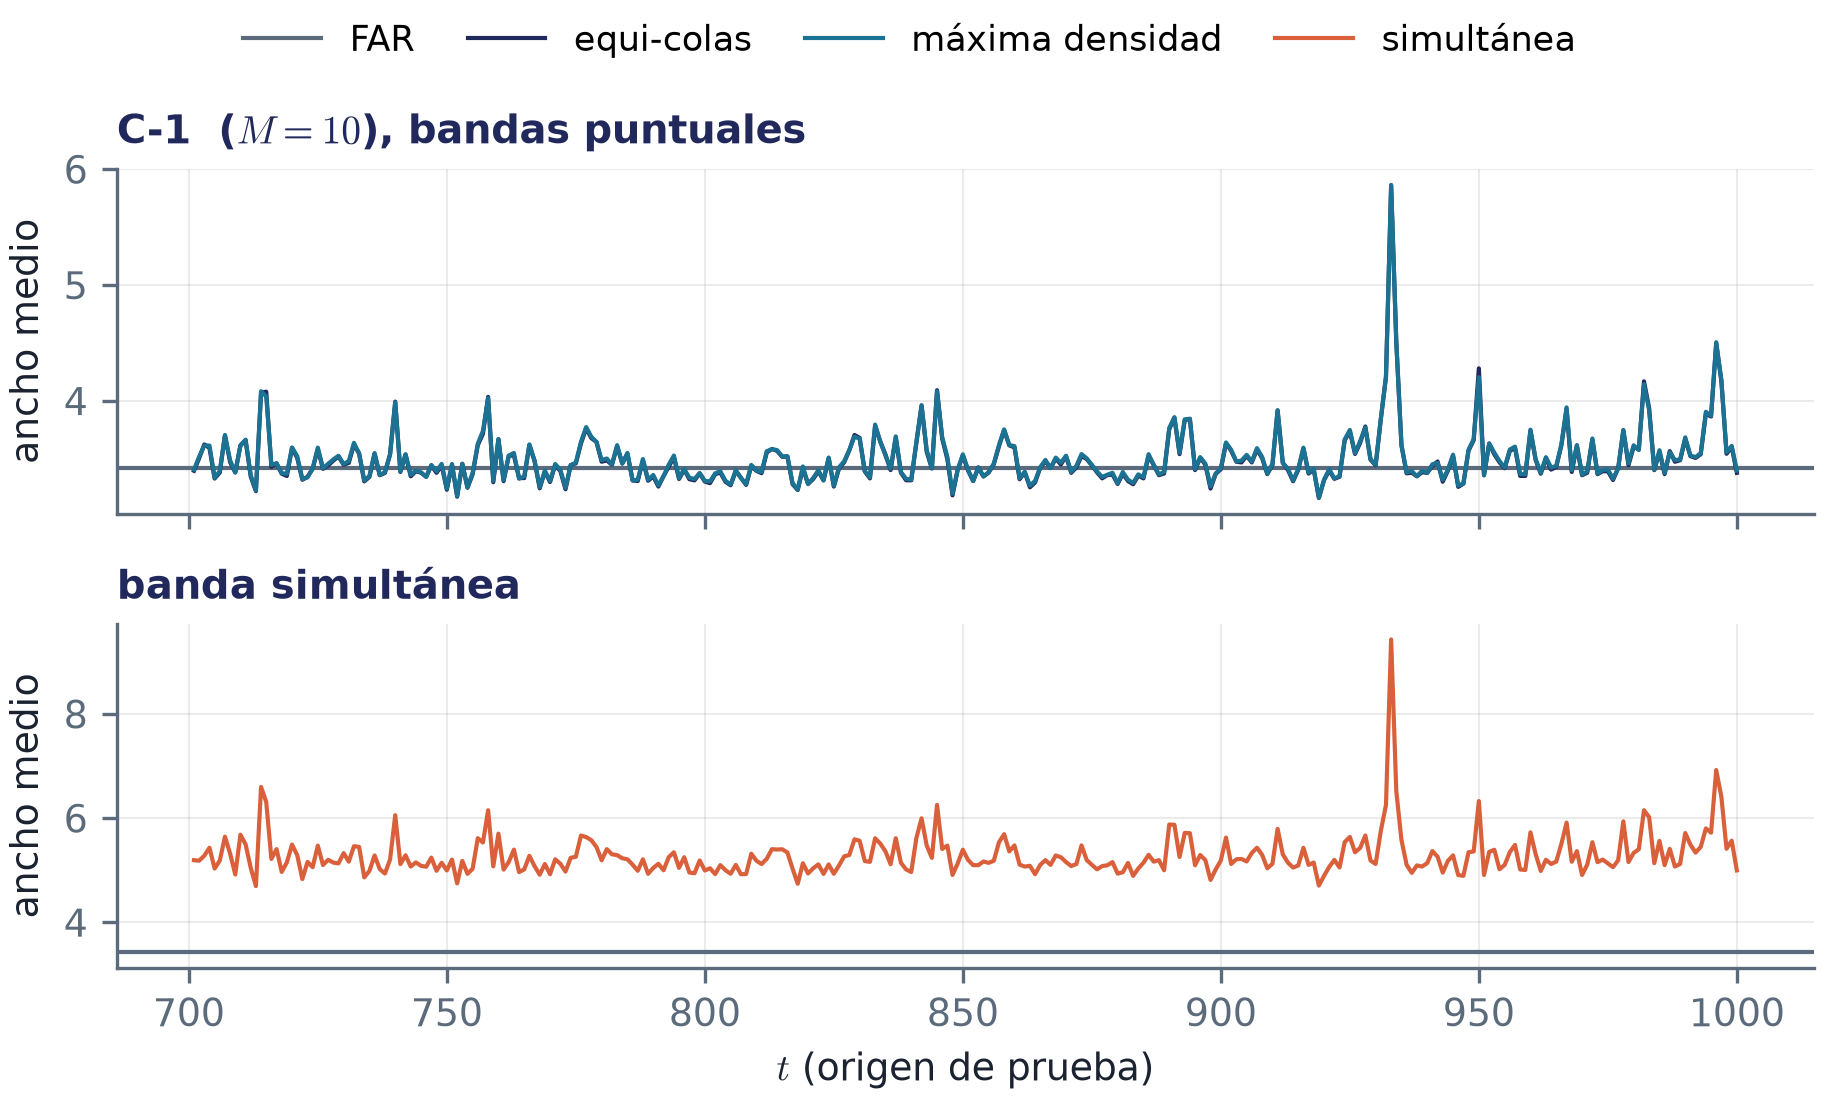
\includegraphics[width=\textwidth]{IMG/03_08/03_08_bloqueB_ancho_C1.png}
\caption{C-1. Ancho medio de la banda en cada origen de prueba ($M_{\mathrm{ref}}$) de las tres construcciones del PSBPM-FD y ancho fijo del FAR.}
\label{fig:res_bloqueB_ancho_C1}
\end{figure}

\begin{figure}[H]
\centering
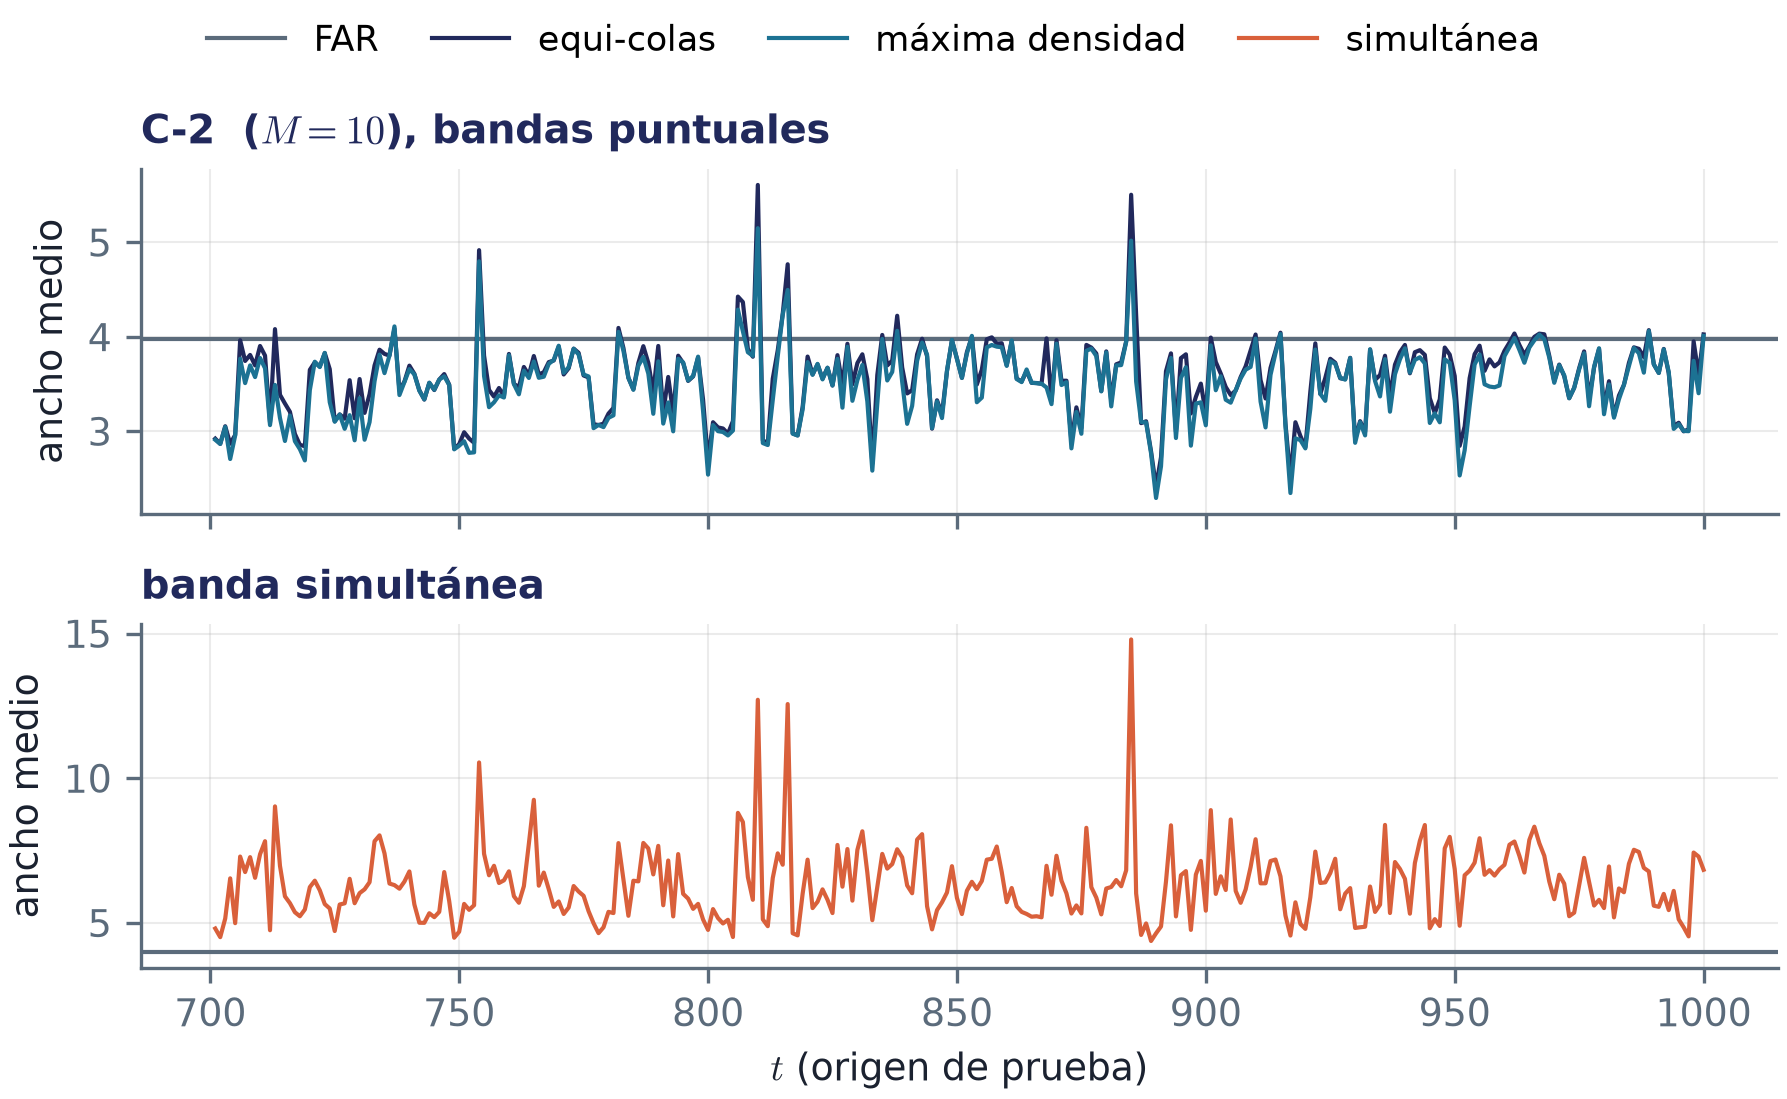
\includegraphics[width=\textwidth]{IMG/03_08/03_08_bloqueB_ancho_C2.png}
\caption{C-2. Ancho medio de la banda en cada origen de prueba ($M_{\mathrm{ref}}$) de las tres construcciones del PSBPM-FD y ancho fijo del FAR.}
\label{fig:res_bloqueB_ancho_C2}
\end{figure}

\begin{figure}[H]
\centering
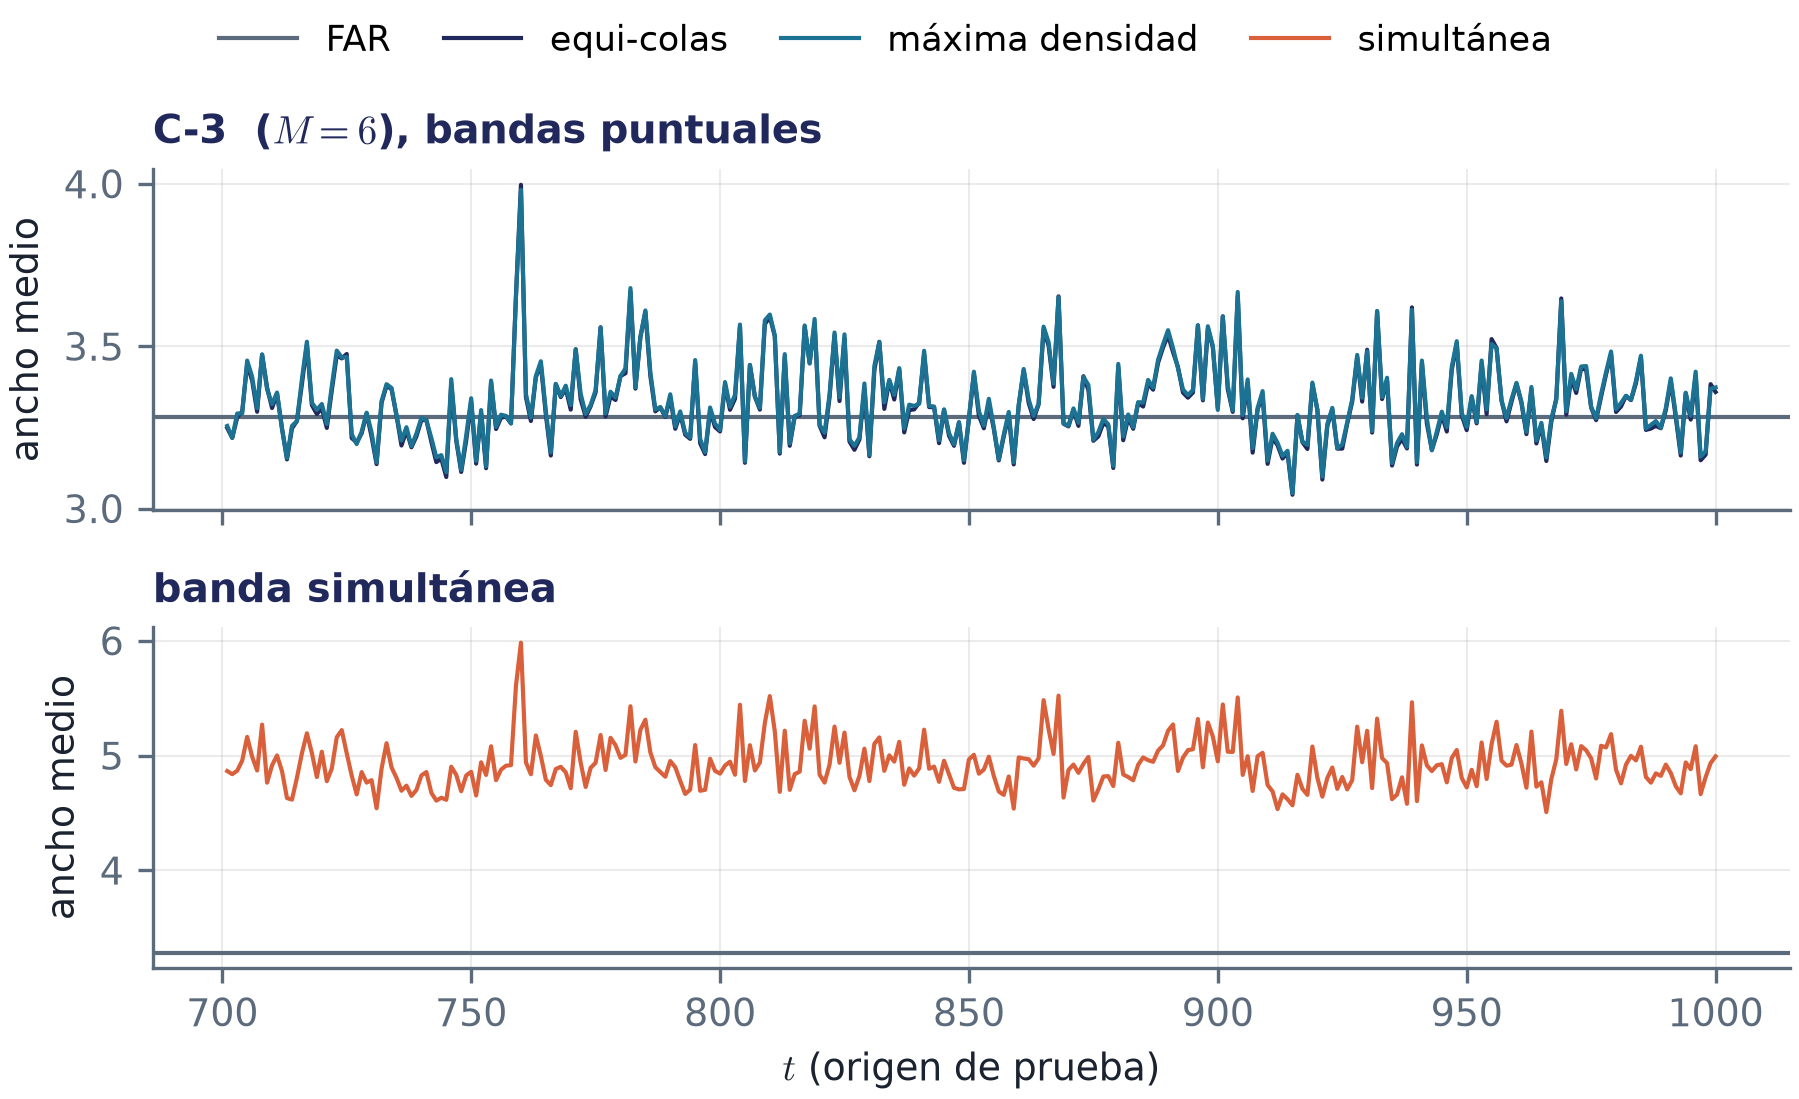
\includegraphics[width=\textwidth]{IMG/03_08/03_08_bloqueB_ancho_C3.png}
\caption{C-3. Ancho medio de la banda en cada origen de prueba ($M_{\mathrm{ref}}$) de las tres construcciones del PSBPM-FD y ancho fijo del FAR.}
\label{fig:res_bloqueB_ancho_C3}
\end{figure}

\subsection{Comportamientos predictivos}
\label{03_08_03_comportamientos}

Esta subsección y la siguiente se restringen a C-2. En C-1 y C-3 el modelo declara un solo comportamiento en el $99.7\%$ y el $100\%$ de los orígenes de prueba, como anticipa el diseño de la Sección~\ref{03_07_00_diseno_estudio_simulacion}. En C-2 se reporta primero cuántos comportamientos declara el modelo en el bloque de prueba completo para cada $M$ del barrido (Cuadro~\ref{tab:res_K}) y cómo se compara con los que tiene la ley verdadera. Luego se examinan de cerca diez orígenes consecutivos para mostrar qué es un comportamiento y qué ofrece frente a la esperanza (Figura~\ref{fig:res_ventana_detalle_C2}).

% Fuente: 102_K_por_M.csv de la 300 (bloque test).
\begin{table}[H]
\centering\small
\caption{Distribución de $K_t$ en el bloque de prueba de C-2 por $M$.}
\label{tab:res_K}
\begin{tabular}{c ccc}
\hline
$M$ & $K_t = 1$ & $K_t = 2$ & $K_t \ge 3$ \\
\hline
$1$ & 68.7\% & 31.3\% & 0.0\% \\
$2$ & 70.0\% & 15.7\% & 14.3\% \\
$3$ & 69.7\% & 15.7\% & 14.7\% \\
$4$ & 69.3\% & 16.7\% & 14.0\% \\
$5$ & 69.7\% & 16.7\% & 13.7\% \\
$6$ & 70.3\% & 16.3\% & 13.3\% \\
$7$ & 69.7\% & 16.7\% & 13.7\% \\
$8$ & 69.7\% & 16.7\% & 13.7\% \\
$9$ & 70.0\% & 16.7\% & 13.3\% \\
$10$ & 70.0\% & 16.7\% & 13.3\% \\
\hline
\end{tabular}
\end{table}

% Lectura K: los comportamientos aparecen donde la ley condicional reparte masa entre átomos separados.
En C-2 los comportamientos los producen los scores que cambian de régimen, ya que cerca del umbral los dos regímenes de un score son posibles a la vez y la mezcla pone un átomo en cada uno, de modo que el número de comportamientos lo fijan los scores con cambio de régimen y no cuántos scores entran al modelo. El Cuadro~\ref{tab:res_K} lo muestra en el barrido. Con $M = 1$ hay a lo más dos comportamientos, los dos regímenes del primer score. Con $M = 2$ aparece el tercero, porque el segundo score puede estar en un régimen distinto del primero y la mezcla separa esa combinación. Desde ahí la distribución no cambia con $M$, y los seis scores pasivos son autorregresivos sin regímenes, así que no abren comportamientos nuevos por más que se agreguen. Es lo que corresponde a la simulación, en que la dinámica de régimen vive en los primeros scores y el resto solo agrega variabilidad.\\

La ley verdadera tiene más de un modo en cerca de un $9\%$ de los orígenes de prueba, de modo que el modelo declara tres veces más de los que hay. La razón es que los pesos de la mezcla dependen de los rezagos a través de una transformación probit suave, que deja algo de masa en el átomo del régimen volátil también lejos del umbral, donde la probabilidad verdadera de ese régimen es casi nula. En los dos orígenes de la ventana de detalle en que la ley es bimodal, el modelo declara más de un comportamiento.\\

Las cifras anteriores resumen el bloque de prueba completo, pero no muestran qué es un comportamiento. Para eso se examinan de cerca $N_{\mathrm{det}} = 10$ orígenes consecutivos ($t = 807, \dots, 816$), el tramo del bloque de prueba con más cambios de régimen verdadero. 
% Figura: tres orígenes de la ventana de detalle de C-2. Fuente: comportamientos_psbp.npz y banda_funcional_psbp.npz del _04
% (curvas típicas, bandas condicionales, esperanza) y las curvas del generador.
\begin{figure}[H]
\centering
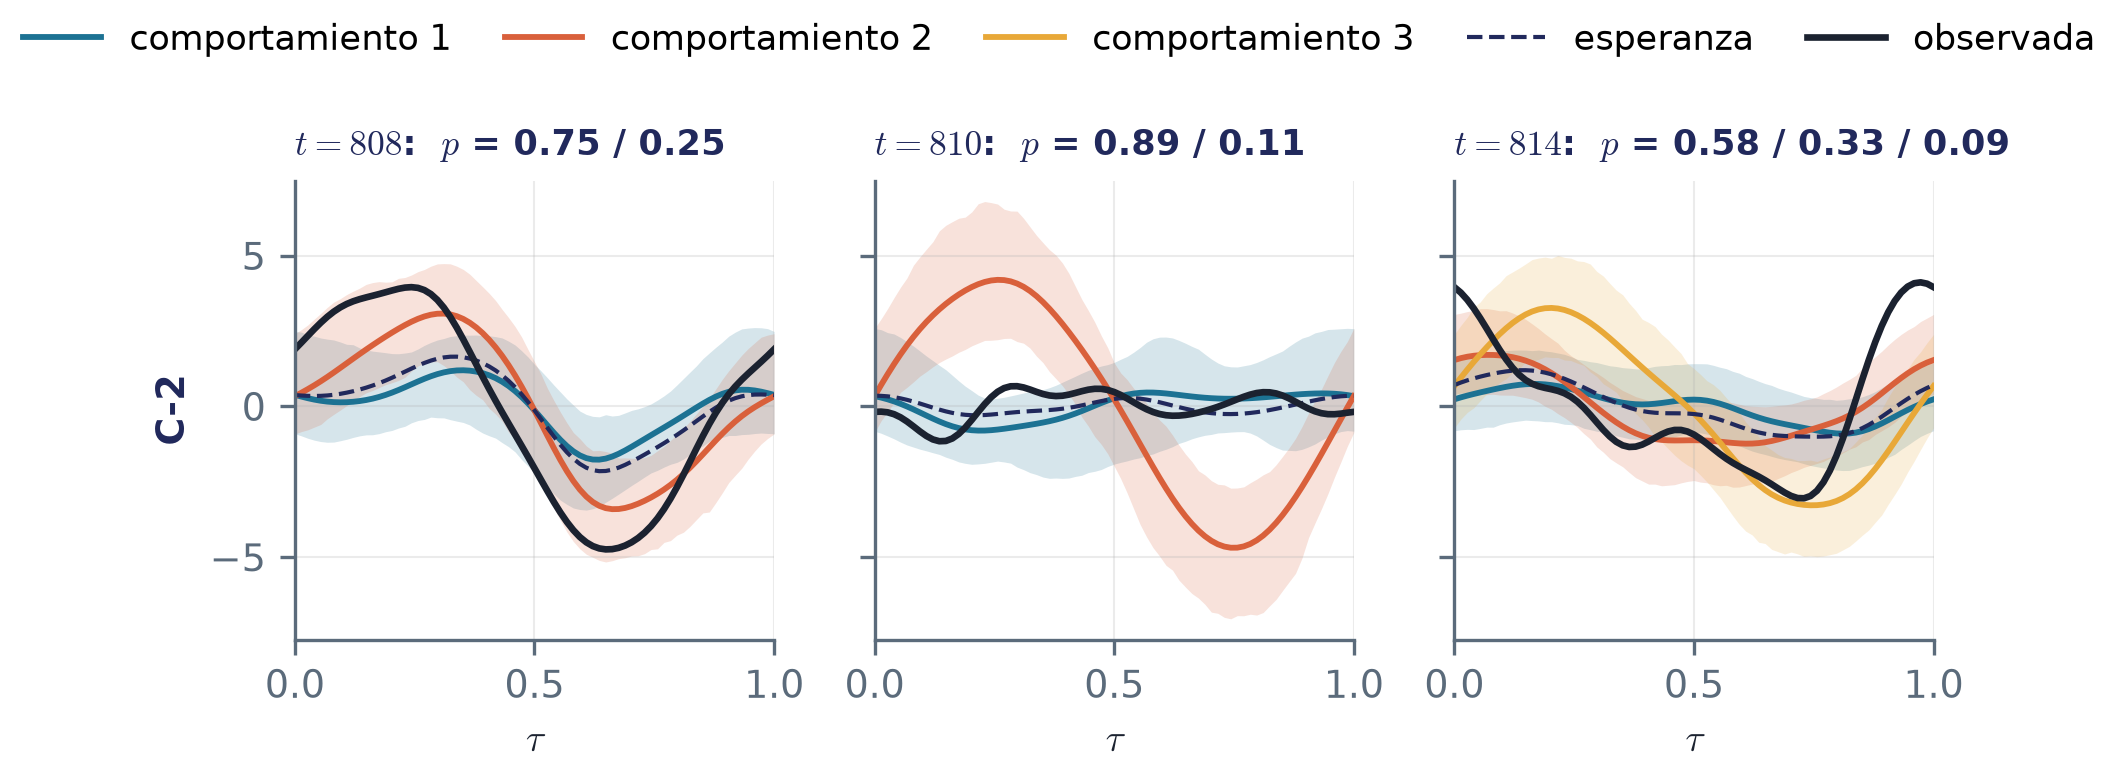
\includegraphics[width=\textwidth]{IMG/03_08/03_08_ventana_detalle_C2.png}
\caption{C-2. Tres orígenes de la ventana de detalle ($M_{\mathrm{ref}}$), con dos y tres comportamientos. Curva observada, esperanza y, por comportamiento, curva típica, banda condicional y probabilidad.}
\label{fig:res_ventana_detalle_C2}
\end{figure}

% Lectura detalle: para qué sirven los comportamientos y por qué el modelo acierta o falla en cada origen.
En los orígenes $807$ a $816$ el modelo declara más de un comportamiento en seis y la ley verdadera tiene más de un modo en dos, por la masa que los pesos probit dejan lejos del umbral, y aun así la curva observada cae en el comportamiento más probable en siete de los diez. En $t = 808$ el régimen cambió sin que el rezago lo anunciara y la curva observada sigue al comportamiento minoritario, cuya banda la cubre entera, mientras que la esperanza, que promedia los dos, queda en una curva que no ocurre. Es el caso en que una predictiva multimodal ofrece una opción que el promedio no tiene. En $t = 810$ acierta el más probable y el segundo es la masa que los pesos dejan en el régimen volátil. En $t = 814$ tres de los cuatro scores activos están en el régimen volátil, hay tres comportamientos y la curva observada se parece al segundo, pero sale de las bandas puntuales al final del dominio y solo la simultánea la contiene. Con qué frecuencia el comportamiento realizado es el más probable, y cuánto cuesta elegir mal, es lo que cuantifica la Sección~\ref{03_08_04_pronostico} sobre todo el bloque de prueba.

\subsection{Predicción por comportamiento}
\label{03_08_04_pronostico}

El Cuadro~\ref{tab:res_pronostico} resume, en $M_{\mathrm{ref}}$ de C-2, el error del pronóstico por comportamiento y de su cota \eqref{eq:mejor_comportamiento} frente a la esperanza y a las referencias, sobre todos los orígenes de prueba y sobre los que tienen más de un comportamiento. El Cuadro~\ref{tab:res_pronostico_por_M} y las Figuras~\ref{fig:res_pronostico_ventana_C2} y~\ref{fig:res_pronostico_ventana_rmse_C2} muestran lo mismo contra $M$ y sobre la ventana móvil, y el Cuadro~\ref{tab:res_acierto_p1} cuándo la elección por probabilidad acierta. Los dos cuadros promedian sobre los orígenes de prueba y no sobre las ventanas, porque el subconjunto con más de un comportamiento no es contiguo, y por eso sus cifras difieren en la tercera decimal de las de la Sección~\ref{03_08_01_error_puntual}.

% Fuente: 113_opciones_por_origen.csv del _06 (m10, test, opción "tipica"); MAE = media por origen, RMSE = raíz de la media de los cuadrados por origen. Coincide con 119_resumen_opciones_por_M.csv.
\begin{table}[H]
\centering\footnotesize
\caption{Pronóstico por comportamiento en el bloque de prueba de C-2 ($M_{\mathrm{ref}}$), sobre todos los orígenes y sobre los que tienen más de un comportamiento.}
\label{tab:res_pronostico}
\begin{tabular}{l cc cc}
\hline
 & \multicolumn{2}{c}{Todos los orígenes ($n = 300$)} & \multicolumn{2}{c}{$K_t \ge 2$ ($n = 90$)} \\
 & MAE & RMSE & MAE & RMSE \\
\hline
Pronóstico por comportamiento  & 0.607 & 0.793 & 0.619 & 0.847 \\
Cota (mejor comportamiento)    & 0.565 & 0.727 & 0.478 & 0.618 \\
Esperanza                      & 0.602 & 0.771 & 0.602 & 0.776 \\
FAR                            & 0.769 & 0.981 & 0.748 & 0.971 \\
Random Forest                  & 0.584 & 0.760 & 0.559 & 0.737 \\
\hline
\multicolumn{5}{l}{Fracción de orígenes} \\
El pronóstico gana al FAR            & \multicolumn{2}{c}{84\%} & \multicolumn{2}{c}{83\%} \\
El pronóstico gana al Random Forest  & \multicolumn{2}{c}{44\%} & \multicolumn{2}{c}{44\%} \\
La cota gana al FAR                  & \multicolumn{2}{c}{88\%} & \multicolumn{2}{c}{96\%} \\
La cota gana al Random Forest        & \multicolumn{2}{c}{49\%} & \multicolumn{2}{c}{61\%} \\
\hline
\end{tabular}
\end{table}

% Lectura pronóstico: elegir es una apuesta. Gana al FAR, no a la esperanza en promedio, y la cota dice cuánto hay en juego.
Elegir el comportamiento más probable es una apuesta, y por tanto, sobre todos los orígenes el pronóstico empata con la esperanza en MAE (0.607 frente a 0.602), porque en siete de cada diez coincide con ella, y es algo peor en RMSE. Las diferencias aparecen en los orígenes con más de un comportamiento, que muestra el Cuadro~\ref{tab:res_pronostico}. Frente al FAR gana con holgura, en el 83\% de ellos, porque cualquiera de los comportamientos es la curva de un régimen y el operador lineal no puede dar ninguna de ellas. Frente a la esperanza gana en el 59\% de esos orígenes y aun así pierde en promedio, porque cuando acierta el error baja, pero cuando el elegido no es el mejor el error sube más de lo que se ganó, porque la curva típica elegida queda lejos de la observada, mientras que la esperanza, al promediar, nunca queda tan lejos. Es el mismo motivo por el que el RMSE prefiere la esperanza. La cota dice cuánto hay en juego. En los orígenes con más de un comportamiento baja el error un quinto respecto de la esperanza y queda bajo el Random Forest, que es el mejor predictor puntual de C-2, de modo que entre las opciones que entrega el modelo casi siempre está la buena y lo que se pierde es por elegirla con la probabilidad, que acierta en el 78\% de esos orígenes. Sobre todos los orígenes, donde en siete de cada diez no hay nada que elegir, la ventaja de la cota es de un 6\% sobre la esperanza.

% Fuente: 113_opciones_por_origen.csv de cada M del _06 (test, opción "tipica"), medias por origen como en tab:res_pronostico.
\begin{table}[H]
\centering\footnotesize
\setlength{\tabcolsep}{3pt}
\caption{MAE y RMSE en el bloque de prueba de C-2 por $M$ del pronóstico por comportamiento, de la cota, de la esperanza, del FAR y del Random Forest.}
\label{tab:res_pronostico_por_M}
\begin{tabular}{c ccccc ccccc}
\hline
 & \multicolumn{5}{c}{MAE} & \multicolumn{5}{c}{RMSE} \\
$M$ & Pronóstico & Cota & Esperanza & FAR & RF & Pronóstico & Cota & Esperanza & FAR & RF \\
\hline
$1$ & 0.711 & 0.693 & 0.711 & 0.769 & 0.707 & 0.912 & 0.882 & 0.905 & 0.981 & 0.904 \\
$2$ & 0.670 & 0.636 & 0.666 & 0.769 & 0.651 & 0.862 & 0.811 & 0.849 & 0.981 & 0.838 \\
$3$ & 0.632 & 0.596 & 0.628 & 0.769 & 0.610 & 0.816 & 0.763 & 0.802 & 0.981 & 0.789 \\
$4$ & 0.612 & 0.570 & 0.605 & 0.769 & 0.584 & 0.799 & 0.733 & 0.777 & 0.981 & 0.762 \\
$5$ & 0.610 & 0.567 & 0.604 & 0.769 & 0.584 & 0.797 & 0.730 & 0.775 & 0.981 & 0.761 \\
$6$ & 0.608 & 0.568 & 0.603 & 0.769 & 0.585 & 0.795 & 0.730 & 0.773 & 0.981 & 0.761 \\
$7$ & 0.608 & 0.566 & 0.603 & 0.769 & 0.584 & 0.794 & 0.728 & 0.772 & 0.981 & 0.761 \\
$8$ & 0.608 & 0.565 & 0.603 & 0.769 & 0.584 & 0.793 & 0.727 & 0.772 & 0.981 & 0.761 \\
$9$ & 0.608 & 0.565 & 0.602 & 0.769 & 0.584 & 0.793 & 0.727 & 0.772 & 0.981 & 0.761 \\
$10$ & 0.607 & 0.565 & 0.602 & 0.769 & 0.584 & 0.793 & 0.727 & 0.771 & 0.981 & 0.760 \\
\hline
\end{tabular}
\end{table}

% Lectura trayectoria: la brecha entre cota y pronóstico está repartida en todo el test (contra M, 113 de cada M, no se tabula).
El Cuadro~\ref{tab:res_pronostico_por_M} muestra que la brecha entre la cota y el pronóstico se abre ya con $M = 1$ y deja de crecer en $M = 4$, como el resto del error puntual, porque los comportamientos los fijan los primeros scores. Las Figuras~\ref{fig:res_pronostico_ventana_C2} y~\ref{fig:res_pronostico_ventana_rmse_C2} muestran que la cota queda bajo la esperanza en todas las ventanas del bloque de prueba y bajo el pronóstico en el 87\% de ellas, porque los orígenes con más de un comportamiento están repartidos en él. La separación es mayor en el tramo de más cambios de régimen, donde el pronóstico queda por encima de la esperanza en todas las ventanas, porque ahí es donde más veces se elige mal.

% Figura: pronóstico y cota sobre la ventana móvil de prueba, w_ref, M_ref, contra FAR, RF y esperanza. Fuente: 115_ventana_modelos_w30.csv del _06.
\begin{figure}[H]
\centering
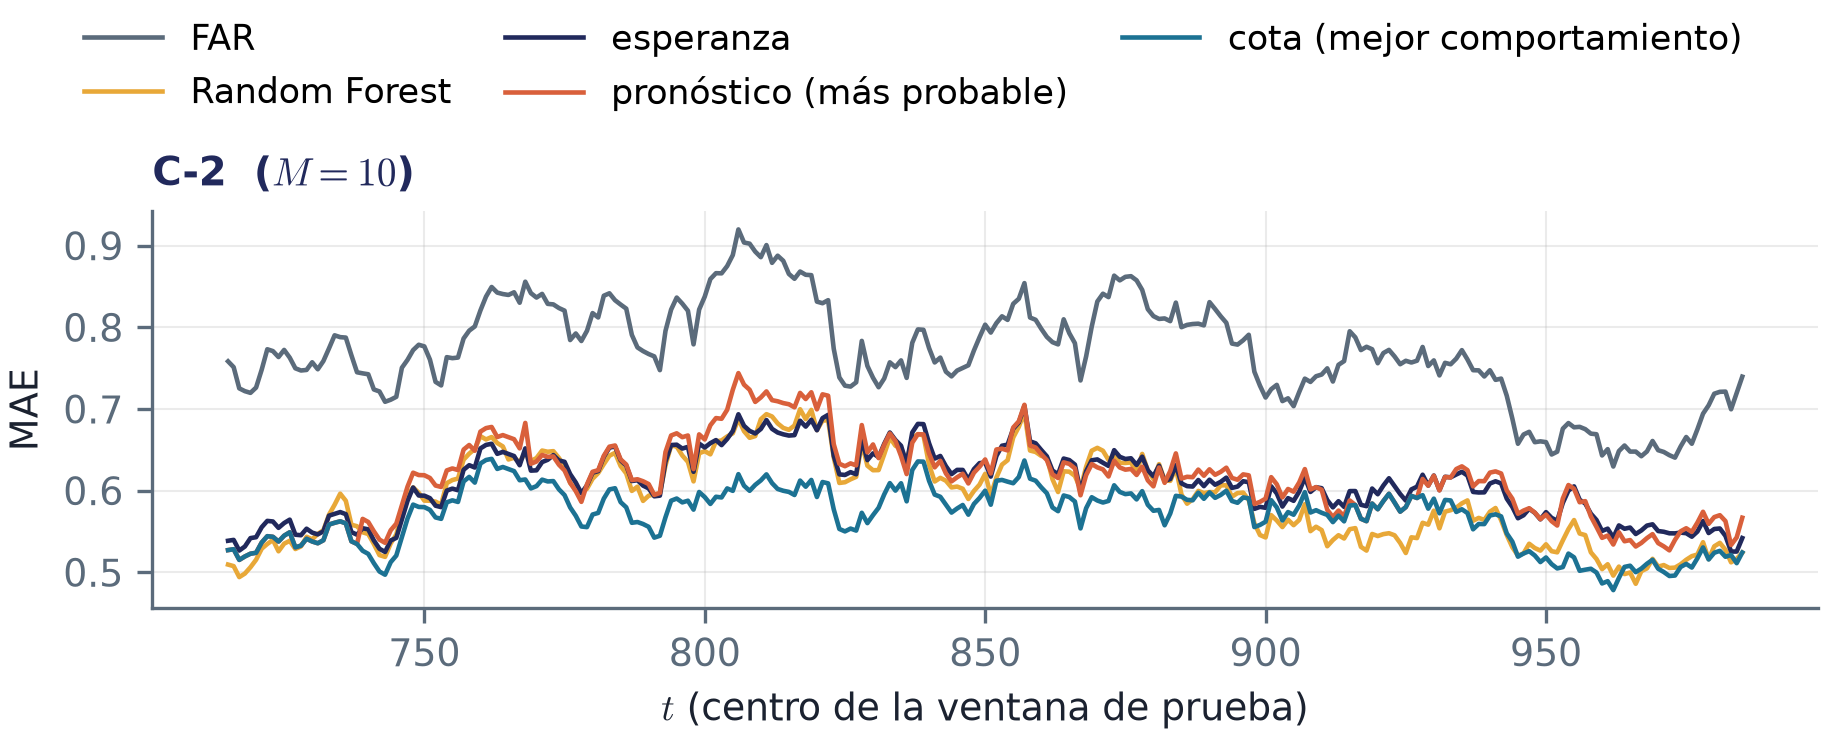
\includegraphics[width=\textwidth]{IMG/03_08/03_08_pronostico_ventana_w30_C2.png}
\caption{C-2. MAE del pronóstico por comportamiento y de la cota sobre la ventana móvil del bloque de prueba ($M_{\mathrm{ref}}$).}
\label{fig:res_pronostico_ventana_C2}
\end{figure}

\begin{figure}[H]
\centering
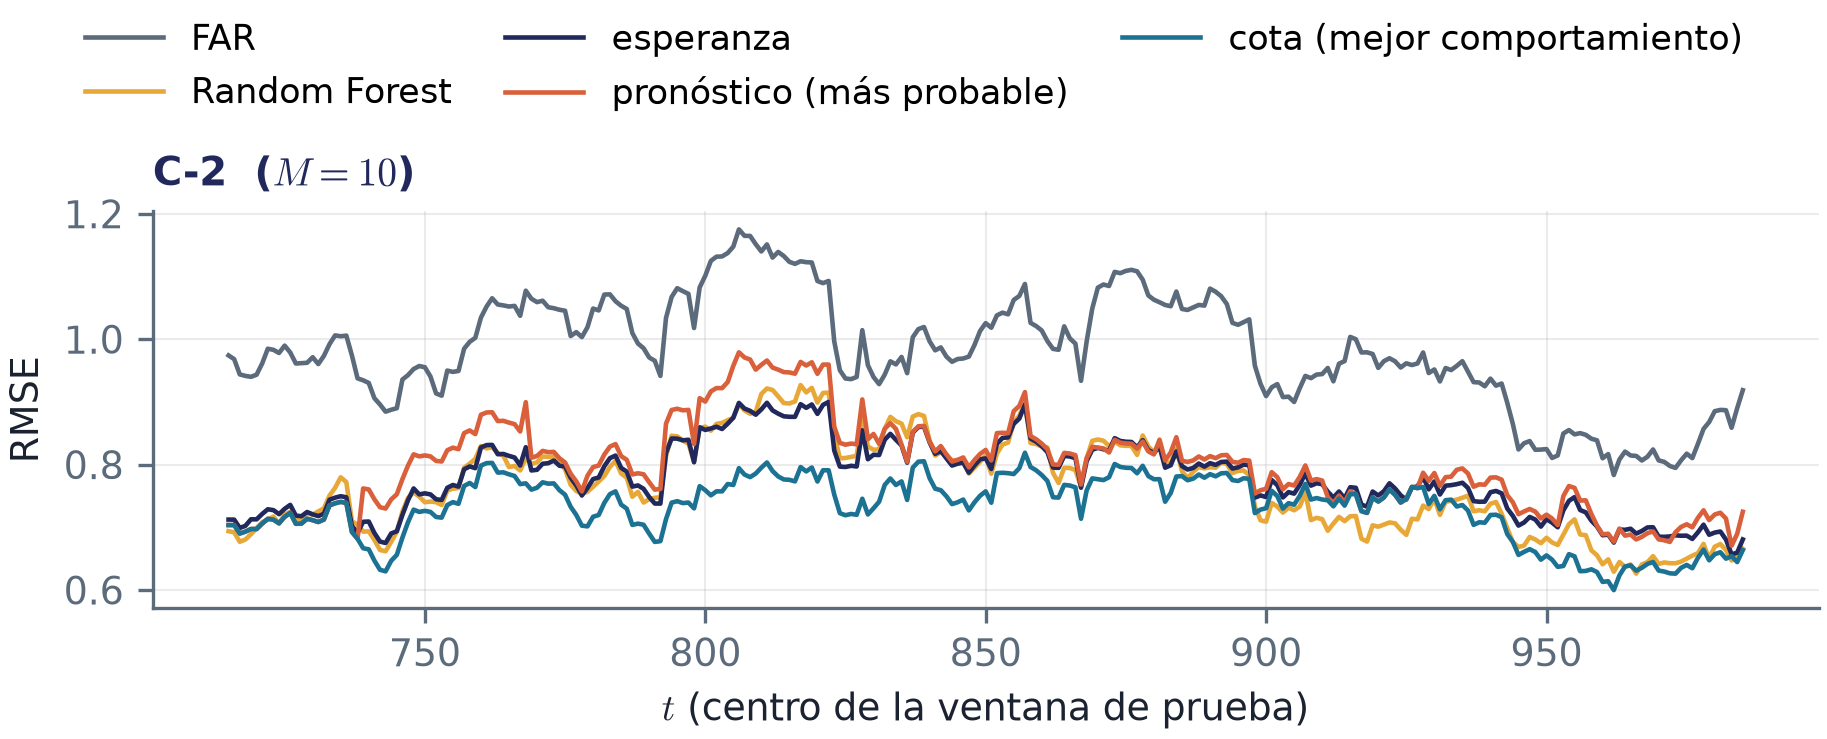
\includegraphics[width=\textwidth]{IMG/03_08/03_08_pronostico_ventana_rmse_w30_C2.png}
\caption{C-2. RMSE del pronóstico por comportamiento y de la cota sobre la ventana móvil del bloque de prueba ($M_{\mathrm{ref}}$).}
\label{fig:res_pronostico_ventana_rmse_C2}
\end{figure}

% Fuente: 119_acierto_por_p1.csv del _06 (test, K >= 2, M_ref). 83 de los 90 orígenes tienen p >= 0.5; los 7 restantes tienen K = 3 sin comportamiento dominante.
\begin{table}[H]
\centering\small
\caption{Acierto del pronóstico por comportamiento en C-2 ($K_t \ge 2$, $M_{\mathrm{ref}}$) por tramo de la probabilidad del comportamiento elegido. La última columna es el MAE que se pierde por elegir con la probabilidad en vez de la cota, en promedio sobre los orígenes del tramo. Los siete orígenes sin comportamiento dominante no se tabulan.}
\label{tab:res_acierto_p1}
\begin{tabular}{l c c c}
\hline
$p_{t,k^{*}}$ & Orígenes & Acierto & MAE pronóstico $-$ MAE cota \\
\hline
$[0.5, 0.6)$ & 5  & 20\%  & 0.61 \\
$[0.6, 0.7)$ & 11 & 36\%  & 0.28 \\
$[0.7, 0.8)$ & 31 & 87\%  & 0.11 \\
$[0.8, 0.9)$ & 28 & 93\%  & 0.06 \\
$[0.9, 1]$   & 8  & 100\% & 0.00 \\
\hline
\end{tabular}
\end{table}

% Lectura acierto: la probabilidad dice cuándo apostar. Entre 0.5 y 0.7 el acierto queda bajo una moneda y concentra cerca de la mitad de la pérdida.
La probabilidad del comportamiento elegido dice cuándo conviene apostar, como muestra el Cuadro~\ref{tab:res_acierto_p1}. Con una probabilidad alta el elegido es el mejor casi siempre y el pronóstico queda a un paso de la cota. Con masas entre un medio y $0.7$ el acierto cae por debajo de lo que daría una moneda, 5 de 16 orígenes en conjunto, y ahí se concentra cerca de la mitad de la pérdida. Con tan pocos orígenes no se puede separar si se debe al origen, con rezagos sobre el umbral donde el propio generador sortea el régimen con probabilidad cercana a un medio, o a una probabilidad optimista del modelo, coherente con la sobredetección de comportamientos de la Sección~\ref{03_08_03_comportamientos}. Tres de cada cuatro orígenes con más de un comportamiento tienen $p_{t,k^{*}} \ge 0.7$, y ahí el pronóstico queda cerca de la cota. Con una probabilidad alta se pronostica con el comportamiento, con una baja se reportan las opciones.

\section{Discusión}
\label{03_09}

En la predicción puntual, el PSBPM-FD supera al FAR en los tres escenarios, y lo hace de forma sostenida a lo largo del bloque de prueba y no solo en promedio. En C-2, donde la media condicional es no lineal, la esperanza reduce el MAE y el RMSE en torno a un $21\%$ y supera al FAR en todas las ventanas de prueba. En C-1 y C-3, donde la media condicional es lineal o casi lineal y la referencia está casi bien especificada, la reducción promedio es cercana al $2\%$, pero se repite en cerca de nueve de cada diez ventanas, y alguno de los tres predictores del PSBPM-FD es el mejor modelo en el $82\%$ y el $74\%$ de ellas. Una diferencia pequeña en el promedio corresponde, por tanto, a una ventaja consistente y no a unos pocos tramos favorables. Entre los predictores, la esperanza es la mejor bajo RMSE y la mediana puntual bajo MAE donde la predictiva es multimodal, como corresponde a la pérdida que cada una minimiza, y el átomo más probable es el más débil. En C-1 y C-2 el error deja de bajar en $M = 4$, la dimensión en que se observa toda la dinámica del generador; en C-3, donde los rezagos de todas las componentes entran a los pesos, el mínimo está en $M = 5$.\\

El Random Forest, con las mismas covariables, tiene un error mayor que el FAR en C-1 y queda por detrás del PSBPM-FD en más del $80\%$ de las ventanas de C-1 y C-3, pero es el mejor predictor puntual de C-2, en promedio y en dos de cada tres ventanas. Esto es coherente con la estructura de umbral del escenario, que sus cortes reproducen directamente, mientras que los pesos probit del PSBPM-FD cambian de forma suave. Aun así, la curva que lo supera suele estar entre las opciones de la predictiva del PSBPM-FD, ya que su cota tiene un MAE menor que el del Random Forest, sobre todo en los orígenes con más de un comportamiento ($0.478$ frente a $0.559$). La cota no es un predictor, de modo que la comparación no es justa en la práctica, pero indica que la desventaja del PSBPM-FD está en resumir una predictiva multimodal en una sola curva y no en la información que contiene.\\

Los intervalos son donde el modelo muestra su ventaja más clara. Las bandas puntuales del PSBPM-FD reducen el Winkler del FAR en un $20\%$ a $22\%$ en C-2 y en cerca de un $3\%$ en C-1 y C-3, y lo superan en entre el $73\%$ y el $100\%$ de las ventanas. En C-2 la reducción viene a la vez de una banda un $10\%$ más angosta y de una mayor cobertura; en C-1 y C-3, de una mejor calibración. La razón es que el ancho de la banda del PSBPM-FD se adapta al estado del proceso, angosta en los tramos tranquilos y ancha en los episodios de mayor varianza o en el régimen volátil, mientras que la banda del FAR hereda una varianza residual fija y tiene el mismo ancho en todos los orígenes. Esa adaptación es la que una ley de error rígida no puede dar, y es la razón por la que la ventaja en los intervalos aparece incluso donde la media condicional es lineal. La región de máxima densidad solo se separa de la equi-colas en C-2, donde la predictiva tiene valles, y ahí es la mejor banda en nueve de cada diez ventanas. La banda simultánea pierde el Winkler por ser más ancha, pero es la única que cubre la curva completa con una frecuencia cercana a la nominal.\\

Los comportamientos predictivos responden a los cambios de régimen. En C-2 la predictiva tiene más de un comportamiento en el $30\%$ de los orígenes de prueba, y su número lo fijan los scores con cambio de régimen y no la dimensión $M$. En C-1 y C-3 la predictiva tiene un solo comportamiento en casi todos los orígenes. En C-3 la multimodalidad del generador queda en la ley conjunta de los scores y no llega a la curva, de modo que los comportamientos detectan los modos de la curva siguiente y no los de cualquier mecanismo latente. El pronóstico con el comportamiento más probable empata con la esperanza en MAE sobre todo el bloque de prueba y la supera en el $59\%$ de los orígenes con más de un comportamiento, pero pierde en promedio porque las elecciones equivocadas pesan más que las acertadas. Su cota reduce el error de la esperanza en un quinto, de modo que la opción correcta suele estar entre las que entrega el modelo y la pérdida se produce al elegirla. La probabilidad del comportamiento elegido indica cuándo conviene hacerlo.\\

Los comportamientos admiten además una lectura como agrupamiento. Cuando el cambio de régimen lo gobierna una variable latente que los rezagos revelan solo en parte, los comportamientos funcionan como un agrupamiento de la curva siguiente por estado latente, con la probabilidad de cada uno. En C-2 el agrupamiento sigue al régimen del generador; el capítulo siguiente examina el caso de un estado latente en datos reales.\\

La principal limitación de los comportamientos es la sobredetección. El modelo declara más de un comportamiento en el $30\%$ de los orígenes de prueba de C-2, mientras que la ley verdadera es multimodal solo en cerca de un $9\%$, porque la transición probit suave deja masa en el régimen volátil lejos del umbral. En la misma línea, cuando la probabilidad del comportamiento elegido está entre $0.5$ y $0.7$, el acierto es de 5 en 16 orígenes, por debajo de lo que esa probabilidad indica; con tan pocos orígenes no puede separarse si se debe a rezagos sobre el umbral o a una probabilidad optimista del modelo.\\

En la práctica, el resumen que conviene reportar depende de la forma de la predictiva en cada origen, que los comportamientos permiten leer. Cuando la predictiva tiene un solo comportamiento, la esperanza resume bien la curva siguiente; cuando tiene más de uno, conviene acompañarla de la mediana puntual o del pronóstico por comportamiento, según la probabilidad de cada opción. Entre los intervalos, la banda equi-colas es la construcción de referencia, la simultánea es la opción conservadora cuando interesa cubrir la curva completa, a costa de un ancho mayor, y la de máxima densidad es la más ajustada cuando la predictiva tiene valles. En cuanto a la dimensión, con rezagos propios agregar componentes no empeora el error puntual, que se estabiliza una vez cubiertos los scores con dinámica, mientras que con los rezagos de todas las componentes cada score adicional agranda el conjunto de covariables de los pesos de la mezcla y uno sin dinámica puede empeorarlo, como ocurre en C-3 con $M = 6$. La factorización hace además que los $M$ muestreadores sean independientes y puedan ejecutarse en paralelo, y con rezagos propios basta entrenar el mayor $M$ del barrido y reutilizar sus trazas para los menores.










